% #132 | Archive/SP_SauLuoi_2024-2025/SP_HKI/2-TN-DS-TLN-SGD-BacGiang-HKI-NH24-25.tex | mã gốc 2D4V3-2
\begin{ex}%[2D4V3-2]%[Dự Án Đợt 4 - De Thi HK1-2024-2025]%[Thầy Hải Toán]
\immini
{
Một vật chuyển động trong $4$ giờ với vận tốc $v$ (km/h) phụ thuộc thời gian $t$ (h) có đồ thị của vận tốc như hình bên. Trong khoảng thời gian $2$ giờ kể từ khi bắt đầu chuyển động, đồ thị đó là một phần của đường Parabol có đỉnh $I(2;7)$ và trục đối xứng của Parabol song song với trục tung, khoảng thời gian còn lại đồ thị là đoạn thẳng $IA$. Tìm độ dài quãng đường mà vật di chuyển được trong $4$ giờ đó (làm tròn kết quả đến hàng phần mười)	
}
{
\begin{tikzpicture}[line join = round, line cap = round,>=stealth,font=\footnotesize,scale=0.7]
	\def\xmin{-1} \def\xmax{5}
	\def\ymin{-1} \def\ymax{8} 
	\foreach \x in {2,4} \draw (\x,2pt)--(\x,-2pt) node [below] {$\x$};
	\draw[-stealth] (\xmin,0)--(\xmax,0)node[below]{$t$}; 
	\foreach \y in {3,7} \draw (2pt,\y)--(-2pt,\y) node [left] {$\y$}; 
	\draw[-stealth] (0,\ymin)--(0,\ymax)node[right]{$v$};
	\foreach \x/\y in {0/3,0/7,2/7,4/3} \fill (\x,\y) circle (1.5pt);
	\filldraw (0,0)node[below left]{$O$} circle (1.5pt); 
	\clip (\xmin,\ymin) rectangle (\xmax,\ymax);  
	\draw[samples=100,domain=0:2,smooth,red] plot (\x,{-(\x)^2+4*(\x)+3});
	\draw[samples=100,domain=2:4,smooth,red,dashed] plot (\x,{-(\x)^2+4*(\x)+3});
	\draw (2,7)node[above]{$I$}--(4,3)node[right]{$A$};
	\draw[dashed] (0,3)-|(4,0) (0,7)-|(2,0);
\end{tikzpicture}	
}	
\shortans[oly]{$21{,}3$}
\loigiai{
Gọi $y=ax^2+bx+c$ là phương trình của đường Parabol đi qua điểm $(0;3)$ và có đỉnh là $I(2;7)$.\\
Parabol đi qua $(0;3)\Rightarrow c=3$.\\
Đỉnh $I(2;7)\Rightarrow 4a+2b+3=7\Rightarrow 2a+b=2$.\\
Trục đối xứng $x=-\dfrac{b}{2a}=2\Rightarrow 4a+b=0$.\\
Vậy ta có hệ phương trình $\heva{& 2a+b=2 \\ & 4a+b=0}\Rightarrow\heva{& a=-1 \\ & b=4.}$\\
Vậy phương trình đường Parabol là $y=-x^2+4x+3$.\\
Đường thẳng $IA$ có phương trình $y=ax+b$ đi qua $(2;7)$ và $(4;3)$ nên ta có hệ phương trình $\heva{& 2a+b=7 \\ & 4a+b=3}\Leftrightarrow\heva{& a=-2 \\ & b=11}\Rightarrow IA\colon y=-2x+11$.\\
Quãng đường vật chuyển động được là \[S=\displaystyle\int\limits_{0}^{2} \left(-x^2+4x+3\right) \mathrm{\,d}x +\displaystyle\int\limits_{2}^{4} \left(-2x+11\right) \mathrm{\,d}x=\dfrac{64}{3}\approx 21{,}3.\]
}
\end{ex}

% #351 | Archive/SP_SauLuoi_2024-2025/Sp_GHKII/data/GHKII/2-TL-TN-DS-THPT-NguyenThaiBinh-TpHCM-GHKII-NH24-25.tex | mã gốc 2D4H2-6
\begin{ex}%[2D4H2-6]%[Dự án đề kiểm tra Toán GHKII NH24-25- Phan Anh]%[THPT Nguyễn Thái Bình - Tp HCM]
Một vật chuyển động với tốc độ $v(t)=3t+4$\,(m/s), với thời gian $t$ tính theo giây, $t\in[0;5]$. Tính quãng đường (đơn vị: mét) vật đi được trong khoảng thời gian từ $t=0$ đến $t=5$.
\par\shortans[oly]{57,5}
\loigiai{Quãng đường (đơn vị: mét) vật đi được trong khoảng thời gian từ $t=0$ đến $t=5$ là
\[S=\displaystyle\int\limits_0^5v(t)\mathrm{\,d}t=\displaystyle\int\limits_0^5(3t+4)\mathrm{\,d}t=\dfrac{115}{2}=57{,}5\text{\,m.}\]}
\end{ex}

% #356 | Archive/SP_SauLuoi_2024-2025/Sp_GHKII/data/GHKII/2-TN-DS-TLN-thpt-thuan-thanh-1-2-3-bac-ninh-GHKII-NH24-25.tex | mã gốc 2D4H3-5
\begin{ex}%[2D4H3-5][Dự án đề kiểm tra Toán 12 GHKII NH24-25- Lê Hồ Quang Minh]%[THPT Thuận Thành 1-2-3 - Bắc Ninh]
	Một vật chuyển động đều với vận tốc có phương trình $v(t)=t^2-2 t+1$, trong đó $t$ được tính bằng giây, quãng đường $s(t)$ được tính bằng mét.
	\choiceTF
	{\True Quãng đường vật đi được từ khi vật bắt đầu chuyển động đến khi gia tốc bị triệt tiêu là $\dfrac{1}{3}$ m}
	{Quãng đường vật đi được trong 2 giây tính đến thời điểm mà vận tốc đạt $9(\mathrm{m} / \mathrm{s})$ là $\dfrac{26}{3}$ m}
	{\True Quãng đường đi được của vật sau 2 giây kể từ khi vật bắt đầu chuyển động là $\dfrac{2}{3}$ m}
	{Quãng đường vật đi được từ 0 giây đến thời điểm mà gia tốc bằng $10(\mathrm{m} / \mathrm{s}^2)$ là $44$ m}
	\loigiai{
		\begin{itemchoice}
			\itemch Gia tốc tức thời của vật là $a(t)=v'(t)=2t-2$.\\
			Gia tốc triệt tiêu khi $a(t)=0 \Leftrightarrow t=1$. Tức là gia tốc triệt tiêu tại thời điểm $t=1$ giây.\\
			Vậy quãng đường vật đi được từ khi bắt đầu chuyển động đến khi gia tốc triệt tiêu là\\
			\begin{center}
				$s=\displaystyle \int \limits_0^{1} (t^2-2t+1) \mathrm{~d}t=\dfrac{1}{3}$ m.
			\end{center}
			\itemch Cho $v(t)=9 \Leftrightarrow t=4$.\\
			Quãng đường vật đi được trong 2 giây tính đến thời điểm mà vận tốc đạt $9(\mathrm{m} / \mathrm{s})$ là\\
			\begin{center}
				$s=\displaystyle \int \limits_4^{6} (t^2-2t+1) \mathrm{~d}t=\dfrac{98}{3}$ m.
			\end{center}
			\itemch Quãng đường đi được của vật sau 2 giây kể từ khi vật bắt đầu chuyển động là\\
			\begin{center}
				$s=\displaystyle \int \limits_0^{2} (t^2-2t+1) \mathrm{~d}t=\dfrac{2}{3}$ m.
			\end{center}
			\itemch Cho $a(t)=10\Leftrightarrow 2t-2=10 \Leftrightarrow t=6$.\\
			Quãng đường vật đi được từ 0 giây đến thời điểm mà gia tốc bằng $10(\mathrm{m} / \mathrm{s}^2)$ là\\
			\begin{center}
				$s=\displaystyle \int \limits_0^{6} (t^2-2t+1) \mathrm{~d}t=42$ m.
			\end{center}
		\end{itemchoice}
	}
\end{ex}

% #362 | Archive/SP_SauLuoi_2024-2025/Sp_GHKII/data/GHKII/2-TN-DS-TLN-thpt-thuan-thanh-1-2-3-bac-ninh-GHKII-NH24-25.tex | mã gốc 2D4V3-2
\begin{ex}%[Đề thi giữa học kỳ 2 lớp 12 THPT Thuận Thành-Bắc Ninh]%[Nguyễn Tấn Linh]%[2D4V3-2]
	\immini
	{
		Một vật chuyển động trong $4$ giờ với vận tốc $v(t)$ phụ thuộc vào thời gian $t(h)$ có đồ thị vận tốc như hình vẽ bên. Trong khoảng thời gian $1$ giờ kể từ khi bắt đầu chuyển động, đồ thị đó là một phần của đường parabol có đỉnh $I(2; 10)$ và trục đối xứng song song với trục tung. Khoảng thời gian còn lại vật chuyển động chậm dần đều. Tính quãng đường $S$ mà vật đi được trong $4$ giờ đó (kết quả làm tròn đến hàng phần mười).
		\shortans{$25,3$}
	}
	{
		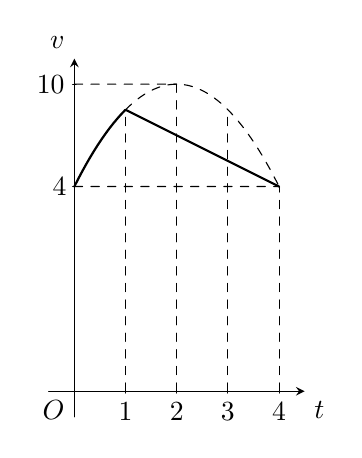
\begin{tikzpicture}[scale=0.65, >=stealth, line join=round, line cap=round,
			declare function={f(\x)=-0.5*(\x)^2+2*(\x)+4;}]
			\def\xt{-0.5} \def\xp{4.5}
			\def\yd{-0.5} \def\yt{6.5}
			\path (0,0) coordinate (O)
			(0,4) coordinate (P0)
			(1,{f(1)}) coordinate (P1)
			(2,{f(2)}) coordinate (P2)
			(3,{f(3)}) coordinate (P3)
			(4,4) coordinate (P4);
			\draw[->] (\xt,0)--(\xp,0) node[below right]{$t$};
			\draw[->] (0,\yd)--(0,\yt) node[above left]{$v$};
			\node[below left] at (O) {$O$};
			\foreach \x in {1,2,3,4} {
				\draw (\x,1pt)--(\x,-1pt) node[below]{$\x$};
			}
			\draw (-1pt,4)--(1pt,4) node[left]{$4$};
			\draw (-1pt,{f(2)})--(1pt,{f(2)});
			\foreach \p in {P1,P2,P3,P4} {
				\draw[dashed] (\p|-0,0) -- (\p);
			}
			\draw[dashed] (0,{f(2)}) node[left]{$10$} -- (P2);
			\draw[dashed] (0,4) -- (P4);
			\draw[dashed, samples=100, domain=1:4] plot (\x,{f(\x)});
			\draw[thick, samples=100, domain=0:1] plot (\x,{f(\x)});
			\draw[thick] (P1) -- (P4);
		\end{tikzpicture}
	}
	\loigiai{
		Trong khoảng thời gian $1$ giờ đầu, đồ thị vận tốc của vật là một đường parabol có phương trình $v=at^2+bt+c$, $(a \ne 0)$ có đỉnh là $I(2;10)$ nên ta có hệ phương trình $$\heva{&c=4\\&4a+2b+c=10\\&-\dfrac{b}{2a}=2} \Leftrightarrow \heva{&a=-\dfrac{3}{2}\\&b=6\\&c=4} \Rightarrow v(t)=-\dfrac{3}{2}t^2+6t+4.$$
		Tại $t=1$, ta có $v=\dfrac{17}{2}$.\\
		Vì khoảng thời gian còn lại, vật chuyển động chậm dần đều nên có phương trình $v(t)=dt+e$, $(d <0)$.\\
		Dựa vào đồ thị, ta có hệ phương trình $\heva{&d+e=\dfrac{17}{2}\\&4d+e=4} \Leftrightarrow \heva{&d=-\dfrac{3}{2}\\&e=10.}$\\
		Vậy vận tốc của vật trong $4$ giờ được biểu thị bởi hàm số $v(t)=\heva{&-\dfrac{3}{2}t^2+6t-4 &&(0 \leq t \leq 1)\\&-\dfrac{3}{2}t+10 &&(1<t \leq 4).}$\\
		Vậy quãng đường vật đi được trong $4$ giờ đó $$s=\displaystyle\int\limits_{0}^{4}v(t)\;\mathrm{d}t=\displaystyle\int\limits_{0}^{1}\left(-\dfrac{3}{2}t^2+6t-4\right)\;\mathrm{d}t+\displaystyle\int\limits_{1}^{4}\left(-\dfrac{3}{2}t+10\right)\;\mathrm{d}t=\dfrac{101}{4}.$$
		Quãng đường $S$ mà vật đi được khoảng $25,3$.
	}
\end{ex}

% #364 | Archive/SP_SauLuoi_2024-2025/Sp_GHKII/data/GHKII/2-TN-DS-TLN-thpt-thuan-thanh-1-2-3-bac-ninh-GHKII-NH24-25.tex | mã gốc 2D4H2-6
\begin{ex}%[Đề thi giữa học kỳ 2 lớp 12 THPT Thuận Thành-Bắc Ninh]%[Nguyễn Tấn Linh]%[2D4H2-6]
	Một quần thể vi khuẩn ban đầu gồm $500$ vi khuẩn, sau đó bắt đầu tăng trưởng. Gọi $P(t)$ là số lượng vi khuẩn của quần thể đó tại thời điểm $t$, trong đó $t$ tính theo ngày ($0 \le t \le 10$). Tốc độ tăng trưởng của quần thể vi khuẩn đó cho bởi hàm số $P'(t) = 150 \sqrt{t}$. Tính số lượng vi khuẩn của quần thể đó sau $9$ ngày.
	\shortans{$3200$}
	\loigiai{
		Số lượng vi khuẩn của quần thể sau $t$ ngày $P(t)=\displaystyle\int150\sqrt{t}\;\mathrm{d}t=100\cdot t\sqrt{t}+C$.\\
		Vì ban đầu quần thể có $500$ vi khuẩn nên $P(0)=500 \Leftrightarrow C=500$.\\
		Vậy $P(t)=100\cdot t\sqrt{t}+500$.\\
		Số lượng vi khuẩn của quần thể sau $9$ ngày $P(9)=3200$ (vi khuẩn).
	}
\end{ex}

% #1750 | Archive/2024/San pham - Tex hoa Lop 12 Chuong trinh moi - Dot 5 (Chuong 5)/Data/Chuong 4/Ket noi tri thuc/KNTT-Chuong4-Ontapchuong-De2.tex | mã gốc 2D4H3-5
\begin{ex}%[2D4H3-5]%[KNTT - Chương 4 - Ôn tập chương - Đề 2]%[Vũ Hồng Toàn]
Trong các mệnh đề sau, chỉ ra mệnh đề đúng, mệnh đề sai.
\choiceTF
{$\displaystyle\int\limits_0^2\left(3x^2-2\mathrm{e}^x\right)\mathrm{\,d}x=6-2\mathrm{e}^2$}
{\True Nước chảy từ đáy của một bồn chứa với tốc độ $k(t)=250-6t$ (lít/phút), trong đó $0\leq t \leq 45$. Lượng nước chảy ra khỏi bồn chứa trong 10 phút đầu tiên bằng 2200 (lít)}
{\True $\displaystyle\int\limits_{\tfrac{\pi}{6}}^{\tfrac{\pi}{4}}\left(\tan ^2x-\cot ^2x\right)\mathrm{\,d}x=a-\dfrac{b}{c} \sqrt{3}$ với $a, b, c \in \mathbb{R}, c \neq 0$ và $\dfrac{b}{c}$ tối giản thì $a+b+c=9$}
{$\displaystyle\int\limits_0^{\tfrac{\pi}{3}}\left|\cos ^2x-\sin x \cos x\right|\mathrm{\,d}x=a+b \pi-c \sqrt{3}$ với $a, b, c \in \mathbb{R}$ thì $a-c+b=\dfrac{5}{6}$}
\loigiai{
\begin{itemchoice}
\itemch Sai.
\allowdisplaybreaks
\begin{eqnarray*}
\displaystyle\int\limits_0^2\big(3 x^2-2 \mathrm{e}^x\big)\mathrm{\,d}x&=&3 \displaystyle\int\limits_0^2 x^2\mathrm{\,d}x-2 \displaystyle\int\limits_0^2 \mathrm{e}^x \mathrm{\,d} x\\&=&x^3\bigg|_0^2-2\mathrm{e}^x\bigg|_0^2=8-\left(2 \mathrm{e}^2-2\right)\\&=&10-2\mathrm{e}^2.
\end{eqnarray*}
\itemch Đúng. Lượng nước chảy ra khỏi bồn chứa trong $10$ phút đầu tiên là
$$
V=\displaystyle\int\limits_0^{10} k(t)\mathrm{\,d} t=\displaystyle\int\limits_0^{10}(250-6 t)\mathrm{\,d}t=\left(250 t-3 t^2\right)\bigg|_0 ^{10}=2200\, \text{(lít)}.
$$
\itemch Đúng. Ta có
\allowdisplaybreaks
\begin{eqnarray*}
\displaystyle\int\limits_{\tfrac{\pi}{6}}^{\tfrac{\pi}{4}}\left(\tan ^2x-\cot ^2x\right)\mathrm{\,d} x&=&\displaystyle\int\limits_{\tfrac{\pi}{6}}^{\tfrac{\pi}{4}}\left(\dfrac{1}{\cos ^2x}-1-\dfrac{1}{\sin ^2x}+1\right)\mathrm{\,d} x\\&=&\displaystyle\int\limits_{\tfrac{\pi}{6}}^{\tfrac{\pi}{4}}\left(\dfrac{1}{\cos ^2x}-\dfrac{1}{\sin ^2x}\right)\mathrm{\,d}x\\
&=&(\tan x+\cot x)\bigg|_{\tfrac{\pi}{6}}^{\tfrac{\pi}{4}}=2-\left(\dfrac{1}{\sqrt{3}}+\sqrt{3}\right)\\&=&2-\dfrac{4}{3} \sqrt{3}.
\end{eqnarray*}
Do đó $a+b+c=9$.
\itemch Sai. $$
\displaystyle\int\limits_0^{\tfrac{\pi}{3}}\left|\cos^2 x-\sin x \cos x\right|\mathrm{\,d}x=\displaystyle\int\limits_0^{\tfrac{\pi}{3}}\big(|\cos x|\cdot|\cos x-\sin x|\big)\mathrm{\,d}x.
$$
Ta có $\cos x > 0$ với mọi $x \in\left[0; \dfrac{\pi}{3}\right]$ và phương trình $\cos x-\sin x=0$ có nghiệm $x=\dfrac{\pi}{4}$ trên đoạn $\left[0; \dfrac{\pi}{3}\right]$.\\
Do đó
\allowdisplaybreaks
\begin{eqnarray*}
\displaystyle\int\limits_0^{\tfrac{\pi}{3}}(|\cos x|\cdot|\cos x-\sin x|)\mathrm{\,d} x&=&\displaystyle\int\limits_0^{\tfrac{\pi}{4}}[\cos x \cdot(\cos x-\sin x)]\mathrm{\,d} x-\displaystyle\int\limits_{\tfrac{\pi}{4}}^{\tfrac{\pi}{3}}[\cos x.(\cos x-\sin x)]\mathrm{\,d}x\\
&=&\displaystyle\int\limits_0^{\tfrac{\pi}{4}}\left(\cos ^2x-\sin x \cos x\right)\mathrm{\,d} x-\displaystyle\int\limits_{\tfrac{\pi}{4}}^{\tfrac{\pi}{3}}\left(\cos ^2x-\sin x \cos x\right)\mathrm{\,d}x\\
&=&\dfrac{1}{2} \displaystyle\int\limits_0^{\tfrac{\pi}{4}}(1+\cos 2x-\sin 2x)\mathrm{\,d}x-\dfrac{1}{2} \displaystyle\int\limits_{\tfrac{\pi}{4}}^{\tfrac{\pi}{3}}((1+\cos 2x-\sin 2x))\mathrm{\,d}x\\
&=&\dfrac{1}{2}\left(x+\dfrac{1}{2} \sin 2x+\dfrac{1}{2} \cos 2x\right)\bigg|_0 ^{\tfrac{\pi}{4}}\\&&-\dfrac{1}{2}\left(x+\dfrac{1}{2} \sin 2x+\dfrac{1}{2} \cos 2x\right)\bigg|_{\tfrac{\pi}{4}} ^{\tfrac{\pi}{3}}\\
&=&\dfrac{\pi}{8}+\dfrac{1}{4}-\left[\dfrac{\pi}{6}+\dfrac{\sqrt{3}}{8}-\dfrac{1}{8}-\left(\dfrac{\pi}{8}+\dfrac{1}{4}\right)\right]\\&=&\dfrac{\pi}{8}+\dfrac{1}{4}-\dfrac{\pi}{6}-\dfrac{\sqrt{3}}{8}+\dfrac{3}{8}+\dfrac{\pi}{8}\\&=&\dfrac{5}{8}+\dfrac{\pi}{12}-\dfrac{\sqrt{3}}{8}.
\end{eqnarray*}
Do đó $a=\dfrac{5}{8}$, $b=\dfrac{1}{12}$, $c=\dfrac{1}{8}$.\\ Vậy $a-c+b=\dfrac{1}{2}-\dfrac{1}{12}=\dfrac{5}{12}$.
\end{itemchoice}
}
\end{ex}

% #1751 | Archive/2024/San pham - Tex hoa Lop 12 Chuong trinh moi - Dot 5 (Chuong 5)/Data/Chuong 4/Ket noi tri thuc/KNTT-Chuong4-Ontapchuong-De2.tex | mã gốc 2D4H3-5
\begin{ex}%[2D4H3-5]%[KNTT - Chương 4 - Ôn tập chương - Đề 2]%[Vũ Hồng Toàn]
Một chiếc cổng có dạng là một parabol $(P)$ có kích thước như hình vẽ, biết chiều cao cổng bằng chiều rộng của cổng và bằng $4$\,m (Tham khảo Hình 1). Người ta thiết kế cửa đi là một hình chữ nhật $CDEF$, phần còn lại dùng để trang trí. Biết chi phí phần tô đậm là $1\,000\,000$\,đồng/m$^2$.
\begin{center}
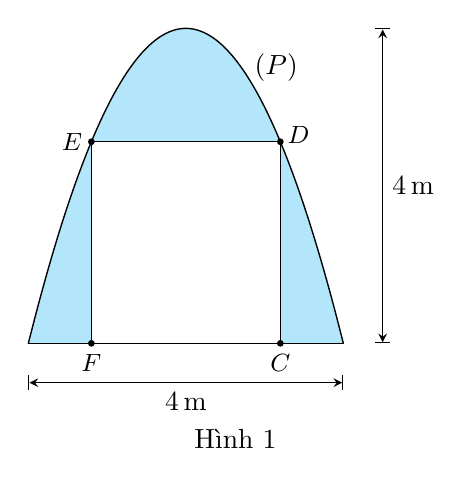
\begin{tikzpicture}[scale=1, line join=round, line cap=round, >=stealth,
declare function={cr=1.2;f(\x)=-(\x)^2 + 4; xmin=-3; xmax=3.5; ymin=-1; ymax=4.2;}]
%\draw[color=gray!50,thin] (xmin,ymin) grid (xmax,ymax);
\path (cr,0) coordinate (C)
(cr,{f(cr)})coordinate (D)
(-cr,{f(-cr)})coordinate (E)
(-cr,0) coordinate (F);
\fill[cyan!30] (-2,0)--	plot[domain=-2:2] (\x, {f(\x)})--cycle;
\fill[white] (C)--(D)--(E)--(F)--cycle;
% Vẽ đồ thị hàm số
\draw[smooth, samples=100, line width=.5] plot[domain=-2:2] (\x, {f(\x)});
\draw (-2,0)--(2,0) (C)--(D)--(E)--(F) (0.75,3.5)node[right]{$(P)$};
\draw[|<->|](-2,-0.5)--(2,-0.5)node[pos=0.5, below]{$4$\,m};
\draw[|<->|](2.5,0)--(2.5,4)node[pos=0.5, right]{$4$\,m};
\foreach \x/\goc in {C/-90,D/20,E/180,F/-90}{
\draw[fill] (\x) circle (1pt) node[shift={(\goc:7pt)},font=\small]{$\x$};
}
\path (current bounding box.south) node[below]{Hình 1};
\end{tikzpicture}
\hspace{1.5cm}
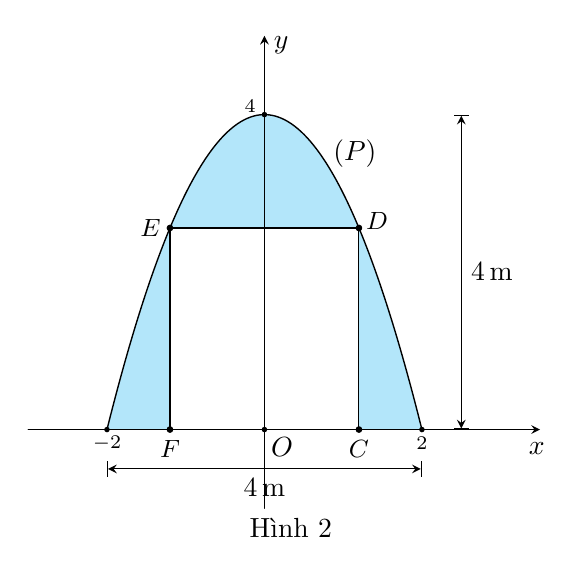
\begin{tikzpicture}[scale=1, line join=round, line cap=round, >=stealth, declare function={cr=1.2;f(\x)=-(\x)^2 + 4; xmin=-3; xmax=3.5; ymin=-1; ymax=5;}]
\path (cr,0) coordinate (C)
(cr,{f(cr)})coordinate (D)
(-cr,{f(-cr)})coordinate (E)
(-cr,0) coordinate (F);
\fill[cyan!30] (-2,0)--	plot[domain=-2:2] (\x, {f(\x)})--cycle;
\fill[white] (C)--(D)--(E)--(F)--cycle;
% Trục toạ độ
\draw[->] (xmin,0)--(xmax,0) node[shift={(-100:7pt)},font=\normalsize]{$ x $};
\draw[->] (0,ymin)--(0,ymax) node[shift={(-30:7pt)},font=\normalsize]{$ y $};
\fill (0,0) circle (1pt) node[shift={(-45:9pt)},font=\normalsize]{$ O $};
% Vẽ đồ thị hàm số
\draw[smooth, samples=100, line width=.5] plot[domain=-2:2] (\x, {f(\x)});
% Các điểm trên trục x và y
\foreach \x/\goc in {-2/-90,2/-90}{
\fill (\x,0) circle (1pt) node[shift={(\goc:5pt)},font=\scriptsize]{$\x$};}

\foreach \y/\goc in {4/150}{
\fill (0,\y) circle (1pt) node[shift={(\goc:6pt)},font=\scriptsize]{$\y$};}
\draw (-2,0)--(2,0) (C)--(D)--(E)--(F) (0.75,3.5)node[right]{$(P)$};
\draw[|<->|](-2,-0.5)--(2,-0.5)node[pos=0.5, below]{$4$\,m};
\draw[|<->|](2.5,0)--(2.5,4)node[pos=0.5, right]{$4$\,m};
\foreach \x/\goc in {C/-90,D/20,E/180,F/-90}{
\draw[fill] (\x) circle (1pt) node[shift={(\goc:7pt)},font=\small]{$\x$};
}
\path (current bounding box.south) node[below]{Hình 2};
\end{tikzpicture}
\end{center}
\choiceTF
{\True Chọn hệ trục tọa độ $Oxy$, như Hình 2 thì phương trình của đường cong $(P)$ cánh cổng là $y=f(x)=-x^2+4$}
{\True Nếu chiều cao cửa đi là $CD=2$\,m thì chiều rộng của cửa là $CF=2\sqrt{2}$\,m}
{Nếu chiều cao cửa đi là $CD=2$\,m thì chi phí để trang trí phần tô đậm là $\dfrac{32-6\sqrt{2}}{3}$\,(triệu đồng)}
{\True Số tiền ít nhất dùng để trang trí phần tô đậm (làm tròn đến hàng nghìn đồng) là $4\,508\,000$\,(đồng)}
\loigiai{
\begin{itemchoice}
\itemch Đúng. Từ hình vẽ, ta có parabol $(P)$ có dạng $y=a x^2+b x+c; a, b, c \in \mathbb{R}$.\\
Do $(P)$ có đồ thị là parabol có đỉnh $(0;4)$ và đi qua điểm có tọa độ là $(2; 0)$ nên \[\heva{&b=0\\& c=4\\& 4a+2b+c=0}\heva{&a=-1\\& b=0\\& c=4.}\]
Vậy $(P)$ có phương trình $y=-x^2+4$.
\itemch Đúng. Theo giả thiết điểm $D$ thuộc đồ thị $(P)$ có tung độ bằng $2$ suy ra hoành độ là nghiệm phương trình \[-x^2+4=2\Leftrightarrow x=\pm \sqrt{2}.\]
Theo đồ thị điểm $D$ có hoành độ dương nên $D(\sqrt{2};2)$.\\
Chiều rộng của cửa là $CF=2\cdot OD=2\sqrt{2}$\,m.
\itemch Sai. Diện tích của $(P)$ tạo với trục hoành là \[S=\displaystyle\int_{-2}^2\left(-x^2+4\right)\mathrm{\,d} x=\dfrac{32}{3}\text{m}^2.\]
Diện tích hình chữ nhật $CDEF$ là $S_{CDEF}=2\cdot 2\sqrt{2}=4\sqrt{2}$.\\
Diện tích cần trang trí là $S_1=S-S_{CDEF}=\dfrac{32}{3}-4\sqrt{2}=\dfrac{32-12\sqrt{2}}{3}$.\\
Chi phí để trang trí phần tô đậm là $\left(\dfrac{32-12\sqrt{2}}{3}\right) \cdot 1\,000\,000$\,(đồng).
\itemch Đúng. Ta có, diện tích của $(P)$ tạo với trục hoành là $S=\displaystyle\int_{-2}^2\left(-x^2+4\right)\mathrm{\,d} x=\dfrac{32}{3}$\,m$^2$.\\
Ta gọi điểm $C(a; 0) \Rightarrow D\left(a;-a^2+4\right); 0< a < 2$.\\
Do đó, diện tích của hình chữ nhật $CDEF$ là $S_{CDEF}=2a\left(4-a^2\right)=8a-2a^3$.\\
Theo đề bài, để phần trang trí, có chi phí nhỏ nhất thì diện tích của hình chữ nhật $CDEF$ đạt giá trị lớn nhất.\\
Do cổng chào đối xứng qua trục tung nên ta đặt: $g(a)=\dfrac{S_{CDEF}}{2}=4a-a^3,0< a < 2$.
$\Rightarrow g'(a)=4-3a^2\Rightarrow g'(a)=0\Rightarrow a=\dfrac{2\sqrt{3}}{3}$.\\
Ta có, bảng biến thiên\\
\centerline{

\begin{tikzpicture}
\tkzTabInit
{$a$/0.7, $g'(a)$/0.7, $g(a)$/2.1} % Khai báo tiêu đề và độ rộng cột
{$0$, $\tfrac{2\sqrt{3}}{3}$, $2$} % Giá trị trên trục
\tkzTabLine{,+,0,-} % Dấu của đạo hàm
\tkzTabVar{-/ , +/$\tfrac{16\sqrt{3}}{9}$, -/ } % Giá trị của hàm số
\end{tikzpicture}
}
Dựa vào bảng biến thiên, suy ra diện tích hình chữ nhật $CDEF$ đạt giá trị lớn nhất là $\dfrac{32\sqrt{3}}{9}$\,m$^2$.\\
Vậy diện tích nhỏ nhất của phần dùng để trang trí là $\dfrac{96-32\sqrt{3}}{9}$\,m$^2$.\\
Do đó, số tiền ít nhất dùng để trang trí phần tô đậm là\\
$\left(\dfrac{96-32\sqrt{3}}{9}\right) \cdot 1\,000\,000=4\,508\,263{,}795\approx 4\,508\,000$\,đồng.
\end{itemchoice}
}
\end{ex}

% #1755 | Archive/2024/San pham - Tex hoa Lop 12 Chuong trinh moi - Dot 5 (Chuong 5)/Data/Chuong 4/Ket noi tri thuc/KNTT-Chuong4-Ontapchuong-De2.tex | mã gốc 2D4V2-6
\begin{ex}%[2D4V2-6]%[KNTT - Chuong 4 - On tap chuong - De 2]%[Trần Hưng]
	Một ô tô đang chạy với vận tốc $20$ ($\text{m/s}$) thì người ta nhìn thấy một chướng ngại vật nên đạp phanh. Từ thời điểm đó, ô tô chuyển động chậm dần đều với vận tốc $v(t)=-2t+20$ ($\text{m/s}$) trong đó $t$ là thời gian (tính bằng giây) kể từ lúc đạp phanh. Quãng đường mà ô tô đi được trong $15$ giây cuối bằng bao nhiêu?
	\shortans{$200$}
	\loigiai{
		Khi ô tô dừng lại, ta có $v(t)=0\Rightarrow-2t+20=0\Leftrightarrow t=10$ (s).\\
		Quãng đường ô tô đi được từ lúc đạp phanh đến khi dừng lại là\\
		$s=\displaystyle\int\limits _{0}^{10}v(t)\mathrm{\, d}t=\displaystyle\int\limits _{0}^{10}(-2t+20)\mathrm{\, d}t=\left(-t^2+20t\right)\bigg|_{0}^{10}=100$ (m).\\
		Trong $5$ giây trước đó, ô tô vẫn đi với vận tốc $20$ ($\text{m/s}$) nên quãng đường ô tô đi được trong $5$ giây này là $5\cdot 20=100$ (m).\\
		Vậy quãng đường mà ô tô đi được trong $15$ giây cuối bằng $100+100=200$ (m).
	}
\end{ex}

% #1756 | Archive/2024/San pham - Tex hoa Lop 12 Chuong trinh moi - Dot 5 (Chuong 5)/Data/Chuong 4/Ket noi tri thuc/KNTT-Chuong4-Ontapchuong-De2.tex | mã gốc 2D4V3-5
\begin{ex}%[2D4V3-5]%[KNTT - Chuong 4 - On tap chuong - De 2]%[Trần Hưng]
	\immini[thm]{
		Một cốc rượu có hình dạng tròn xoay (không kể phần chân đế) có kích thước như hình vẽ. Thiết diện dọc của cốc (bổ dọc cốc thành $2$ phần bằng nhau) là một đường Parabol. Tính
		thể tích rượu tối đa mà cốc có thể chứa được (làm tròn đến hàng đơn vị, đơn vị đo thể tích là $\text{cm}^3$)
	}{
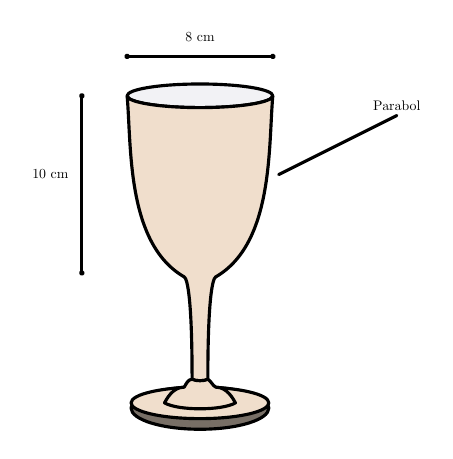
\begin{tikzpicture}[line join=round, line cap=round,scale=0.5,transform shape,line width=.4mm]
	\definecolor{almond}{rgb}{0.94, 0.87, 0.8}%màu ly
	\definecolor{anti-flashwhite}{rgb}{0.95, 0.95, 0.96}%màu miệng ly
	\tikzset{co_vat/.pic={
			\path 
			(1.85,4)coordinate (A)			
			(-1.85,4) coordinate (B)	
			(-3,3)coordinate (C)
			(-3,-1.5)coordinate (D)					
			;
			\draw (A)--(B) (C)--(D);
			\foreach\p in {A,B,C,D}
			{\draw[fill=black](\p) circle (1pt);}	
			\node at (-3.8,1) {$10$ cm};
			\node at (0,4.5) {$8$ cm};
			\draw (2,1)--(5,2.5) node[above] {Parabol};			
			\draw[fill=almond!50!black] (1.75,-4.93)  arc (0:360:1.75 cm and .54cm);
			\draw[fill=almond] (1.75,-4.8)  arc (0:360:1.75 cm and .4cm);			
			\draw[fill=anti-flashwhite] (1.85,3)  arc (0:360:1.85 cm and .3cm);
			\draw[fill=almond] (1.85,3)
			..controls +(-95:1.3) and +(30:1.7) ..(.4,-1.6) 
			..controls +(-150:.1) and +(90:2) ..(.2,-4.2) 
			..controls +(-150:.1) and +(-30:.1) ..(-.2,-4.2) 
			..controls +(90:2) and +(-30:.1) ..(-.4,-1.6) 
			..controls +(150:1.7) and +(-85:1.3) ..(-1.85,3)
			arc (-180:0:1.85 cm and .3cm);
			;
			\draw[fill=almond] (.2,-4.2) 
			..controls +(-150:.1) and +(-30:.1) ..(-.2,-4.2) 
			..controls +(180:.1) and +(60:.1) ..(-.4,-4.4) 
			..controls +(180:.3) and +(60:.1) ..(-.9,-4.8) 
			..controls +(-30:.4) and +(-150:.4) ..(.9,-4.8) 
			..controls +(120:.1) and +(0:.3) ..(.4,-4.4)
			..controls +(150:.1) and +(-30:.1) ..(.2,-4.2) 
			;			
	}}	
	\path
	(0,0)pic[scale=1]{co_vat};	
\end{tikzpicture}}
	\shortans{$251$}
	\loigiai{
		\begin{center}
			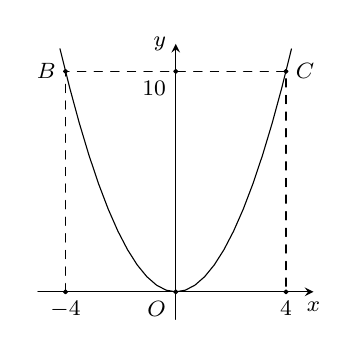
\begin{tikzpicture}[scale=.7, font=\footnotesize, line join=round, line cap=round, >=stealth]
				\draw [->] (-2.5,0) -- (2.5,0) node[below]{$x$};
				\draw [->] (0,-.5) -- (0,4.5) node[left]{$y$};
				\draw (0,0) node[below left]{$O$} circle(1pt);
				\draw plot[domain=-2.1:2.1](\x,{(\x)^2});
				\draw[dashed] (-2,0)--(-2,4)--(2,4)--(2,0);
				\draw[fill=black] (-2,0) circle(1pt) node[below]{$-4$};
				\draw[fill=black] (2,0) circle(1pt) node[below]{$4$};
				\draw[fill=black] (0,4) circle(1pt) node[below left]{$10$};
				\draw[fill=black] (-2,4) circle(1pt) node[left]{$B$};
				\draw[fill=black] (2,4) circle(1pt) node[right]{$C$};
			\end{tikzpicture}
		\end{center}
		Parabol có phương trình $y=\dfrac{5}{8}x^2\Leftrightarrow x^2=\dfrac{8}{5}y$.\\
		Thể tích tối đa cốc\\
		$V=\pi \displaystyle\int\limits _{0}^{10}\left(\dfrac{8}{5}y\right)\mathrm{\, d}y\approx 251{,}33$.
	}
\end{ex}

% #1757 | Archive/2024/San pham - Tex hoa Lop 12 Chuong trinh moi - Dot 5 (Chuong 5)/Data/Chuong 4/Ket noi tri thuc/KNTT-Chuong4-Ontapchuong-De2.tex | mã gốc 2D4V3-2
\begin{ex}%[2D4V3-2]%[KNTT - Chuong 4 - On tap chuong - De 2]%[Trần Hưng]
	\immini[thm]{
		Một chi tiết máy hình đĩa tròn có dạng như hình vẽ bên nhận $AB$, $CD$ làm các trục đối xứng. Người ta cần phủ sơn cả hai mặt của chi tiết. Biết rằng đường tròn lớn có bán kính $5$ dm, các đường tròn nhỏ đều có bán kính bằng $2$ dm, $AB=CD=4$ dm và chi phí sơn là $100\,000$ đồng /$\text{m}^2$. Tính chi phí $x$ (nghìn đồng) để sơn hoàn thiện chi tiết máy (làm tròn đến sau dấu phẩy 1 chữ số).
	}{
		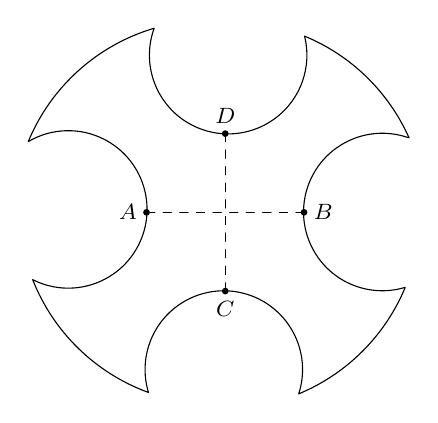
\begin{tikzpicture}[scale=1, font=\footnotesize, line join=round, line cap=round, >=stealth]
		\draw[fill=black]  (-1,0) circle(1pt) node[left]{$A$};
		\draw[fill=black]  (1,0) circle(1pt) node[right]{$B$};
		\draw[fill=black]  (0,-1) circle(1pt) node[below]{$C$};
		\draw[fill=black]  (0,1) circle(1pt) node[above]{$D$};
		\draw (2.32,0.95) arc (71:286.92:1) arc(-22.5:-67.5:2.5)  arc(-18:196.92:1) arc(-110:-158.5:2.5) arc(-116.92:120.6:1) arc(-202.5:-253.5:2.5) arc(-200:14:1) arc(-292.5:-336:2.5);
		\draw[dashed] (-1,0)--(1,0) (0,-1)--(0,1);
	\end{tikzpicture}
}
	\shortans{$79{,}5$ }
	\loigiai{
		\begin{center}
			\begin{tikzpicture}[scale=1, font=\footnotesize, line join=round, line cap=round, >=stealth]
				\draw [->] (-3,0) -- (3,0) node[below]{$x$};
				\draw [->] (0,-3) -- (0,3) node[left]{$y$};
				\draw (0,0) node[below left]{$O$} circle(1pt);
				\draw[fill=black]  (-1,0) circle(1pt) node[above right]{$A$};
				\draw[fill=black]  (1,0) circle(1pt) node[above left]{$B$};
				\draw[fill=black]  (0,-1) circle(1pt) node[below right]{$C$};
				\draw[fill=black]  (0,1) circle(1pt) node[above left]{$D$};
				\draw[fill=black]  (2,0) circle(1pt) node[below]{$I$};
				\draw[fill=black]  (2,0) circle(1pt) node[above]{$4$};
				\draw[fill=black]  (2.5,0) node[above right]{$5$};	
				\draw (2.32,0.95) arc (71:286.92:1) arc(-22.5:-67.5:2.5)  arc(-18:196.92:1) arc(-110:-158.5:2.5) arc(-116.92:120.6:1) arc(-202.5:-253.5:2.5) arc(-200:14:1) arc(-292.5:-336:2.5) ;
				\fill[pattern=north east lines,opacity=1, line width = 1.2pt] (2.32,0.95) arc (71:286.92:1) circle(1pt) node[below right, black]{$F$} arc(-22.5:20.5:2.6);
				\draw[fill=black]  (2.32,0.95) circle(1pt) node[above]{$E$};
			\end{tikzpicture}
		\end{center}
		Chọn hệ toạ độ $Oxy$ sao cho $O$ trùng với giao điểm của $AB$ và $CD$; các tia lần lượt trùng với các tia $OB$, $OD$. \\
		Ta có:\\
		Phương trình đường tròn lớn tâm $O$ là: $x^2+y^2=25\Leftrightarrow y=\pm\sqrt{25-x^2}$.\\
		Phương trình đường tròn nhỏ tâm $I$ là: $(x-4)^2+y^2=4\Leftrightarrow y=\pm\sqrt{4-(x-4)^2}$.\\
		Phương trình hoành độ giao điểm của 2 đường tròn là: $4-(x-4)^2=25-x^2\Leftrightarrow x=\dfrac{37}{8}$.
		Gọi $S$, $S_t$, $S'$ lần lượt là diện tích một mặt của chi tiết, diện tích đường tròn tâm $O$ và diện tích phần gạch sọc.\\
		Ta có: $S=S_t-4S'=25\pi -4\cdot \left(2\displaystyle\int\limits _2^{\tfrac{37}{8}}\sqrt{4-(x-4)^2}\mathrm{\, d}x+2\displaystyle\int\limits _{\tfrac{37}{8}}^5\sqrt{25-x^2}\mathrm{\, d}x\right)$.\\
		Vậy chi phí để sơn hoàn thiện chi tiết máy là: $x=S\cdot 2\cdot 1\,000\approx 79{,}5$ (nghìn đồng).
	}
\end{ex}

% #1763 | Archive/2024/San pham - Tex hoa Lop 12 Chuong trinh moi - Dot 5 (Chuong 5)/Data/Chuong 4/Canh dieu/CD-Chuong4-Ontapchuong-De3.tex | mã gốc 2D4H2-6
\begin{ex}%[2D4H2-6] %[Cánh diều - Chương 4 - Ôn tập chương 3 - Đề 3]%[Thầy Tú TLH]%câu 15
	Một ô tô đang chạy với vận tốc $16$ m/s thì người lái xe bất ngờ phát hiện chướng ngại vật trên đường cách đó $50$ m. Người lái xe phản ứng một giây sau đó đạp phanh khẩn cấp. Từ thời điểm đó, ô tô chuyển động chậm dần đều với vận tốc $v(t)=-5t+15$, trong đó là khoảng thời gian tính bằng giây, kể từ lúc bắt đầu đạp phanh. Gọi $s(t)$ là quãng đường ô tô đi được trong $t$ giây kể từ lúc đạp phanh.	
	\choiceTF
	{Công thức biểu diễn hàm số $s(t)$ là $s(t)=-\dfrac{5t^2}{2}+15t+16$}
	{\True Thời gian kể từ khi ô tô đạp phanh đến khi dừng hẳn bằng $3$ giây}
	{Kể từ lúc đạp phanh đến khi dừng hẳn, ô tô còn di chuyển được quãng đường là $38{,}5$ m}
	{\True Xe ô tô không va chạm với chướng ngại}
	\loigiai
	{
		% Lời giải chung
		\begin{itemchoice}
			\itemch Sai. Ta có $s(t)=\displaystyle\int \left(-5t+15\right)\mathrm{\,d}t=-\dfrac{5t^2}{2}+15t+C$.\\
			Do $s(0)=0$ nên $C=0$.\\
			Vậy $s(t)=-\dfrac{5t^2}{2}+15t$.
			\itemch Đúng. Ô tô dừng hẳn khi $v(t)=0$ $\Leftrightarrow-5t+15=0\Leftrightarrow t=3$.
			\itemch Sai. Quãng đường ô tô di chuyển được từ lúc đạp phanh đến khi dừng hẳn là\\
			$s(3)=\dfrac{-5\cdot 9}{2}+15\cdot 3=22{,}5$ (m). 
			\itemch Đúng. Do trước khi đạp phanh tài xế còn phản ứng một giây nên kể từ lúc phát hiện chướng ngại đến khi dừng hẳn ô tô đi được quãng đường là\\ $16+22{,}5=38{,}5$ m.\\
			Do đó ô tô không va chạm với chướng ngại vật.
		\end{itemchoice}
	}
\end{ex}

% #1908 | Archive/2024/TaiLieuGiangDay/3. K12 - 4in1 - Thongke/data/2. Bai1-Dang2-KhoangTuPhanVi.tex | mã gốc 2D4V1-3
\begin{ex}[Mức độ 3]%[2D4V1-3]
	Bảng mẫu số liệu ghép nhóm thống kê mức lương của một công ty (đơn vị: triệu đồng) được cho như sau:
	\begin{center}
		{\setlength\extrarowheight{2pt}
			\begin{tabular}{|>{\centering\arraybackslash}m{3cm}|*{6}{>{\centering\arraybackslash}m{1.8cm}|}}
				\hline 
				Nhóm & $[10;15)$ & $[15;20)$ & $[20;25)$ & $[25;30)$ & $[30;35)$ & $[35;40)$\\
				\hline 
				Tần số & $15$ & $18$ & $10$ & $10$ & $5$ & $2$\\
				\hline 
		\end{tabular}}
	\end{center}
	Từ bảng mẫu số liệu ghép nhóm nói trên. Ta có
	\choiceTF[t]
	{Cỡ mẫu là $n=100$}
	{\True Tần số tích lũy của nhóm $[30;35)$ là $58$}
	{Trung vị của mẫu số liệu ghép nhóm là $M_e\in (24;25)$}
	{\True Khoảng tứ phân vị của mẫu số liệu ghép nhóm là $\Delta_Q=11$}
	\loigiai{
		Ta có bảng tần số tích lũy của mẫu số liệu như sau
		\begin{center}
			{\setlength\extrarowheight{2pt}
				\begin{tabular}{|>{\centering\arraybackslash}m{3cm}|*{6}{>{\centering\arraybackslash}m{1.8cm}|}}
					\hline 
					Nhóm & $[10;15)$ & $[15;20)$ & $[20;25)$ & $[25;30)$ & $[30;35)$ & $[35;40)$\\
					\hline 
					Tần số & $15$ & $18$ & $10$ & $10$ & $5$ & $2$\\
					\hline 
					Tần số tích lũy & $15$ & $33$ & $43$ & $53$ & $58$ & $60$\\
					\hline 
			\end{tabular}}
		\end{center}
		\begin{itemchoice}
			\itemch Cỡ mẫu là $n=60$.
			\itemch Tần số tích lũy của nhóm $[30;35)$ là $58$.
			\itemch Vì $\dfrac{n}{2}=30$ nên nhóm chứa trung vị $M_e$ là nhóm $[15;20)$, suy ra
			$$M_e= Q_2= 15+\dfrac{30-15}{18}\cdot 5 = \dfrac{115}{6} \approx 19{,}2.$$
			\itemch Vì $\dfrac{n}{4}=15$ nên nhóm chứa $Q_1$ là nhóm $[10;15)$, suy ra $Q_1= 10+\dfrac{15-0}{15}\cdot 5 = 15$.\\
			Vì $\dfrac{3n}{4}=45$ nên nhóm chứa $Q_3$ là nhóm $[25;30)$, suy ra $Q_3= 25+\dfrac{45-43}{10}\cdot 5 = 26$.\\
			Vậy khoảng tứ phân vị của mẫu số liệu ghép nhóm đã cho là $\Delta_Q=Q_3-Q_1=11$.
	\end{itemchoice}}
\end{ex}

% #1909 | Archive/2024/TaiLieuGiangDay/3. K12 - 4in1 - Thongke/data/2. Bai1-Dang2-KhoangTuPhanVi.tex | mã gốc 2D4V1-3
\begin{ex}[Mức độ 3]%[2D4V1-3]
	Bảng sau thống kê tổng lượng mưa (đơn vị: mm) đo được vào tháng 7 từ năm 2002 đến 2021 tại một trạm quan trắc đặt ở Cà Mau.
	\begin{center}
		\begin{tabular}{|c|c|c|c|c|c|c|c|c|c|}
			\hline
			$341{,}4$ & $187{,}1$ & $242{,}2$ & $522{,}9$ & $251{,}4$ & $432{,}2$ & $200{,}7$ & $388{,}6$ & $258{,}4$ & $288{,}5$ \\
			\hline
			$298{,}1$ & $413{,}5$ & $413{,}5$ & $332$ & $421$ & $475$ & $400$ & $305$ & $520$ & $147$ \\
			\hline
		\end{tabular}\\
		(Nguồn: Tổng cục Thống kê)
	\end{center}
	Chia mẫu số liệu trên thành $4$ nhóm lần lượt là $[140;240)$, $[240;340)$, $[340;440)$ và $[440;540)$.
	\choiceTF[t]
	{Cỡ mẫu là $n=18$}
	{\True Tần số của nhóm $[240;340)$ là $7$}
	{\True Tứ phân vị $Q_3$ của mẫu số liệu ghép nhóm là $\dfrac{2880}{7}$}
	{Khoảng biến thiên của mẫu số liệu ghép nhóm là $162{,}35$}
	\loigiai
	{Ta có bảng tần số tích lũy của mẫu số liệu ghép nhóm như sau:
		\begin{center}
			{\setlength\extrarowheight{2pt}
				\begin{tabular}{|>{\centering\arraybackslash}m{3cm}|*{4}{>{\centering\arraybackslash}m{2cm}|}}
					\hline 
					Nhóm & $[140;240)$ & $[240;340)$ & $[340;440)$ & $[440;540)$ \\
					\hline 
					Tần số & $3$ & $7$ & $7$ & $3$ \\
					\hline 
					Tần số tích lũy & $3$ & $10$ & $17$ & $20$ \\
					\hline 
			\end{tabular}}
		\end{center}
		\begin{itemchoice}
			\itemch Cỡ mẫu là $n=20$.
			\itemch Tần số của nhóm $[240;340)$ là $7$.
			\itemch Vì $\dfrac{3n}{4}=15$ nên nhóm chứa $Q_3$ là nhóm $[340;440)$, suy ra
			$$Q_3=340+\dfrac{15-10}{7}\cdot 100=\dfrac{2880}{7}.$$
			\itemch Vì $\dfrac{n}{4}=5$ nên nhóm chứa $Q_1$ là nhóm $[240;340)$, suy ra
			$$Q_1=240+\dfrac{5-3}{7}\cdot 100=\dfrac{1880}{7}.$$
			Vậy khoảng tứ phân vị của mẫu số liệu ghép nhóm là $$\Delta_Q=Q_3-Q_1 = \dfrac{2880}{7}-\dfrac{1880}{7}=\dfrac{1000}{7} \approx 142{,}86$$
	\end{itemchoice}}
\end{ex}

% #1910 | Archive/2024/TaiLieuGiangDay/3. K12 - 4in1 - Thongke/data/2. Bai1-Dang2-KhoangTuPhanVi.tex | mã gốc 2D4V1-3
\begin{ex}[Mức độ 3]%[2D4V1-3]
	Kết quả đo chiều cao của $100$ cây keo 3 năm tuổi tại một nông trường được cho ở bảng sau
	\begin{center}
		{\setlength\extrarowheight{2pt}
			\begin{tabular}{|>{\centering\arraybackslash}m{3cm}|*{5}{>{\centering\arraybackslash}m{2cm}|}}
				\hline
				Chiều cao (m) & $[8{,}4;8{,}6)$ & $[8{,}6;8{,}8)$ & $[8{,}8;9{,}0)$ & $[9{,}0;9{,}2)$ & $[9{,}2;9{,}4)$ \\
				\hline
				Số cây & $5$ & $12$ & $25$ & $44$ & $14$ \\
				\hline
		\end{tabular}}
	\end{center}
	\choiceTF[t]
	{Khoảng biến thiên của mẫu số liệu ghép nhóm bằng $9$}
	{\True Số trung bình cộng của mẫu số liệu ghép nhóm đã cho là $9$}
	{Trung vị của mẫu số liệu ghép nhóm là $M_e=9{,}1$}
	{\True Khoảng tứ phân vị của mẫu số liệu ghép nhóm bằng $0{,}286$}
	\loigiai
	{Ta có bảng tần số tích lũy của mẫu số liệu ghép nhóm đã cho như sau:
		\begin{center}
			{\setlength\extrarowheight{2pt}
				\begin{tabular}{|>{\centering\arraybackslash}m{3.5cm}|*{5}{>{\centering\arraybackslash}m{1.9cm}|}}
					\hline
					Nhóm & $[8{,}4;8{,}6)$ & $[8{,}6;8{,}8)$ & $[8{,}8;9{,}0)$ & $[9{,}0;9{,}2)$ & $[9{,}2;9{,}4)$ \\
					\hline
					Giá trị đại diện & $8{,}5$ & $8{,}7$ & $8{,}9$ & $9{,}1$ & $9{,}3$ \\
					\hline
					Tần số & $5$ & $12$ & $25$ & $44$ & $14$ \\
					\hline
					Tần số tích lũy & $5$ & $17$ & $42$ & $86$ & $100$ \\
					\hline
			\end{tabular}}
		\end{center}
		Ta có cỡ mẫu $n=100$.
		\begin{itemchoice}
			\itemch Khoảng biến thiên của mẫu số liệu là $R=9{,}4-8{,}4=1$.\\
			\itemch Số trung bình cộng của mẫu số liệu ghép nhóm là
			$$\overline{x}=\dfrac{5\cdot 8{,}5 + 12\cdot 8{,}7 + 25\cdot 8{,}9 + 44\cdot 9{,}1 + 14\cdot 9{,}3}{100} =9.$$
			\itemch Vì $\dfrac{n}{2}=50$ nên nhóm chứa trung vị $M_e$ là nhóm $[9{,}0;9{,}2)$, suy ra
			$$M_e=Q_2 = 9{,}0 + \dfrac{50-42}{44}\cdot 0{,}2 = \dfrac{497}{55} \approx 9{,}04.$$
			\itemch Vì $\dfrac{n}{4}=25$ nên nhóm chứa $Q_1$ là nhóm $[8{,}8;9{,}0)$, suy ra
			$$Q_1 = 8{,}8 +\dfrac{25-17}{25}\cdot 0{,}2 = \dfrac{1108}{125} = 8{,}864.$$
			Vì $\dfrac{3n}{4}=75$ nên nhóm chứa $Q_3$ là nhóm $[9{,}0;9{,}2)$, suy ra
			$$Q_3=9{,}0+\dfrac{75-42}{44}\cdot 0{,}2 = \dfrac{183}{20}=9{,}15.$$
			Vậy khoảng tứ phân vị của mẫu số liệu ghép nhóm là $\Delta_Q=Q_3-Q_1=0{,}286$.
	\end{itemchoice}}
\end{ex}

% #1911 | Archive/2024/TaiLieuGiangDay/3. K12 - 4in1 - Thongke/data/2. Bai1-Dang2-KhoangTuPhanVi.tex | mã gốc 2D4V1-3
\begin{ex}[Mức độ 3]%[2D4V1-3]
	Thống kê số thẻ vàng của mỗi câu lạc bộ trong giải ngoại hạng Anh mùa giải $2021-2022$ cho kết quả sau:	
	\begin{center}
		{\setlength\extrarowheight{2pt}
			\begin{tabular}{|>{\centering\arraybackslash}m{3.5cm}|*{7}{>{\centering\arraybackslash}m{1.6cm}|}}
				\hline
				Nhóm & $[40;50)$ & $[50;60)$ & $[60;70)$ & $[70;80)$ & $[80;90)$ & $[90;100)$ & $[100;110)$ \\
				\hline
				Tần số & $2$ & $5$ & $7$ & $5$ & $0$ & $0$ & $1$ \\
				\hline
		\end{tabular}}
		\begin{flushright}
			(Theo  \textit{premierleague.com})
		\end{flushright} 	
	\end{center}
	\choiceTF[t]
	{\True Khoảng biến thiên của mẫu số liệu ghép nhóm là $R=70$}
	{Nhóm $[100;110)$ là nhóm có tần số lớn nhất}
	{\True Trung vị của bảng số liệu ghép nhóm (kết quả làm tròn đến hàng đơn vị) là $M_e=64$}
	{\True Khoảng tứ phân vị của mẫu số liệu ghép nhóm là $\Delta_Q=6$}
	\loigiai{
		Ta có bảng tần số tích lũy của mẫu số liệu ghép nhóm như sau:
		\begin{center}
			{\setlength\extrarowheight{2pt}
				\begin{tabular}{|>{\centering\arraybackslash}m{3.5cm}|*{7}{>{\centering\arraybackslash}m{1.6cm}|}}
					\hline
					Nhóm & $[40;50)$ & $[50;60)$ & $[60;70)$ & $[70;80)$ & $[80;90)$ & $[90;100)$ & $[100;110)$ \\
					\hline
					Tần số & $2$ & $5$ & $7$ & $5$ & $0$ & $0$ & $1$ \\
					\hline
					Tần số tích lũy & $2$ & $7$ & $14$ & $19$ & $19$ & $19$ & $20$ \\
					\hline
			\end{tabular}}
		\end{center}
		Cỡ mẫu $n=20$.
		\begin{itemchoice}
			\itemch Khoảng biến thiên của mẫu số liệu ghép nhóm là $R=110-40=70$.
			\itemch Nhóm $[60;70)$ là nhóm có tần số lớn nhất.
			\itemch Vì $\dfrac{n}{2}=10$ nên nhóm chứa trung vị $M_e$ là nhóm $[60;70)$, suy ra 
			$$M_e=Q_2 = 60+\dfrac{10-7}{7}\cdot 10 = \dfrac{450}{7} \approx 64.$$
			\itemch
			Vì $\dfrac{n}{4}=5$ nên nhóm chứa $Q_1$ là nhóm $[50;60)$, suy ra $Q_1 = 50+\dfrac{5-2}{5}\cdot 10 = 56$.\\
			Lại có $\dfrac{3n}{4}=15$ nên nhóm chứa $Q_3$ là nhóm $[70;80)$, suy ra $Q_3 = 60+\dfrac{15-14}{5}\cdot 10 = 62$.\\
			Vậy khoảng tứ phân vị của mẫu số liệu ghép nhóm là $\Delta_Q = Q_3-Q_1 = 62-56 = 6$.			
		\end{itemchoice}
	}
\end{ex}

% #1912 | Archive/2024/TaiLieuGiangDay/3. K12 - 4in1 - Thongke/data/2. Bai1-Dang2-KhoangTuPhanVi.tex | mã gốc 2D4V1-3
\begin{ex}[Mức độ 3]%[2D4V1-3]
	Biểu đồ dưới đây biểu diễn số lượt khách hàng đặt bàn qua hình thức trực tuyến mỗi ngày trong quý III năm 2022 của một nhà hàng. Cột thứ nhất biểu diễn số ngày có từ $1$ đến dưới $6$ lượt đặt bàn; cột thứ hai biểu diễn số ngày có từ $6$ đến dưới $11$ lượt đặt bàn;\ldots.
	\begin{center}
		\begin{tikzpicture}[scale=0.6, font=\footnotesize, line join=round, line cap=round, >=stealth,x=0.5cm]
			\draw[->](0,0)--(0,8)node[left]{\textbf{Số ngày}};
			\draw[->](0,0)--(35,0)node[below]{\textbf{Số lượt đặt bàn}};
			\foreach \i in{1,...,7} \pgfmathsetmacro{\gti}{int(5*(\i))}
			\draw [dotted](0,\i) circle(1pt)node[left]{$\gti$} -- (30,\i);
			\foreach \i/\a/\b in {1/15/20,2/20/25,3/25/30,4/30/35,5/35/40}
			\foreach \i/\j in {1/14,6/30,11/25,16/18,21/5}
			{
				\draw[fill=blue!60](\i,0)rectangle(\i+5,\j/5);
				\draw (\i,0) node [below] {$\i$};
				\draw (\i+2.5,\j/5) node [above] {$\j$};
			}
			\draw (26,0) node [below] {$26$};
		\end{tikzpicture}
	\end{center}
	Lập bảng số liệu ghép nhóm với các nhóm cho bởi biểu đồ trên.
	\choiceTF[t]
	{\True Khoảng biến thiên của mẫu số liệu ghép nhóm là $R=25$}
	{Nhóm $[11;16)$ có tần số bằng $43$}
	{Mốt của mẫu số liệu ghép nhóm là $8{,}5$}
	{\True Khoảng tứ phân vị của mẫu số liệu ghép nhóm là $8{,}5$}
	\loigiai
	{Dựa vào biểu đồ, ta lập được bảng tần số tích lũy của mẫu số liệu ghép nhóm như sau:
		\begin{center}
			{\setlength\extrarowheight{2pt}
				\begin{tabular}{|>{\centering\arraybackslash}m{3cm}|*{5}{>{\centering\arraybackslash}m{2cm}|}}
					\hline 
					Nhóm & $[1;6)$ & $[6;11)$ & $[11;16)$ & $[16;21)$ & $[21;26)$ \\
					\hline 
					Tần số & $14$ & $30$ & $25$ & $18$ & $5$ \\
					\hline 
					Tần số tích lũy & $14$ & $44$ & $69$ & $87$ & $92$ \\
					\hline 
			\end{tabular}}
		\end{center}
		Ta có cỡ mẫu $n=92$.\\
		\begin{itemchoice}
			\itemch Khoảng biến thiên của mẫu số liệu ghép nhóm là $R=26-1=25$.
			\itemch Nhóm $[11;16)$ có tần số bằng $25$.
			\itemch Nhóm $[6;11)$ có tần số lớn nhất nên là nhóm chứa $M_o$, do đó ta có
			$$M_o = 6+ \dfrac{30-14}{(30-14)+(30-25)} \cdot (11-6) = \dfrac{206}{21}.$$
			\itemch Vì $\dfrac{n}{4}=23$ nên nhóm chứa tứ phân vị thứ nhất $Q_1$ là nhóm $[6;11)$, suy ra
			$$Q_1=6+\dfrac{23-14}{30}\cdot 5=7{,}5.$$
			Lại có $\dfrac{3n}{4}=69$ nên nhóm chứa tứ phân vị thứ ba $Q_3$ là nhóm $[11;16)$, suy ra
			$$Q_3= 11+\dfrac{69-44}{25} \cdot 5 = 16.$$
			Vậy khoảng tứ phân vị của mẫu số liệu là $\Delta_Q=Q_3-Q_1=8{,}5$.
	\end{itemchoice}}
\end{ex}

% #1914 | Archive/2024/TaiLieuGiangDay/3. K12 - 4in1 - Thongke/data/2. Bai1-Dang2-KhoangTuPhanVi.tex | mã gốc 2D4H1-3
\begin{ex}[Mức độ 2]%[2D4H1-3]%[Nguyễn Cường - Dự án sách giáo khoa 12 CTST]
	Một bác tài xế thống kê lại độ dài quãng đường (đơn vị km) bác đã lái xe mỗi ngày trong một tháng ở bảng sau
	\begin{center}
		{\setlength\extrarowheight{2pt}
			\begin{tabular}{|>{\centering\arraybackslash}m{3cm}|*{5}{>{\centering\arraybackslash}m{2cm}|}}
				\hline
				Quãng đường (km) &$[50;100)$  & $[100;150)$ & $[150;200)$ & $[200;250)$ & $[250;300)$ \\
				\hline
				Số ngày	& $5$ & $10$ & $9$ & $4$ & $2$ \\
				\hline
		\end{tabular}}
	\end{center}
	Tính khoảng tứ phân vị của mẫu số liệu trên (kết quả làm tròn đến hàng phần mười).
	
	\shortans{$79{,}2$}
	\loigiai 
	{Ta có bảng tần số tích lũy của mẫu số liệu ghép nhóm đã cho như sau:
		\begin{center}
			{\setlength\extrarowheight{2pt}
				\begin{tabular}{|>{\centering\arraybackslash}m{3cm}|*{5}{>{\centering\arraybackslash}m{2cm}|}}
					\hline
					Nhóm &$[50;100)$  & $[100;150)$ & $[150;200)$ & $[200;250)$ & $[250;300)$ \\
					\hline
					Tần số	& $5$ & $10$ & $9$ & $4$ & $2$ \\
					\hline
					Tần số tích lũy	& $5$ & $15$ & $24$ & $28$ & $30$ \\
					\hline
			\end{tabular}}
		\end{center}
		Cỡ mẫu $n=30$.\\
		Vì $\dfrac{n}{4}=\dfrac{30}{4}=7.5$ nên nhóm chứa $Q_1$ là nhóm $[100;150)$, suy ra
		$$Q_1=100+\dfrac{7.5-5}{10}\cdot 50 =\dfrac{225}{2}.$$
		Vì $\dfrac{3n}{4}=\dfrac{90}{4}=22{,}5$ nên nhóm chứa $Q_3$ là nhóm $[150;200)$, suy ra
		$$Q_3=150+\dfrac{22{,}5-15}{9}\cdot 50=\dfrac{575}{3}.$$
		Vậy khoảng tứ phân vị của mẫu số liệu ghép nhóm là 
		$$\Delta_Q=\dfrac{575}{3}-\dfrac{225}{2}=\dfrac{475}{6} \approx 79{,}2.$$}
\end{ex}

% #1915 | Archive/2024/TaiLieuGiangDay/3. K12 - 4in1 - Thongke/data/2. Bai1-Dang2-KhoangTuPhanVi.tex | mã gốc 2D4H1-3
\begin{ex}[Mức độ 2]%[2D4H1-3]%[Nguyễn Cường - Dự án sách giáo khoa 12 CTST]
	Kết quả khảo sát năng suất (đơn vị tấn/ha) của một số thửa ruộng được minh họa ở biểu đồ sau:
	\begin{center}
		\begin{tikzpicture}[line join=round, line cap=round,>=stealth,xscale=1.2,yscale=0.8]
			\def\a{1}
			\def\xmax{9}
			\def\ymax{7}
			\tikzset{label style/.style={font=\footnotesize}}
			\draw[->] (0,0)--(\xmax,0) node[below] {\text{Năng suất (tấn/ha)}};
			\draw[->] (0,0)--(0,\ymax) node[below left] {\text{Số thửa ruộng}};
			\draw (0,0) node [below left] {$O$};
			\draw[thin,gray!60]
			(0,1)--(\xmax,1)
			(0,2)--(\xmax,2)
			(0,3)--(\xmax,3)
			(0,4)--(\xmax,4)
			(0,5)--(\xmax,5)
			(0,6)--(\xmax,6)
			;
			\foreach \i in {1,2,3,4,5,6}{
				\draw (0,\i) node[left]{$\i$};
			}
			%		\foreach \i/\j in {0.5*\a/3,1.5*\a/4,2.5*\a/6,3.5*\a/5,4.5*\a/5,5.5*\a/2}{
				%			\draw (\i,\j) node[above]{$\j$};
				%		}
			\foreach \i/\j in {1.5*\a/{[5.5,5.7)},2.5*\a/{[5.7,5.9)},3.5*\a/{[5.9,6.1)},4.5*\a/{[6.1,6.3)},5.5*\a/{[6.3,6.5)},6.5*\a/{[6.5,6.7)}}{
				\draw (\i,-0.5) node[below,rotate=45]{\small $\j$};
			}
			\fill[blue!20]
			(\a,0) rectangle (2*\a,3)
			(2*\a,0) rectangle (3*\a,4)
			(3*\a,0) rectangle (4*\a,6)
			(4*\a,0) rectangle (5*\a,5)
			(5*\a,0) rectangle (6*\a,5)
			(6*\a,0) rectangle (7*\a,2)
			;
			\begin{scope}
				\draw 
				(\a,3)--(2*\a,3) 
				(2*\a,4)--(3*\a,4)
				(3*\a,6)--(4*\a,6)
				(4*\a,5)--(5*\a,5)
				(5*\a,5)--(6*\a,5)
				(6*\a,2)--(7*\a,2)
				(\a,0)--(\a,3)
				(2*\a,0)--(2*\a,4)
				(3*\a,0)--(3*\a,6)
				(4*\a,0)--(4*\a,6)
				(5*\a,0)--(5*\a,5)
				(6*\a,0)--(6*\a,5)
				(7*\a,0)--(7*\a,2)
				;
				\draw (3.5,\ymax) node[above]{\textbf{Năng suất lúa của một số thửa ruộng}};
			\end{scope}
		\end{tikzpicture}
	\end{center}
	Với bảng tần số ghép nhóm tương ứng của mẫu số liệu trên. Hãy xác định khoảng tứ phân vị của mẫu số liệu đó (kết quả làm tròn đến hàng phần trăm).
	\shortans{0{,}47}
	\loigiai 
	{Ta có bảng tần số tích lũy ghép nhóm của mẫu số liệu đã cho như sau:
		\begin{center}
			{\setlength\extrarowheight{2pt}
				\begin{tabular}{|>{\centering\arraybackslash}m{3cm}|*{6}{>{\centering\arraybackslash}m{1.7cm}|}}
					\hline
					Nhóm &$[5{,}5;5{,}7)$  & $[5{,}7;5{,}9)$ & $[5{,}9;6{,}1)$ & $[6{,}1;6{,}3)$ & $[6{,}3;6{,}5)$ & $[6{,}5;6{,}7)$\\
					\hline
					Tần số & $3$ & $4$ & $6$ & $5$ & $5$ & $2$\\
					\hline
					Tần số tích lũy & $3$ & $7$ & $13$ & $18$ & $23$ & $25$\\
					\hline
			\end{tabular}}
		\end{center}
		Cỡ mẫu của mẫu số liệu là $n=25$.\\
		Vì $\dfrac{n}{4}=\dfrac{25}{4}=6{,}25$ nên nhóm chứa $Q_1$ là nhóm $[5{,}7;5{,}9)$, suy ra
		$$Q_1=5{,}7+\dfrac{6{,}25-3}{4}\cdot 0{,}2 = \dfrac{469}{80}.$$
		Vì $\dfrac{3n}{4}=\dfrac{75}{4}=18{,}75$ nên nhóm chứa $Q_3$ là nhóm $[6{,}3;6{,}5)$, suy ra
		$$Q_3=6{,}3+\dfrac{18{,}75-18}{5}\cdot 0{,}2=\dfrac{633}{100}.$$
		Vậy khoảng tứ phân vị của mẫu số liệu ghép nhóm là 
		$$\Delta_Q=Q_3-Q_1 = \dfrac{633}{100} - \dfrac{469}{80} = \dfrac{187}{400} \approx 0{,}47.$$	
	}
\end{ex}

% #1916 | Archive/2024/TaiLieuGiangDay/3. K12 - 4in1 - Thongke/data/2. Bai1-Dang2-KhoangTuPhanVi.tex | mã gốc 2D4H1-3
\begin{ex}[Mức độ 2]%[2D4H1-3]
	Bảng sau đây cho biết chiều cao của các học sinh lớp 12A và 12B.
	\begin{center}
		\begin{tabular}{|l|c|c|c|c|c|c|}
			\hline
			Chiều cao (cm) & $[145;150 )$ & $[150;155)$ &$[155;160 )$ & $[160;165)$ & $[165;170)$ & $[170;175)$ \\
			\hline
			Số học sinh của lớp 12A & $1$ & $0$ & $15$ & $12$ & $10$ & $5$\\
			\hline
			Số học sinh của lớp 12B & $0$ & $0$ & $17$ & $10$ & $9$ & $6$\\
			\hline
		\end{tabular}
	\end{center}
	Gọi $\Delta_Q^A$, $\Delta_Q^B$ lần lượt là các khoảng tứ phân vị của các mẫu số liệu ghép nhóm về chiều cao của học sinh lớp 12A và chiều cao của học sinh lớp 12B. Tính $\Delta_Q^B-\Delta_Q^A$ (kết quả làm tròn đến hàng phần trăm).
	\shortans{$0{,}54$}
	\loigiai{
		\begin{itemize}
			\item Lập bảng số liệu ghép nhóm tần số tích lũy về chiều cao của học sinh lớp 12A, ta được:
			\begin{center}
				{\setlength\extrarowheight{2pt}
					\begin{tabular}{|>{\centering\arraybackslash}m{3cm}|*{6}{>{\centering\arraybackslash}m{1.7cm}|}}
						\hline
						Nhóm & $[145;150 )$ & $[150;155)$ &$[155;160 )$ & $[160;165)$ & $[165;170)$ & $[170;175)$ \\
						\hline
						Tần số & $1$ & $0$ & $15$ & $12$ & $10$ & $5$\\
						\hline
						Tần số tích lũy & $1$ & $1$ & $16$ & $28$ & $38$ & $43$\\
						\hline
				\end{tabular}}
			\end{center}
			Cỡ mẫu $n=43$.\\
			Vì $\dfrac{n}{4}=\dfrac{43}{4}=10{,}75$ nên nhóm chứa $Q_1$ là nhóm $[155;160)$, suy ra $Q_1 = 155 + \dfrac{10{,}75-1}{15}\cdot 5 = \dfrac{633}{4}$.\\
			Vì $\dfrac{3n}{4}=32{,}25$ nên nhóm chứa $Q_3$ là nhóm $[165;170)$, suy ra $Q_3 = 165 + \dfrac{32{,}25-28}{10}\cdot 5 = \dfrac{1337}{8}$.\\
			Suy ra khoảng tứ phân vị đối với bảng số liệu ghép nhóm chiều cao học sinh lớp 12A là $$\Delta_Q^A= Q_3-Q_1 = \dfrac{71}{8}.$$
			\item Lập bảng số liệu ghép nhóm tần số tích lũy về chiều cao của học sinh lớp 12B, ta được:
			\begin{center}
				{\setlength\extrarowheight{2pt}
					\begin{tabular}{|>{\centering\arraybackslash}m{3cm}|*{6}{>{\centering\arraybackslash}m{1.7cm}|}}
						\hline
						Nhóm & $[145;150 )$ & $[150;155)$ &$[155;160 )$ & $[160;165)$ & $[165;170)$ & $[170;175)$ \\
						\hline
						Tần số & $0$ & $0$ & $17$ & $10$ & $9$ & $6$\\
						\hline
						Tần số tích lũy & $0$ & $0$ & $17$ & $27$ & $36$ & $42$\\
						\hline
				\end{tabular}}
			\end{center}
			Cỡ mẫu $n=42$.\\
			Vì $\dfrac{n}{4}=\dfrac{42}{4}=10{,}5$ nên nhóm chứa $Q_1$ là nhóm $[155;160)$, suy ra $Q_1 = 155 + \dfrac{10{,}5-0}{17}\cdot 5 = \dfrac{5375}{34}$.\\
			Vì $\dfrac{3n}{4}=\dfrac{126}{4}=31{,}5$ nên nhóm chứa $Q_3$ là nhóm $[165;170)$, suy ra $Q_3 = 165 + \dfrac{31{,}5-27}{9}\cdot 5 = \dfrac{335}{2}$.\\
			Suy ra khoảng tứ phân vị đối với bảng số liệu ghép nhóm chiều cao học sinh lớp 12B là $$\Delta_Q^B= Q_3-Q_1 = \dfrac{160}{17}.$$
		\end{itemize}
		Vậy ta có $\Delta_Q^B-\Delta_Q^A = \dfrac{160}{17} - \dfrac{71}{8} = \dfrac{73}{136} \approx 0{,}54$.}
\end{ex}

% #1917 | Archive/2024/TaiLieuGiangDay/3. K12 - 4in1 - Thongke/data/2. Bai1-Dang2-KhoangTuPhanVi.tex | mã gốc 2D4V1-3
\begin{ex}[Mức độ 3]%[2D4V1-3]
	Cho hai bảng biểu diễn số liệu ghép nhóm về nhiệt độ không khí trung bình các tháng năm 2021 tại Hà Nội và Huế (đơn vị: độ C) như sau:
	\begin{itemize}
		\item Số liệu ghép nhóm về nhiệt độ không khí trung bình các tháng năm 2021 tại Hà Nội:
		\begin{center}
			{\setlength\extrarowheight{2pt}
				\begin{tabular}{|>{\centering\arraybackslash}m{3cm}|*{5}{>{\centering\arraybackslash}m{2cm}|}}
					\hline 
					Nhóm & $[16{,}8;19{,}8)$ & $[19{,}8;22{,}8)$ & $[22{,}8;25{,}8)$ & $[25{,}8;28{,}8)$ & $[28{,}8;31{,}8)$ \\
					\hline 
					Tần số & $2$ & $3$ & $2$ & $1$ & $4$ \\
					\hline 
			\end{tabular}}
		\end{center}
		\item Số liệu ghép nhóm về nhiệt độ không khí trung bình các tháng năm 2021 tại Huế:
		\begin{center}
			{\setlength\extrarowheight{2pt}
				\begin{tabular}{|>{\centering\arraybackslash}m{3cm}|*{5}{>{\centering\arraybackslash}m{2cm}|}}
					\hline 
					Nhóm & $[16{,}8;19{,}8)$ & $[19{,}8;22{,}8)$ & $[22{,}8;25{,}8)$ & $[25{,}8;28{,}8)$ & $[28{,}8;31{,}8)$ \\
					\hline 
					Tần số & $1$ & $2$ & $3$ & $2$ & $4$ \\
					\hline 
			\end{tabular}}
		\end{center}
	\end{itemize}
	Gọi $\Delta_Q^1$, $\Delta_Q^2$ lần lượt là các khoảng tứ phân vị của các bảng số liệu ghép nhóm về nhiệt độ trung bình các tháng năm 2021 tại Hà Nội và Huế. Tính tỉ số $\dfrac{\Delta_Q^1}{\Delta_Q^2}$ (kết quả làm trong đến hàng phần mười).
	
	\shortans{$1{,}3$}
	\loigiai
	{
		\begin{itemize}
			\item Bảng tần số tích lũy số liệu ghép nhóm về nhiệt độ không khí trung bình các tháng năm 2021 tại Hà Nội:
			\begin{center}
				{\setlength\extrarowheight{2pt}
					\begin{tabular}{|>{\centering\arraybackslash}m{3cm}|*{5}{>{\centering\arraybackslash}m{2cm}|}}
						\hline 
						Nhóm & $[16{,}8;19{,}8)$ & $[19{,}8;22{,}8)$ & $[22{,}8;25{,}8)$ & $[25{,}8;28{,}8)$ & $[28{,}8;31{,}8)$ \\
						\hline 
						Tần số & $2$ & $3$ & $2$ & $1$ & $4$ \\
						\hline 
						Tần số tích lũy & $2$ & $5$ & $7$ & $8$ & $12$ \\
						\hline 
				\end{tabular}}
			\end{center}
			Cỡ mẫu $n=12$.\\
			Vì $\dfrac{n}{4}=3$ nên tứ phân vị $Q_1$ thuộc nhóm $[19{,}8;22{,}8)$, suy ra
			$$Q_1= 19{,}8 + \dfrac{3-2}{3}\cdot 3 = 20{,}8.$$
			Vì $\dfrac{3n}{4}=9$ nên tứ phân vị $Q_3$ thuộc nhóm $[28{,}8;31{,}8)$, suy ra
			$$Q_3= 28{,}8 + \dfrac{9-8}{4}\cdot 3 = 29{,}55.$$
			Suy ra $\Delta_Q^1= Q_3-Q_1 = 8{,}75$.
			\item Bảng tần số tích lũy số liệu ghép nhóm về nhiệt độ không khí trung bình các tháng năm 2021 tại Huế:
			\begin{center}
				{\setlength\extrarowheight{2pt}
					\begin{tabular}{|>{\centering\arraybackslash}m{3cm}|*{5}{>{\centering\arraybackslash}m{2cm}|}}
						\hline 
						Nhóm & $[16{,}8;19{,}8)$ & $[19{,}8;22{,}8)$ & $[22{,}8;25{,}8)$ & $[25{,}8;28{,}8)$ & $[28{,}8;31{,}8)$ \\
						\hline 
						Tần số & $1$ & $2$ & $3$ & $2$ & $4$ \\
						\hline 
						Tần số tích lũy & $1$ & $3$ & $6$ & $8$ & $12$ \\
						\hline 
				\end{tabular}}
			\end{center}
			Cỡ mẫu $n=12$.\\
			Vì $\dfrac{n}{4}=3$ nên tứ phân vị $Q_1$ thuộc nhóm $[19{,}8;22{,}8)$, suy ra
			$$Q_1= 19{,}8 + \dfrac{3-1}{2}\cdot 3 = 22{,}8.$$
			Vì $\dfrac{3n}{4}=9$ nên tứ phân vị $Q_3$ thuộc nhóm $[28{,}8;31{,}8)$, suy ra
			$$Q_3= 28{,}8 + \dfrac{9-8}{4}\cdot 3 = 29{,}55.$$
			Suy ra $\Delta_Q^2= Q_3-Q_1 = 6{,}75$.
		\end{itemize}
		Vậy ta có $\dfrac{\Delta_Q^1}{\Delta_Q^2} = \dfrac{8{,}75}{6{,}75} \approx 1{,}3$.}
\end{ex}

% #1947 | Archive/2024/TaiLieuGiangDay/3. K12 - 4in1 - Thongke/data/7. Bai3-OntapChuong3-De1.tex | mã gốc 2D4H2-2
\begin{ex}[Mức độ 3]%[2D4H2-2]%[Dự án 12-4in1,CTST, Phạm Hoài]%[2D3V2-3]
	Một giống cây xoan đào được trồng tại hai địa điểm $A$ và $B$. Người ta thống kê đường kính thân của một số cây xoan đào $5$ năm tuổi ở bảng sau
	\begin{center}
		\begin{tabular}{|c|c|c|c|c|c|}
			\hline Đường kính (cm)  &{$[30;32)$} &{$[32;34)$} &{$[34;36)$} &{$[36;38)$} &{$[38;40)$} \\
			\hline Số cây trồng ở địa điểm $ A $  & $ 25 $ & $ 38 $ & $ 20 $ & $ 10 $ & $ 7 $ \\
			\hline Số cây trồng ở địa điểm $ B $  & $ 22 $ & $ 27 $ & $ 19 $ & $ 18 $ & $ 14 $ \\
			\hline
		\end{tabular}
	\end{center}
	\choiceTF[t]
	{Đường kính trung bình của thân cây xoan đào trồng tại địa điểm $A$ cao hơn đường kính trung bình của thân cây xoan đào trồng tại địa điểm $B$}
	{\True  Phương sai của mẫu số liệu ghép nhóm biểu diễn đường kính của thân cây xoan đào trồng tại địa điểm $A$ bằng $5{,}4016$}
	{Độ lệch chuẩn của mẫu số liệu ghép nhóm biểu diễn đường kính của thân cây xoan đào trồng tại địa điểm $B$ bằng $\sqrt{7{,}31}$}
	{Kết quả thân cây xoan đào trồng tại địa điểm $B$  đồng đều hơn kết quả thân cây xoan đào trồng tại địa điểm $A$}
	\loigiai{
		\begin{center}
			\begin{tabular}{|c|c|c|c|c|c|}
				\hline Đường kính (cm)  &{$[30;32)$} &{$[32;34)$} &{$[34;36)$} &{$[36;38)$} &{$[38;40)$} \\
				\hline Đường kính đại diện  & $ 31 $ & $ 33 $ & $ 35 $ & $ 37 $ & $ 39 $ \\
				\hline Số cây trồng ở địa điểm $ A $  & $ 25 $ & $ 38 $ & $ 20 $ & $ 10 $ & $ 7 $ \\
				\hline Số cây trồng ở địa điểm $ B $  & $ 22 $ & $ 27 $ & $ 19 $ & $ 18 $ & $ 14 $ \\
				\hline
			\end{tabular}
		\end{center}
		\begin{itemchoice} 
			\itemch	Cỡ mẫu $ n=100 $.\\
			Đường kính trung bình của cây xoan đào trồng ở địa điểm $A$ 
			$$ \overline{x}_A=\dfrac{25\cdot31+38\cdot33+20\cdot35+10\cdot37+7\cdot39}{100}=33{,}72. $$
			Đường kính trung bình của cây xoan đào trồng ở địa điểm $B$ 
			$$ \overline{x}_B=\dfrac{22\cdot31+27\cdot33+19\cdot35+18\cdot37+14\cdot39}{100}=34{,}5.$$
			Ta có $\overline{x}_B>\overline{x}_A$ nên đường kính trung bình cây xoan đào ở địa điểm $ B $ lớn hơn ở địa điểm $ A $.
			\itemch  Phương sai của mẫu số liệu cây xoan đào trồng ở địa điểm $ A $
			$$ S_A^2=\dfrac{1}{100}\left(25\cdot31^2+38\cdot33^2+20\cdot35^2+10\cdot37^2+7\cdot39^2 \right)- 33{,}72^2=5{,}4016. $$
			\itemch  Phương sai của mẫu số liệu cây xoan đào trồng ở địa điểm $ B $
			$$ S_B^2=\dfrac{1}{100}\left(22\cdot31^2+27\cdot33^2+19\cdot35^2+18\cdot37^2+14\cdot39^2 \right)- 34{,}5^2=7{,}31. $$
			Suy ra độ lệch chuẩn của mẫu số liệu cây xoan đào trồng ở địa điểm $ B $ là $ S_B=\sqrt{7{,}31} $.
			\itemch 
			Suy ra độ lệch chuẩn của mẫu số liệu cây xoan đào trồng ở địa điểm $ A $ là $ S_A=\sqrt{5{,}4016} $.\\
			Ta có $ S_B > S_A $ nên nếu so sánh theo độ lệch chuẩn thì cây trồng tại địa điểm $ A $ đồng đều hơn ở địa điểm $ B $.
		\end{itemchoice}
	}
\end{ex}

% #3173 | Archive/2024/TaiLieuGiangDay/5.HH Oxyz/VDC_TDM_Dot2.tex | mã gốc 2D4C3-1
\begin{ex}%[2D4C3-1]
Trên mặt phẳng $(\alpha)$. Cho hình chữ nhật $ABCD$ có $AB = 48$ cm, $BC = 120$ cm. Gọi $I$ là trung điểm của cạnh $AC$. Xét hình phẳng $(H)$ là tập hợp các điểm $M$ nằm trong hình vuông $ABCD$ sao cho thỏa mãn $MI \leq \mathrm{d}(M, AB)$. Hãy tính diện tích của $(H)$ theo đơn vị centimet vuông (làm tròn kết quả đến hàng đơn vị)?
\shortans{$4243$}
\loigiai{
\immini{
Đặt gốc tọa độ tại $A(0, 0)$. Khi đó, các đỉnh của hình chữ nhật là $A(0, 0)$, $B(48, 0)$, $C(48, 120)$, $D(0, 120)$.\\
Vì $I$ là trung điểm của $AC$. Tọa độ của $I(24;60)$.\\
Gọi $M(x, y)$ là một điểm nằm trong hình chữ nhật $ABCD$. Suy ra $0\leq x\leq 48$ và $0\leq y\leq 120$.
\begin{itemize}
\item $MI = \sqrt{(x-24)^2 + (y-60)^2}$
\item $d(M, AB) = |y| = y$ (vì $M$ nằm trong hình chữ nhật có $y \ge 0$).
\end{itemize}
Điều kiện trở thành $\sqrt{(x-24)^2 + (y-60)^2} \leq y\Leftrightarrow (x-24)^2 + (y-60)^2 \le y^2\Leftrightarrow y \geq \dfrac{1}{120}(x-24)^2+30$.\\
Miền $(H)$ là phần nằm trong hình chữ nhật $ABCD$ và thỏa mãn $y \geq \dfrac{(x - 24)^2}{120} + 30$.\\
Giải phương trình giao điểm với $y = 120$, ta có
\begin{eqnarray*}
120=\dfrac{(x - 24)^2}{120} + 30&\Leftrightarrow&\dfrac{(x - 24)^2}{120} = 90\\
&\Leftrightarrow&(x - 24)^2 = 10800\\
&\Leftrightarrow&x = 24 \pm 60\sqrt{3}.
\end{eqnarray*}
Do $x \in [0;48]$, nên $(H)$ là phần được tô như hình vẽ và giới hạn bởi $\left\{y=120; y=\dfrac{1}{120}(x-24)^2+30; x=0; x=48\right\}$.\\
Diện tích của $(H)$ được tính bằng tích phân
\begin{eqnarray*}
S(H)&=&\displaystyle\int_{0}^{48} \left( 120 - \dfrac{(x-24)^2 + 3600}{120} \right) \mathrm{\,d}x\\
&=&\displaystyle\int_{0}^{48} \left(90-\dfrac{(x - 24)^2}{120}\right)\mathrm{\,d}x\\
&=&\left(90x-\dfrac{1}{360}(x-24)^3\right)\bigg|_0^{48}\\
&=&90\cdot 48 - \dfrac{2\cdot 24}{360}\\
&=&4243{,}2\approx 4243.
\end{eqnarray*}
Vậy diện tích của $(H)$ là $4243$.
}{
\begin{tikzpicture}[scale=.1, font=\footnotesize, line cap=round, line join=round, >=stealth]
\path (0,0)coordinate(A) (48,0)coordinate(B) (48,120)coordinate(C) (0,120)coordinate(D) (24,60)coordinate(I) (15,50)coordinate(M) ($(A)!(M)!(B)$)coordinate(H);
\foreach \i/\j in {A/225, B/-90, C/0, D/180, I/90, M/90, H/-90}
\draw[fill=black] (\i)node[shift=(\j:.32)]{$\i$}circle(1pt);
\draw[->] (-.5,0)--(53,0)node[below]{$x$};
\draw[->] (0,-.5)--(0,125)node[right]{$y$};
\fill[pattern=dots] (0,30)--plot[samples=100, domain=0:48](\x, {(\x-24)^2/120+30})--(C)--(D)--cycle;
\draw[samples=100, domain=0:48] plot(\x, {(\x-24)^2/120+30});
\draw (B)--(C)--(D) (A)--(C) (I)--(M)--(H);
\end{tikzpicture}
}
}
\end{ex}

% #3321 | Archive/2024/San pham - To Latex Strong - Tex hoa Lop 12 moi - Dot 3 (Chuong 1 + 2 +3 + 4)/Data/Chuong 4/Canh dieu/To 20 - Dot 17 - Chuong 4 - Bai 3 - CD - De 2.tex | mã gốc 2D4V2-6
\begin{ex}%[2D4V2-6]%[Tổ 20 - Đợt 17 - Chương 4 - Bài 3 - CD - Đề 2]%[Trần Thiên Đức]
\immini{
Một vật chuyển động trong $3$ giờ với vận tốc $v$ (km/h) phụ thuộc vào thời gian $t$ (h) có đồ thị vận tốc như hình bên. Tính quãng đường mà vật di chuyển được trong $3$ giờ (làm tròn đến hàng phần chục).
\shortans[]{$10{,}7$}
}
{
	\begin{tikzpicture}[scale=1, font=\footnotesize, line join=round, line cap=round,>=stealth]%<DTools>
		%Gán số liệu.
		\def\xmin{-.5};\def\ymin{-.5};\def\xmax{5};\def\ymax{6};
		%Gán tọa độ.
		\coordinate (O) at (0,0);
		%Trục Oxy.
		\draw[->] (\xmin,0)--(\xmax,0) node[below]{$t$ (h)};
		\draw[->] (0,\ymin)--(0,\ymax) node[right]{$v(t)$ (km/h)};
		\fill (O) node[below left]{$O$} circle(1pt);
		%Giới hạn đồ thị.
		\clip ({\xmin-0.1},{\ymin-0.1}) rectangle ({\xmax+0.1},{\ymax+0.1});
		\foreach \x in {1,2,3,4}{
			\fill (\x,0) node[below]{$\x$} circle(1pt);
		}
		\foreach \y in {1,2,3,4,5}{
			\fill (0,\y) node[left]{$\y$} circle(1pt);
		}
		%Vẽ đồ thị.
		\draw[thick,samples=100] plot[domain=-0:4.24](\x,{-(\x)^2+4*\x+1});
		\draw[dashed] (0,5)-|(2,0);
	\end{tikzpicture}
}
\loigiai{
Phương trình chuyển động của vật theo đường parabol $v(t)=at^2+bt+c$ $(\mathrm{km/h})$.\\
Parabol có đỉnh $I(2;5)$ và đi qua điểm $(0;1)$ có phương trình $v(t)=at^2+bt+c$.\\
Ta có $\heva{
&c=1\\
&4a+2b+c=5\\
&\dfrac{-b}{2a}=2\\}\Leftrightarrow\heva{
&a=-1\\
&b=4\\
&c=1\\}\Rightarrow v(t)=-t^2+4t+1$.\\
Quãng đường vật đi được trong $1$ giờ đầu là\\
$S_1=\displaystyle\int\limits_0^1\left(-t^2+4t+1\right)\mathrm{\,d}t=\dfrac{8}{3}$.\\
Trong ba giờ vật đi được quãng đường là $S=S_1+S_2=\dfrac{8}{3}+8=\dfrac{32}{3}\approx10{,}7$ $(\mathrm{km})$.
}
\end{ex}

% #3322 | Archive/2024/San pham - To Latex Strong - Tex hoa Lop 12 moi - Dot 3 (Chuong 1 + 2 +3 + 4)/Data/Chuong 4/Canh dieu/To 20 - Dot 17 - Chuong 4 - Bai 3 - CD - De 2.tex | mã gốc 2D4V2-6
\begin{ex}%[2D4V2-6]%[Tổ 20 - Đợt 17 - Chương 4 - Bài 3 - CD - Đề 2]%[Trần Thiên Đức]
Một ô tô chuyển với vận tốc $v(t)=2t$ $(\mathrm{m/s})$ $(t=0)$ là lúc bắt đầu chuyển động) sau $20$ giây thì gặp chướng ngại vật nên đạp phanh và chuyển động với gia tốc $a(t)=-5$ $\left(\mathrm{m/s}^2\right)$. Tính quãng đường xe ô tô đi được từ khi bắt đầu đi đến khi dừng hẳn.
\shortans[]{$560$}
\loigiai{
Vận tốc của xe sau $20$ giây là $v=40$ $(\mathrm{m/s})$.\\
Gọi $v_1(t)$ là vận tốc của xe sau khi đạp phanh ($t=0$ là thời điểm đạp phanh).\\
Ta có $v_1(t)=\displaystyle\int a(t)\mathrm{\,d}t=-5t+C$.\\
$t=0$ thì $v_1=40\Leftrightarrow C=40$. Suy ra $v_1(t)=-5t+40$.\\
Khi xe dừng hẳn $v_1(t)=0\Leftrightarrow t=8$.\\
Vậy quãng đường xe ô tô đi được từ khi bắt đầu đi đến khi dừng hẳn là\\
$S=\displaystyle\int\limits_0^{20}v(t)\mathrm{\,d}t+\displaystyle\int\limits_0^8v_1(t)\mathrm{\,d}t=\displaystyle\int\limits_0^{20}(2t)\mathrm{\,d}t+\displaystyle\int\limits_0^8(-5t+40)\mathrm{\,d}t=560$ $(\mathrm{m})$.
}
\end{ex}

% #3324 | Archive/2024/San pham - To Latex Strong - Tex hoa Lop 12 moi - Dot 3 (Chuong 1 + 2 +3 + 4)/Data/Chuong 4/Canh dieu/To 20 - Dot 17 - Chuong 4 - Bai 3 - CD - De 2.tex | mã gốc 2D4V2-6
\begin{ex}%[2D4V2-6]%[Tổ 20 - Đợt 17 - Chương 4 - Bài 3 - CD - Đề 2]%[Trần Thiên Đức]
Một ôtô đang chuyển động đều với vận tốc $v_0$ (m/s) thì bắt đầu tăng tốc với gia tốc $a(t)=v_0t+t^2$ (m/s$^2$), trong đó $t$ là khoảng thời gian tính bằng giây kể từ thời điểm vật bắt đầu tăng tốc. Biết quãng đường ôtô đi được trong $3$ giây kể từ lúc bắt đầu tăng tốc là $100$ m. Tính vận tốc $v_0$ của ôtô? (Làm tròn đến hàng phần chục)
\shortans[]{$12{,}4$}
\loigiai{
Ta có $v(t)=\displaystyle\int a(t)\mathrm{\,d}t=\displaystyle\int\left(v_0t+t^2\right)\mathrm{\,d}t=\dfrac{t^3}{3}+v_0\dfrac{t^2}{2}+C$.\\
Tại $t=0\Rightarrow v(0)=v_0=C$.\\
Vì quãng đường ôtô đi được trong $3$ giây kể từ lúc bắt đầu tăng tốc là $100$ m nên
$100=\displaystyle\int\limits_0^3\left(\dfrac{t^3}{3}+v_0\dfrac{t^2}{2}+v_0\right)\mathrm{\,d}t=\dfrac{3^4}{12}+\dfrac{3^3}{6}v_0+3v_0$.\\
Suy ra $v_0=12{,}4$ (km/h).
}
\end{ex}

% #3326 | Archive/2024/San pham - To Latex Strong - Tex hoa Lop 12 moi - Dot 3 (Chuong 1 + 2 +3 + 4)/Data/Chuong 4/Canh dieu/To 20 - Dot 17 - Chuong 4 - Bai 3 - CD - De 2.tex | mã gốc 2D4V2-6
\begin{ex}%[2D4V2-6]%[Tổ 20 - Đợt 17 - Chương 4 - Bài 3 - CD - Đề 2]%[Trần Thiên Đức]
Một xe chuyển động với vận tốc thay đổi là $v(t)=3at^2+bt$. Gọi $S(t)$ là quãng đường đi được sau $t$ giây. Biết rằng sau $5$ giây thì quãng đường đi được là $150$ m, sau $10$ giây thì quãng đường đi được là $1\,100$ m. Tính quãng đường xe đi được sau $20$ giây.
\shortans[]{$8\,400$}
\loigiai{
Quãng đường đi được sau $5$ giây là\\
$S_1=\displaystyle\int\limits_0^5v(t)\mathrm{\,d}t=\displaystyle\int\limits_0^5\left(3at^2+bt\right)\mathrm{\,d}t=125a+\dfrac{25}{2}b$.\\
Quãng đường đi được sau $10$ giây là\\
$S_2=\displaystyle\int\limits_0^{10}v(t)\mathrm{\,d}t=\displaystyle\int\limits_0^{10}\left(3at^2+bt\right)\mathrm{\,d}t=1\,000a+50b$.\\
Theo đề bài, ta có\\
$\heva{
&125a+\dfrac{25}{2}b=150\\
&1\,000a+50b=1\,100\\}\Leftrightarrow\heva{
&a=1\\
&b=2.\\}$\\
Suy ra $v(t)=3t^2+2t$.\\
Quãng đường xe đi được sau $20$ giây là\\
$S=\displaystyle\int\limits_0^{20}v(t)\mathrm{\,d}t=\displaystyle\int\limits_0^{20}\left(3t^2+2t\right)\mathrm{\,d}t=8\,000+400=8\,400$ (m).
}
\end{ex}

% #3329 | Archive/2024/San pham - To Latex Strong - Tex hoa Lop 12 moi - Dot 3 (Chuong 1 + 2 +3 + 4)/Data/Chuong 4/Canh dieu/To 19 - Dot 17 - Chuong 4 - Bai 1 - CD - De 1.tex | mã gốc 2D4H1-6
\begin{ex} %[2D4H1-6]%[Tổ 19 - Đợt 17 - Chương 4 - Bài 1 - Cánh Diều - Đề 1]%[Phạm Hoài]
	 Xét tính đúng sai của các khẳng định sau.
	Một quả cầu lông được đánh lên từ độ cao $2{,}2$ m với vận tốc được tính bởi công thức $v(t)=-0{,}8 t+4{,}16$ (m/s).
	\choiceTF
	{ \True  Công thức tính độ cao của quả cầu theo $t$ là $h(t)=-0{,}4 t^2+4{,}16 t+2{,}2$ (m)}
	{ \True  Quả cầu đạt độ cao cao nhất tại thời điểm $t=5{,}2$ (s)}
	{\True  Độ cao cao nhất của quả cầu bằng $13{,}016$ (m)}
	{Thời điểm quả cầu chạm đất là $t=10{,}5$ (s)}
	\loigiai{
		\begin{itemchoice}
			\itemch	\textbf{Đúng}.\\
			\[	h(t)=\displaystyle \int v(t) \mathrm{\,d} t=\displaystyle \int(-0{,}8 t+4{,}16) \mathrm{\,d} t=-0{,}4 t^2+4{,}16 t+C.\]
			Mà $h(0)=2{,}2$ nên $C=2{,}2$. Do đó $h(t)=-0{,}4 t^2+4{,}16 t+2{,}2$ (m).
			\itemch	\textbf{Đúng}.\\Quả cầu đạt độ cao cao nhất tại thời điểm $t=-\dfrac{4{,}16}{2 \cdot(-0{,}4)}=5{,}2$ (s).
			\itemch	\textbf{Đúng}.\\ Độ cao cao nhất của quả cầu bằng $h(5{,}2)=13{,}016$ (m).
			\itemch	\textbf{Sai}.\\ Quả cầu chạm đất khi $h(t)=0 \Leftrightarrow-0{,}4 t^2+4{,}16 t+2{,}2=0 \Leftrightarrow\hoac{&t \approx 10{,}9 \\& t \approx-0{,}5.}$\\
			Vì $t>0$ nên chọn $t \approx 10{,}9$ (s).
		\end{itemchoice}	
	}
\end{ex}

% #3335 | Archive/2024/San pham - To Latex Strong - Tex hoa Lop 12 moi - Dot 3 (Chuong 1 + 2 +3 + 4)/Data/Chuong 4/Canh dieu/To 19 - Dot 17 - Chuong 4 - Bai 1 - CD - De 1.tex | mã gốc 2D4H1-6
\begin{ex}%[2D4H1-6]%[Tổ 19-Đợt 17-Chương 4-CD-Đề 1]%[Thinh Ngô]%Câu 5
	Một vật chuyển động với gia tốc được cho bởi hàm số $a(t)=-t^2+2 t$ (m/s$^2$). Tại thời điểm $t=0$ vật có vận tốc $36$ m/s. Tính gia tốc của vật tại thời điểm vật dừng lại.
	\shortans{$-24$}
	\loigiai{
	Ta có $\displaystyle\int\limits a(t) \mathrm{\,d}x=\displaystyle\int\limits\left(-t^2+2 t\right) \mathrm{\,d}x=-\dfrac{t^3}{3}+t^2+C$.\\
	Do đó $v(t)=-\dfrac{t^3}{3}+t^2+C$.\\
	Tại thời điểm $t=0$ vật có vận tốc $36 \mathrm{~m} / \mathrm{s}$ cho nên $v(0)=C=36$.\\
	Suy ra $v(t)=-\dfrac{t^3}{3}+t^2+36$.\\
	Thời điểm vật dừng lại $v(t)=-\dfrac{t^3}{3}+t^2+36=0 \Leftrightarrow t=6$.\\
	Khi đó gia tốc của vật là $a(6)=-24$ (m/s$^2$).	
	}
\end{ex}

% #3336 | Archive/2024/San pham - To Latex Strong - Tex hoa Lop 12 moi - Dot 3 (Chuong 1 + 2 +3 + 4)/Data/Chuong 4/Canh dieu/To 19 - Dot 17 - Chuong 4 - Bai 1 - CD - De 1.tex | mã gốc 2D4V1-6
\begin{ex}%[2D4V1-6]%[Tổ 19-Đợt 17-Chương 4-CD-Đề 1]%[Thinh Ngô]%Câu 6
	Tại một lễ hội dân gian hàng năm, tốc độ thay đổi lượng khách tham dự được biểu diễn bằng hàm số $Q'(t)=8t^3-144t^2+576t$, trong đó $t$ tính bằng giờ $(0\leq t \leq 14)$, $Q'(t)$ tính bằng khách/giờ. Sau $1$ giờ đã có $300$ người có mặt. Hỏi số lượng khách tham dự đông nhất trong vòng $14$ là bao nhiêu?
	\shortans{$2650$}
	\loigiai{
	Ta có $\displaystyle\int\limits Q'(t)\mathrm{\,d}t=\displaystyle\int\limits \left(8t^3-144t^2+576t\right)\mathrm{\,d}t=2t^4-48t^3+288t^2+C$.\\
	Vậy số lượng khách tham quan được biểu diễn bằng hàm số $Q(t)=2t^4-48t^3+288t^2+C$, với $(0\leq t\leq 14)$.\\
	Ta có $Q(1)=300 \Rightarrow C=58$, suy ra $Q(t)=2t^4-48t^3+288t^2+58$.\\
	$Q'(t)=8t^3-144t^2+576t=0 \Leftrightarrow \hoac{& t=0 \\ & t=6\\&t=12.}$\\
	Bảng biến thiên
	\begin{center}
	
\begin{tikzpicture}
		\tkzTabInit[espcl=2.5,lgt=1.5,nocadre]
		{$t$/0.7,$Q'(t)$/0.7,$Q(t)$/2.1}
		{$0$,$6$,$12$,$14$}
		\tkzTabLine{,+,0,-,0,+,}
		\tkzTabVar{-/$58$,+/$2650$,-/$58$,+/$1626$}
	\end{tikzpicture}
	\end{center}
	Vậy số lượng khách tham dự đông nhất trong vòng $14$ giờ là $2650$ khách.	
	}
\end{ex}

% #3348 | Archive/2024/San pham - To Latex Strong - Tex hoa Lop 12 moi - Dot 3 (Chuong 1 + 2 +3 + 4)/Data/Chuong 4/Canh dieu/To 20 - Dot 17 - Chuong 4 - Bai 3 - CD - De 1.tex | mã gốc 2D4V2-6
\begin{ex}%[2D4V2-6]%[To 20 - Dot 17 - Chuong 4 - Bai 3 - CD - De 1]%[Phạm Hà Giang]
	Một ô tô đang chạy với vận tốc $12\mathrm{m/s}$ thì người lái ô tô đạp phanh, từ thời điểm đó, ô tô chuyển động chậm dần đều với vận tốc $v(t)=-4t+12 (\mathrm{m/s})$ trong đó $t$ là thời gian tính bằng giây. Xét tính đúng - sai của các khẳng định sau.
	\choiceTF
	{\True $\displaystyle\int v(t)\mathrm{\,d}t=-2t^2+12t+C$}
	{$\displaystyle\int \left[ v(t)+3t\right] \mathrm{\,d}t=-\dfrac{t^2}{2}+12+C$}
	{\True Từ lúc đạp phanh đến khi dừng hẳn, ô tô di chuyển trong khoảng thời gian $3$ giây}
	{Từ lúc đạp phanh đến lúc dừng hẳn, ô tô di chuyển được quãng đường $16$ mét}
	\loigiai
	{
		% Lời giải chung
		\begin{itemchoice}
			\itemch \textbf{Đúng.} \\
			Vì $\displaystyle\int v(t)\mathrm{\,d}t=\displaystyle\int \left( -4t+12\right) \mathrm{\,d}t=-2t^2+12t+C$.
			\itemch \textbf{Sai.}\\
			Vì $\displaystyle\int \left[ v(t)+3t\right] \mathrm{\,d}t=\displaystyle\int \left[ -4t+12+3t \right]  f(x)\mathrm{\,d}t=\displaystyle\int \left[ -t+12\right] \mathrm{\,d}t=-\dfrac{t^2}{2}+12t+C$.
			\itemch \textbf{Đúng.}\\
			Khi xe dừng hẳn ta có $v(t)=0 \Leftrightarrow -4t+12=0 \Leftrightarrow t=3$.\\
			Do đó thời gian từ lúc đạp phanh đến khi dừng lại là $3$ giây.
			\itemch \textbf{Sai.}\\
			Vì quãng đường ô tô di chuyển được từ lúc đạp phanh đến lúc dừng hẳn là\\
			$$S=\displaystyle\int\limits_0^3 \left( -4t+12\right) \mathrm{\,d}t=18 \text{ mét.}$$ 
		\end{itemchoice}
	}
\end{ex}

% #3350 | Archive/2024/San pham - To Latex Strong - Tex hoa Lop 12 moi - Dot 3 (Chuong 1 + 2 +3 + 4)/Data/Chuong 4/Canh dieu/To 20 - Dot 17 - Chuong 4 - Bai 3 - CD - De 1.tex | mã gốc 2D4V2-3
\begin{ex}%[2D4V2-3]%[To 20 - Dot 17 - Chuong 4 - Bai 3 - CD - De 1]%[Phạm Hà Giang]
	Cho hàm số $f(t)=\sin t +\cos t$ và $v(t)=4-3 \sin t$. Xét tính đúng - sai của các mệnh đề sau.
	\choiceTF
	{$\displaystyle\int\limits_0^{\frac{\pi}{4}} f(t)\mathrm{\,d}t=2$}
	{\True Tập giá trị của hàm số $v(t)=4-3\sin t$ là $T=\left[ 1;7\right]$}
	{Một vật chuyển động với vận tốc $v(t) (\mathrm{m/s})$. Quãng đường vật di chuyển trong khoảng thời gian $t=0$ đến thời điểm $t=\dfrac{3\pi}{4}$ là $5,02 (\mathrm{m})$}
	{Số nghiệm của phương trình $\displaystyle\int\limits_0^{\frac{\pi}{4}} f(t)\mathrm{\,d}t=4-3\sin t$ trên đoạn $\left[ 0;3 \pi \right] $ là $4$}
	\loigiai
	{
		% Lời giải chung
		\begin{itemchoice}
			\itemch \textbf{Sai}. $\displaystyle\int\limits_0^{\frac{\pi}{4}} f(t)\mathrm{\,d}t=\displaystyle\int\limits_0^{\frac{\pi}{4}} \left( \sin t+\cos t\right) t\mathrm{\,d}t=\left. \left( \sin t-\cos t \right) \right| _0^{\frac{\pi}{4}}=1$.
			\itemch \textbf{Đúng}. Ta có $-3 \le 3\sin t \le 3 \Leftrightarrow 1 \le 4-3\sin t \le 7$.
			\itemch \textbf{Sai}. $s(t)=\displaystyle\int\limits_0^{\frac{3\pi}{4}} v(t) \mathrm{\,d}t=\displaystyle\int\limits_0^{\frac{3\pi}{4}} \left( 4-3\sin t\right) t\mathrm{\,d}t=\left. \left( 4t+3 \cos t\right) \right|_0^{\frac{3\pi}{4}}=4,303$.
			\itemch \textbf{Sai}. Ta có $\displaystyle\int\limits_0^{\frac{\pi}{4}} f(t) \mathrm{\,d}t=4-3\sin t \Leftrightarrow \sin t=1 \Leftrightarrow t=\dfrac{\pi}{2}+k2\pi$ với $k\in \mathbb{Z}$.\\
			Với $0 \le t \le 3 \pi \Leftrightarrow 0 \le \dfrac{\pi}{2}+k2\pi \le 3 \pi \Leftrightarrow \dfrac{-1}{4} \le k \le \dfrac{5}{4}$.\\
			Vì $k \in \mathbb{Z}$ nên $k=\left\lbrace 0;1 \right\rbrace $.\\
			Vậy phương trình có $2$ nghiệm.
		\end{itemchoice}
	}
\end{ex}

% #3355 | Archive/2024/San pham - To Latex Strong - Tex hoa Lop 12 moi - Dot 3 (Chuong 1 + 2 +3 + 4)/Data/Chuong 4/Canh dieu/To 20 - Dot 17 - Chuong 4 - Bai 3 - CD - De 1.tex | mã gốc 2D4H2-6
\begin{ex}%[2D4H2-6]%Câu 5%[To 20 - Dot 17 - Chuong 4 - Bai 3 - CD - De 1 - TLN]%[Lê Quân]
	Một ô tô chuyển động nhanh dần đều với vận tốc $v(t)=7t\,\,(\mathrm{m}/ \mathrm{s})$. Đi được $5\,(\mathrm{s})$ người lái xe phát hiện chướng ngại vật và phanh gấp, ô tô tiếp tục chuyển động chậm dần đều với gia tốc $a=-35$ $\left(\mathrm{m}/ \mathrm{s}^2\right)$. Tính quãng đường của ô tô đi được từ lúc bắt đầu chuyển bánh cho đến khi dừng hẳn (làm tròn đến hàng đơn vị).
	\shortans[3]{$105$}
	\loigiai{ 
		Quãng đường ô tô đi được trong $5\mathrm{~s}$ đầu là \[s_1=\displaystyle\int\limits_0^5 7 t \mathrm{\,d}t=\left.7 \dfrac{t^2}{2}\right|_0 ^5=87{,}5\,\, \text{(mét)}.\]
		Phương trình vận tốc của ô tô khi người lái xe phát hiện chướng ngại vật là \[v_{2}(t)=35-35 t\,\,(\mathrm{m}/ \mathrm{s}).\]
		Khi xe dừng lại hẳn thì \[v_{2}(t)=0 \Leftrightarrow 35-35 t=0 \Leftrightarrow t=1.\]
		Quãng đường ô tô đi được từ khi phanh gấp đến khi dừng lại hẳn là \[s_2=\displaystyle\int\limits_0^1(35-35 t) \mathrm{\,d}t=\left.\left(35 t-35 \dfrac{t^2}{2}\right)\right|_0 ^1 =17{,}5 \,\, \text{(mét)}.\]
		Vậy quãng đường của ô tô đi được từ lúc bắt đầu chuyển bánh cho đến khi dừng hẳn là \[s=s_1+s_2=87{,}5+17,5=105 \,\, \text{(mét)}.\]}
\end{ex}

% #3356 | Archive/2024/San pham - To Latex Strong - Tex hoa Lop 12 moi - Dot 3 (Chuong 1 + 2 +3 + 4)/Data/Chuong 4/Canh dieu/To 20 - Dot 17 - Chuong 4 - Bai 3 - CD - De 1.tex | mã gốc 2D4V2-6
\begin{ex}%[2D4V2-6]%Câu 6%[To 20 - Dot 17 - Chuong 4 - Bai 3 - CD - De 1 - TLN]%[Lê Quân]
	\immini{ Cho đồ thị biểu diễn vận tốc của hai xe $A$ và $B$ khởi hành cùng một lúc và cùng vạch xuất phát, đi cùng chiều trên một con đường. Biết đồ thị biểu diễn vận tốc của xe $A$ là một đường parabol và đồ thị biểu diễn vận tốc của xe $B$ là một đường thẳng như hình vẽ bên. Hỏi sau $5$ giây kể từ lúc xuất phát thì khoảng cách giữa hai xe là bao nhiêu mét? (Làm tròn đến hàng phần chục và biết rằng xe $A$ sẽ dừng lại khi vận tốc bằng $0$).}
	{\begin{tikzpicture}[line join=round, line cap=round,>=stealth,thick]
			\tikzset{every node/.style={scale=0.9}}
			\draw[->] (-1.1,0)--(5.1,0) node[below left] {$x$};
			\draw[->] (0,-1.1)--(0,5.1) node[below left] {$y$};
			\coordinate (B) at (3,3);
			\coordinate (O) at (0,0);
			\coordinate (M) at ($(O)!1.5!(B)$);
			\draw (O) node [below left] {$O$};
			\draw (O)--(M) node[below right ] {$v_B$};
			\foreach \x/\nx in {3/3,4/4}
			\draw[thin] (\x,1pt)--(\x,-1pt) node [below] {$\nx$};
			\foreach \y/\ny in {3/60}
			\draw[thin] (1pt,\y)--(-1pt,\y) node [left] {$\ny$};
			\draw[dashed,thin](3,0)--(3,3)--(0,3);
			\begin{scope}
				\clip (-1,-1) rectangle (5,5);
				\draw[samples=200,domain=0:4,smooth,variable=\x] plot (\x,{-1*(\x)^2+4*(\x)+0});
			\end{scope}
	\end{tikzpicture}} 
	\shortans[3]{$36{,}7$}
	\loigiai{
		Đồ thị biểu diễn vận tốc của xe $A$ là Parabol $(P)$ có phương trình $v_A=a t^2+b t+c(a \neq 0)$.
		Vì $(P)$  đi qua các điểm có tọa độ 
		$(0 ; 0)$; $(3 ; 60)$; $(4 ; 0)$ nên \[ v_A=-20 t^2+80 t.\]
		Đồ thị biểu diễn vận tốc của xe $B$ là đường thẳng $\Delta$ có phương trình  $v_B=m t+n(m \neq 0)$.\\
		Vì $\Delta$  đi qua các điểm có tọa độ
		$(0 ; 0)$; $(3 ; 60)$ nên  $ v_B=20 t.$\\
		Ta có $v_A=-20 t^2+80 t=0 \Rightarrow t=4$ nên xe $A$ dừng lại sau giây thứ $4$.\\
		Do đó quãng đường xe $A$ đi được sau $4$ giây là \[S_A=\displaystyle\int\limits_0^4\left(-20 t^2+80 t\right) \mathrm{\,d} t=\dfrac{640}{3}(\mathrm{m}).\]
		Quãng đường xe $B$ đi được sau $5$ giây đầu là \[S_B=\displaystyle\int\limits_0^5 20 t \mathrm{\,d} t=250\,\,(\mathrm{m}).\]
		Khoảng cách giữa hai xe sau $5$ giây kể từ lúc xuất phát là \[\Delta S=\left|S_A-S_B\right|=\dfrac{110}{3}=36{,}7\,\,(\mathrm{m}).\]
	}
\end{ex}

% #3358 | Archive/2024/San pham - To Latex Strong - Tex hoa Lop 12 moi - Dot 3 (Chuong 1 + 2 +3 + 4)/Data/Chuong 4/Canh dieu/To 19 - Dot 17 - Chuong 4 - Bai 1 - CD - De 2.tex | mã gốc 2D4H1-6
\begin{ex}%[2D4H1-6]%[Tổ 19 - Đợt 17 - Chương 4 - Bài 1 - CD - Đề 2]%[Bình]
Một vật chuyển động với gia tốc $ a(t)=4\cos t$~(m/s$^2$). Tại thời điểm bắt đầu chuyển động, vật có vận tốc bằng $0$.
\choiceTF
{Vận tốc của vật được biểu diễn bởi hàm số $v(t)=4\cos t$~(m/s)}
{\True Vận tốc của vật tại thời điểm $ t=\dfrac{\pi}{6}$ là $2$~m/s}
{Tại thời điểm $ t=\dfrac{\pi}{4}$~(s) sau khi xuất phát thì vận tốc của vật là $\sqrt{2}$~m/s}
{\True Gia tốc của vật tại thời điểm $ t=\dfrac{\pi}{4}$~(s) là $2\sqrt{2}$~(m/s$^2$)}
\loigiai
{
	\begin{itemchoice}
	\itemch Sai. Ta có $ v(t)=\displaystyle\int a(t)\mathrm{\,d}t=\displaystyle\int 4\cos t\mathrm{\,d}t=4\sin t+C$.\\
	Mà tại thời điểm bắt đầu chuyển động, vật có vận tốc bằng $0$ nên ta có $v(0)=0$ hay $C=0$.\\
	Vậy $v(t)=4\sin t$.
	\itemch Đúng. Vận tốc của vật tại thời điểm $t=\dfrac{\pi}{6}$ là $ v\left(\dfrac{\pi}{6}\right)=4\sin \dfrac{\pi}{6}=2$~(m/s).
	\itemch Sai. Vận tốc của vật tại thời điểm $ t=\dfrac{\pi}{4}$ là $ v\left(\dfrac{\pi}{4}\right)=4\sin \dfrac{\pi}{4}=2\sqrt{2}$~(m/s).
	\itemch Đúng. Gia tốc của vật tại thời điểm $t=\dfrac{\pi}{4}$ $(s)$ là $ a\left(\dfrac{\pi}{4}\right)=4\cos \dfrac{\pi}{4}=2\sqrt{2}$~(m/s$^2$).
	\end{itemchoice}
}
\end{ex}

% #3359 | Archive/2024/San pham - To Latex Strong - Tex hoa Lop 12 moi - Dot 3 (Chuong 1 + 2 +3 + 4)/Data/Chuong 4/Canh dieu/To 19 - Dot 17 - Chuong 4 - Bai 1 - CD - De 2.tex | mã gốc 2D4H1-6
\begin{ex}%[2D4H1-6]%[Tổ 19 - Đợt 17 - Chương 4 - Bài 1 - CD - Đề 2]%[Bình]
Một chiếc xe đang chuyển động đều với tốc độ $v_0=15$~m/s thì gặp chướng ngại vật rồi phanh gấp với gia tốc không đổi là $a=-3$~m/s$^2$. Kí hiệu $v(t)$ là tốc độ của xe, $a(t)$ là gia tốc xe, $s(t)$ là quãng đường xe đi được cho đến thời điểm $t$ giây kể từ lúc phanh xe. Xét tính \textbf{đúng - sai} của các mệnh đề sau.
\choiceTF
{$v(t)=a'(t)$}
{\True $a(t)=s''(t)$}
{Tính từ lúc phanh xe, sau $4$ giây thì xe dừng hẳn}
{\True Quãng đường xe đi được tính từ lúc phanh xe đến khi dừng hẳn nằm trong khoảng từ $35$ mét đến $40$ mét}
\loigiai
{
	\begin{itemchoice}
	\itemch Sai. Ta có $v(t)=\displaystyle\int a(t)\mathrm{\,d}t$.
	\itemch Đúng. Ta có $a(t)=v'(t)=s''(t)$.
	\itemch Sai. Ta có $v(t)=\displaystyle\int a(t)\mathrm{\,d}t=\displaystyle\int -3\mathrm{\,d}t=-3t+C$.\\
	$v(0)=-3\cdot 0+C=15\Rightarrow C=15$.\\
	Suy ra $ v(t)=-3t+15$.\\
	Xe dừng hẳn khi $v(t)=0\Rightarrow -3t+15=0\Rightarrow t=5$ giây.
	\itemch Đúng. Ta có $s(t)=\displaystyle\int v(t)\mathrm{\,d}t=\displaystyle\int (-3t+15)\mathrm{\,d}t=\dfrac{-3}{2}t^2+15t+C$.\\
	$s(0)=\dfrac{-3}{2}\cdot 0^2+15\cdot 0+C=0\Rightarrow C=0$.\\
	$s(5)=37{,}5$ mét.
	\end{itemchoice}
}
\end{ex}

% #3363 | Archive/2024/San pham - To Latex Strong - Tex hoa Lop 12 moi - Dot 3 (Chuong 1 + 2 +3 + 4)/Data/Chuong 4/Canh dieu/To 19 - Dot 17 - Chuong 4 - Bai 1 - CD - De 2.tex | mã gốc 2D4H1-6
\begin{ex}%[2D4H1-6]%[Tổ 19 - Đợt 17 - Chương 4 - Bài 1 - CD - Đề 2]%[Bình]
Một vật được thả từ độ cao $50$~m rơi với gia tốc $5$~m/s$^2$. Sau khi rơi được $4$ giây vật di chuyển với vận tốc bao nhiêu m/s~?
\shortans{$20$}
\loigiai
{
	Chọn trục theo chiều rơi của vật.\\
	Kí hiệu $v(t)$ là vận tốc của vật, tại thời điểm $t$ giây kể từ khi vật bắt đầu rơi.\\
	Vì $a(t)=v'(t)$, $\forall t\ge 0$ nên $v(t)=\displaystyle\int a(t)\mathrm{\,d}t=\displaystyle\int 5\mathrm{\,d}t+C_1$.\\
	Ta có $v_0=0$ nên $5\cdot0+C_1 \Leftrightarrow C_1=0$.\\
	Suy ra $v(t)=5t$~(m/s).\\
	Sau khi vật rơi $4$	giây vật di chuyển với vận tốc: $v(4)=5\cdot4=20$~(m/s).
}
\end{ex}

% #3364 | Archive/2024/San pham - To Latex Strong - Tex hoa Lop 12 moi - Dot 3 (Chuong 1 + 2 +3 + 4)/Data/Chuong 4/Canh dieu/To 19 - Dot 17 - Chuong 4 - Bai 1 - CD - De 2.tex | mã gốc 2D4H1-6
\begin{ex}%[2D4H1-6] %[Tổ 19 - Đợt 17 - Chương 4 - Bài 1 - CD - Đề 2]%[Bình]
Doanh thu bán hàng của một doanh nghiệp khi bán một loại sản phẩm là số tiền $R(x)$ (triệu đồng) thu được khi $x$ đơn vị sản phẩm được bán ra. Tốc độ biến động (thay đổi) của doanh thu khi $x$	đơn vị sản phẩm đã được bán là hàm số $M_R(x)=R'(x)$. Đại diện của doanh nghiệp cho biết tốc độ biến đổi của doanh thu khi bán một loại sản phẩm được cho bởi $M_R(x)=500-0{,}1x$, ở đó $x$ là số lượng sản phẩm đã bán. Tìm doanh thu của doanh nghiệp khi đã bán $2000$ sản phẩm. (Lấy ba chữ số đầu tiên của doanh thu)
\shortans{$800$}
\loigiai
{
	Doanh thu của doanh nghiệp là $$R(x)=\displaystyle\int M_R(x)\mathrm{\,d}x =\displaystyle\int (500-0{,}1x)\mathrm{\,d}x =500x-\dfrac{1}{20}x^2+C.$$
	Vì $R(0)=0$ nên $C=0$. Suy ra $R(x)=500x-\dfrac{1}{20}x^2$.\\
	Doanh thu của doanh nghiệp khi bán $2000$ sản phẩm là $$R(2000)=500\cdot2000-\dfrac{1}{20}\cdot2000^2=800000~\text{triệu đồng.}$$
}
\end{ex}

% #3366 | Archive/2024/San pham - To Latex Strong - Tex hoa Lop 12 moi - Dot 3 (Chuong 1 + 2 +3 + 4)/Data/Chuong 4/Canh dieu/To 19 - Dot 17 - Chuong 4 - Bai 1 - CD - De 2.tex | mã gốc 2D4V1-6
\begin{ex}%[2D4V1-6]%[Tổ 19 - Đợt 17 - Chương 4 - Bài 1 - CD - Đề 2]%[Bình]
Một bác thợ xây bơm nước vào bể chứa nước. Gọi $h(t)$ là thể tích nước bơm được sau $t$ giây. Cho $h'(t)=3at^2+bt$~(m$^3$/s) và ban đầu bể không có nước. Sau $5$ giây thì thể tích nước trong bể là $150$~m$^3$. Sau	$10$ giây thì thể tích nước trong bể là $1100$~m$^3$. Hỏi thể tích nước trong bể sau khi bơm được $20$ giây.
\shortans{$8400$}
\loigiai
{
	Ta có $h'(t)=3at^2+bt$~(m$^3$/s).\\
	$\Rightarrow h(t)=\displaystyle\int (3at^2+bt)\mathrm{\,d}t=at^3+\dfrac{1}{2}bt^2+C$.\\
	Chọn $t=0\Rightarrow h(0)=0\Rightarrow C=0\Rightarrow h(t)=at^3+\dfrac{1}{2}bt^2$.\\
	Sau $5$ giây thì thể tích nước trong bể là $150$~m$^3$, ta có\\ \centerline{$h(5)=150\Leftrightarrow 125a+\dfrac{25}{2}b=150.$}
	Sau $10$ giây thì thể tích nước trong bể là $1100$~m$^3$, ta có\\
	\centerline{$h(10)=1100\Leftrightarrow 1000a+50b=1100.$}
	Ta có hệ $\heva{&125a+\dfrac{25}{2}b=150\\ &1000a+50b=1100}\Leftrightarrow \heva{&a=1\\ &b=2.}$\\
	$\Rightarrow h(t)=t^3+t^2$.\\
	Thể tích nước trong bể sau khi bơm được $20$ giây là $h(20)=20^3+20^2=8400$~m$^3$.
}
\end{ex}

% #3386 | Archive/2024/San pham - To Latex Strong - Tex hoa Lop 12 moi - Dot 3 (Chuong 1 + 2 +3 + 4)/Data/Chuong 4/Canh dieu/To 20 - Dot 17 - Chuong 4 - Bai 3 - CD - De 5.tex | mã gốc 2D4C2-3
\begin{ex}%[2D4C2-3]%[Tổ 20 - Đợt 17 - Chương 4 - Bài 3 - CD]%[Nguyễn Hồng Thạch]
	Một vật chuyển động với gia tốc được cho bởi hàm số $a(t)=5\cos\left(t+\dfrac{\pi}{6}\right)$ (m/$\mathrm{s}^2$). Lúc bắt đầu chuyển động vật có vận tốc $2$ m/$\mathrm{s}^2$. Tính quãng đường vật di chuyển từ khi xuất phát đến thời điểm vật có vận tốc đạt giá trị lớn nhất ở lần đầu tiên.
	\shortans{$3{,}8$}
	\loigiai
	{Vận tốc của vật được biểu diễn bởi hàm số $$v(t)=\displaystyle\int a(t)\mathrm{\,d}t=\displaystyle\int 5\cos\left(t+\dfrac{\pi}{6}\right)\mathrm{\,d}t=5\sin\left(t+\dfrac{\pi}{6}\right)+C$$
		Khi bắt đầu chuyên động (tức là $t=0$), vật có vận tốc $2$ m/$\mathrm{s}^2$ nên ta có$$v\left(0+\dfrac{\pi}{6}\right)=2\Leftrightarrow 5\sin\dfrac{\pi}{6}+C=2\Rightarrow C=-\dfrac{1}{2}$$
		Suy ra $v(t)=5\sin\left(t+\dfrac{\pi}{6}\right)-\dfrac{1}{2}$.\\
		Mà $5\sin\left(t+\dfrac{\pi}{6}\right)-\dfrac{1}{2}\leq \dfrac{9}{2}$.\\
		Suy ra vận tốc đạt giá trị lớn nhất ở lần đầu tiên khi và chỉ khi $$\sin\left(t+\dfrac{\pi}{6}\right)=1\Leftrightarrow t+\dfrac{\pi}{6}=\dfrac{\pi}{2}\Leftrightarrow t=\dfrac{\pi}{3}$$
		Vậy quãng đường vật đi được từ khi xuất phát đên thời điểm $t=\dfrac{\pi}{3}$ là 
		$$s=\displaystyle\int\limits_{0}^{\frac{\pi}{3}}\left(5\sin\left(t+\dfrac{\pi}{6}\right)-\dfrac{1}{2}\right)\mathrm{\,d}t=\left(-5\cos\left(t+\dfrac{\pi}{6}\right)-\dfrac{t}{2}\right)\Big|_0^{\frac{\pi}{3}}=\dfrac{5\sqrt{3}}{2}-\dfrac{\pi}{6}\approx 3{,}8~\mathrm{m}$$ 
	}
\end{ex}

% #3403 | Archive/2024/San pham - To Latex Strong - Tex hoa Lop 12 moi - Dot 3 (Chuong 1 + 2 +3 + 4)/Data/Chuong 4/Canh dieu/To 20 - Dot 17 - Chuong 4 - Bai 3 - CD - De 8.tex | mã gốc 2D4H3-5
\begin{ex}%[2D4H3-5]
	Một vật chuyển động với vận tốc $v(t)$ được cho bởi đồ thị như hình vẽ
	\choiceTF
	{Vận tốc của vật tại thời điếm $t=1(s)$ là $3$ (m/s)} 
	{\True Hàm số $v(t)$ được cho bởi công thức $v(t)=\heva{&t,\qquad &0\leq t < 1\\&
			1, \qquad & 1\leq t < 3 \\& -t+4, \qquad &3\leq t \leq 4}$ }
	{\True Quãng đường vật đi được từ lúc $t=1$ (s) đến lúc $t-3$ (s) là $2$ (m)}
	{\True Quãng đường vật đi được trong $4$ giây đầu tiên là $3$ (m)}
	\loigiai{
		Dựa vào đồ thị hàm số, ta thấy
		\begin{itemchoice}
			\itemch \textbf{Sai}.\\
			Vận tốc của vật tại thời điểm $t=1$ (s) là $1$ (m/s).
			\itemch \textbf{Đúng}.\\
			Hàm số $v(t)$ được cho bởi công thức $v(t)=\heva{&t,\qquad &0\leq t < 1\\&
				1, \qquad & 1\leq t < 3 \\& -t+4, \qquad &3\leq t \leq 4.}$
			\itemch \textbf{Đúng}.\\
			Quãng đường vật đi được từ lúc $t=1$ (s) đến lúc $t=3$ (s) là
			\[
			s=\displaystyle\int\limits_1^3 v(t) \mathrm{d} t=\displaystyle\int\limits_1^3 1 \mathrm{d} t=2\,(\rm{m}).\]
			\itemch \textbf{Đúng}.\\
			Quãng đường vật đi được trong 4 giây đầu tiên là
			\begin{eqnarray*}\
				s &=&\displaystyle\int\limits_0^4 v(t) \mathrm{d}t =\displaystyle\int\limits_0^1 t \mathrm{d} t+\displaystyle\int\limits_1^3 1 \mathrm{d} t+\displaystyle\int\limits_3^4(4-t) \mathrm{d} t \\
				&=&\dfrac{t^2}{2}\bigg|_0^1+t\bigg|_1^3+\left(4 t-\dfrac{t^2}{2}\right)\bigg|_3^4=\dfrac{1}{2}+2+\dfrac{1}{2}=3\,(\mathrm{m}).
			\end{eqnarray*}
		\end{itemchoice}
	}
\end{ex}

% #3404 | Archive/2024/San pham - To Latex Strong - Tex hoa Lop 12 moi - Dot 3 (Chuong 1 + 2 +3 + 4)/Data/Chuong 4/Canh dieu/To 20 - Dot 17 - Chuong 4 - Bai 3 - CD - De 8.tex | mã gốc 2D4H3-5
\begin{ex}%[2D4H3-5]
	Một chất điểm đang chuyển động với vận tốc $v_0=16$ (m/s) thì tăng tốc với gia tốc $a(t)=t^2+3t\,\,\left(\rm{m} / \rm{s}^2\right)$.
	\choiceTF
	{\True Gọi $v(t)$ là vận tốc của chầt điểm ở thời điểm $t$ thì $v(t)$ là một 	nguyên hàm của $a(t)=t^2+3t$}
	{$v(t)=\dfrac{t^3}{3}+\dfrac{3}{2} t^2+10$}
	{Vận tốc của vật tại thời điểm $t=2$ (s) là $70$ (m/s)}
	{\True Quãng đường vật đi được trong 4 giây đầu tiên kể tức bắt đầu tăng tốc là $\dfrac{352}{3}$ (m) }
	\loigiai{
		\begin{itemchoice}
			\itemch \textbf{Đúng}.
			\itemch \textbf{Sai}.\\
			Vì $v(t)=\displaystyle\int\left(t^2+3t\right) \mathrm{d} t=\dfrac{t^3}{3}+\dfrac{3}{2} t^2+C$ khi $t=0$ thì $C=16$ nên $v(t)=\dfrac{t^3}{3}+\dfrac{3}{2} t^2+16$.
			\itemch \textbf{Sai}.\\
			Vận tốc của vật tại thời điểm $t=2$ (s) là $v(2)=\dfrac{2^3}{3}+\dfrac{3}{2} \cdot 4+16=\dfrac{74}{3} \approx 24{,}7$ (m/s).
			\itemch \textbf{Đúng}.\\
			Quãng đường vật đi được trong 4 giây đầu tiên kể từ lúc bắt đầu tăng tốc là
			\[
			S=\displaystyle\int\limits_0^4 v(t) \mathrm{d} t= \displaystyle\int\limits_0^4\left(\dfrac{t^3}{3}+\dfrac{3}{2} t^2+16\right) \mathrm{d} t=\left(\dfrac{t^4}{12}+\dfrac{t^3}{2}+16 t\right)\bigg|_0^4=\dfrac{352}{3}\,(\rm{m}).
			\]
		\end{itemchoice}
	}
\end{ex}

% #3405 | Archive/2024/San pham - To Latex Strong - Tex hoa Lop 12 moi - Dot 3 (Chuong 1 + 2 +3 + 4)/Data/Chuong 4/Canh dieu/To 20 - Dot 17 - Chuong 4 - Bai 3 - CD - De 8.tex | mã gốc 2D4H3-5
\begin{ex}%[2D4H3-5]
	Một công trình xây dựng dự kiến hoàn thành trong $50$ ngày. Gọi $M(t)$ là số ngày công được tính đến hết ngày thứ $t$ (kể từ khi khởi công công trình). Trong kinh tế xây dựng, người ta đã biết rằng $M^{\prime}(t)=m(t)$ với $m(t)$ là số lượng công nhân được sử dụng tại thời điểm $t$. Biết rằng
	$$
	m(t)=100+8\sqrt{t}-2t \quad(\text{với} 0 \leq t \leq 50)
	$$
	\choiceTF
	{ Có $72$ công nhân được sử dụng vào ngày thứ $49$}
	{\True Số công nhân được sử dụng nhiều nhất vào ngày thứ $4$}
	{\True Trong $10$ ngày đầu tiên, công trình đã cần hơn $1000$ ngày công}
	{Tổng cộng cần $4000$ ngày công để hoàn thành công trình xây dựng đó theo dự kiến}
	\loigiai{
		\begin{itemchoice}
			\itemch \textbf{ Sai}.\\		
			Vào ngày thứ $49$ có $m(49)=100+8\sqrt{49}-2\cdot 49=58$ công nhân được sử dụng.
			\itemch \textbf{Đúng}.\\		
			Xét hàm số $m(t)=100+8\sqrt{t}-2t$ trên $[0; 50]$\\
			Ta có		
			$m(t)=100+8\sqrt{t}-2t \Rightarrow m^{\prime}(t)=\dfrac{4}{\sqrt{t}}-2=0\Leftrightarrow \sqrt{t}=2\Leftrightarrow t=4$.\\
			Mặt khác $m(0)=100$, $m(4)=108$, $m(50)=8\sqrt{50}$.
			Do đó số công nhân được sử dụng nhiều nhất vào ngày thứ $4$.
			\itemch \textbf{Đúng}.\\		
			Trong $10$ ngày đầu tiên, công trình đã cần số ngày công là
			$$
			\displaystyle\int\limits_0^{10}(100+8 \sqrt{t}-2 t) \mathrm{d} t \approx 1068{,}65 > 1000\,\, \text{(ngày công)}.
			$$
			\itemch \textbf{ Sai}.\\		
			Để hoàn thành công trình cần tổng cộng số ngày công theo dự kiến là
			$$
			\displaystyle\int\limits_0^{50}(100+8 \sqrt{t}-2 t) \mathrm{d} t=4385{,}618092 > 4000\,\, \text{(ngày công)}.
			$$
		\end{itemchoice}
	}
\end{ex}

% #3406 | Archive/2024/San pham - To Latex Strong - Tex hoa Lop 12 moi - Dot 3 (Chuong 1 + 2 +3 + 4)/Data/Chuong 4/Canh dieu/To 20 - Dot 17 - Chuong 4 - Bai 3 - CD - De 8.tex | mã gốc 2D4H3-5
\begin{ex}%[2D4H3-5]
	Sau khi xuất phát, một ô tô di chuyển với tốc độ $v(t)=2t-0,03t^2(0\leq t \leq 10)$, trong đó $v(t)$ tính bằng (m/s); thời gian $t$ tính bằng giây với $t=0$ là thời điểm xe xuất phát.
	\choiceTF
	{\True Vận tốc của xe tại thời điểm $t=1(s)$ là $1{,}97$ (m/s) }
	{ Giả sử $s(t)$ là quãng đường ô tô di chuyển được theo thời gian $t$. 		Khi đó $s(t)=v'(t)$ }
	{\True  Quãng đường vật đi được từ thời điểm $t=0$ (s) đến thời điểm $t=10$ (s) là $90$ (m)}
	{\True Tốc độ trung bình của xe trong khoảng thời gian $0\leq t \leq 10$ bằng 	$9$ (m/s) }
	\loigiai{
		\begin{itemchoice}
			\itemch \textbf{ Đúng}.
			\itemch \textbf{ Sai}.\\	
			$v(t)=s'(t)$.
			\itemch \textbf{ Đúng}.\\			
			Quãng đường vật đi được từ thời điểm $t=0$ (s) đến thời điểm $t=10$ (s) là
			$s=\displaystyle\int\limits_0^{10}\left(2t-0{,}03t^2\right) \mathrm{d} t=90$ (m).
			\itemch \textbf{ Đúng}.\\			
			Tốc độ trung bình của xe trong khoảng thời gian $0\leq t \leq 10$ bằng
			$$
			v_{tb}=\dfrac{s}{10}=9\,\,\mathrm{(m/s)}.
			$$
		\end{itemchoice}
	}
\end{ex}

% #3407 | Archive/2024/San pham - To Latex Strong - Tex hoa Lop 12 moi - Dot 3 (Chuong 1 + 2 +3 + 4)/Data/Chuong 4/Canh dieu/To 20 - Dot 17 - Chuong 4 - Bai 3 - CD - De 8.tex | mã gốc 2D4H3-5
\begin{ex}%[2D4H3-5]
	Trong 5 giây đầu tiên, một chất điểm chuyển động với vận tốc $v(t)=-3t^2+12t+1$ (m/s), $s(t)$ là quãng đường chuyển động của chất điểm theo thời gian $t$ (giây) Trong các khẳng định sau, khẳng định nào đúng hay sai?
	\choiceTF
	{Vận tốc của vật tại thời điểm $t=2$ là $v(2)=1$ (m/s) }
	{Trong $5$ giây đầu tiên, vận tốc lớn nhất của chất điểm là $3$ (m/s) }
	{\True Trong khoảng thời gian từ $t=2$ đến $t=5$ vận tốc của chất điểm giảm dần}
	{\True Quảng đường chuyển động của điểm trong $5$ giây  đầu tiên là $30$ (m)}
	\loigiai{
		\begin{itemchoice}
			\itemch \textbf{ Sai}.\\					
			Vận tốc của vật tại thời điểm $t=2$ là $v(2)=13$ (m/s).
			\itemch \textbf{ Sai}.\\	
			$v'(t)=-6t+12$ cho $v'(t)=0\Leftrightarrow t=2$
			$v(0)=1$, $v(5)=-14$, $v(2)=13$
			Trong $5$ giây đầu tiên, vận tốc lớn nhất của chất điểm là $13$ (m/s).
			\itemch \textbf{ Đúng}.\\					
			Dựa Vào bảng biến thiên ta có trong khoảng thời gian từ $t=2$ đến $t=5$ vận tốc của chất điểm giảm dần (vẽ bảng biến thiên).
			\itemch \textbf{ Đúng}.\\					
			Quãng đường mà vật di chuyển trong khoảng thời gian từ $t=0$ (giây) đến $t=5$ (giây).\\				
			Mà $s'(t)=v(t)$ nên ta có $s=\displaystyle\int\limits_0^5\left(-3t^2+12t+1\right) \mathrm{d} t=40$ (m).
		\end{itemchoice}
	}
\end{ex}

% #3408 | Archive/2024/San pham - To Latex Strong - Tex hoa Lop 12 moi - Dot 3 (Chuong 1 + 2 +3 + 4)/Data/Chuong 4/Canh dieu/To 20 - Dot 17 - Chuong 4 - Bai 3 - CD - De 8.tex | mã gốc 2D4H3-5
\begin{ex}%[2D4H3-5]
	Để tham dự hội chợ xuân người ta dự định dựng một lều trại có dạng parabol, với kích thước: nền trại là một hình chữ nhật $ABCD$ có chiều rộng là $3$ mét, chiều sâu là $6$ mét và trải thảm, đỉnh $I$ của parabol cách mặt đất là $3$ mét. 
	\choiceTF
	{ \True Diện tích thảm làm nền là $18\,\mathrm{m}^2$ }
	{\True Chọn hệ trục tọa độ $Oxy$ sao cho $O$ là trung điểm của cạnh $AB$, 
		$A$, $B$ thuộc trục hoành và $I$ thuộc trục tung. Tọa độ các điểm 
		$A\left(\dfrac{-3}{2}; 0\right)$, $B\left(\dfrac{3}{2}; 0\right)$, $I(0; 3)$}
	{ Phương trình của parabol là $y=-\dfrac{4}{3} x^2+6$}
	{\True Vậy thể tích phần không gian phía trong trại là $V=36$ }
	\loigiai{
		\begin{itemchoice}
			\itemch \textbf{ Đúng}.\\			
			Nền trại là hình chữ nhật $ABCD$ có $AB=3$ mét, $BD=6$ mét. \\
			Diện tích nền trại là $S=3\cdot 6=18(m^2)$.
			\itemch \textbf{ Đúng}.\\	
			Chọn hệ trục tọa độ $Oxy$ sao cho $O$ là trung điểm của cạnh $AB$, $A$, $B$ thuộc trục hoành và $I$ thuộc trục tung. Tọa độ các điểm $A\left(\dfrac{-3}{2}; 0\right)$, $B\left(\dfrac{3}{2}; 0\right)$, $I(0; 3)$
			\itemch \textbf{ Sai}.\\
			Phương trình của parabol có dạng $y=a x^2+b x+c, a \neq 0$.\\
			Do $I, A$, B thuộc parabol nên ta có 
			\[\heva{&\dfrac{9}{4} a+\dfrac{3}{2} b+c=0\\ &\dfrac{9}{4} a-\dfrac{3}{2} b+c=0\\ &c=3} \Leftrightarrow \heva{& a=-\dfrac{4}{3} \\& b=0\\ &c=3} \Rightarrow y=-\dfrac{4}{3} x^2+3.\]
			\itemch \textbf{ Đúng}.\\			
			Thể tích phần không gian phía trong trại là $V=6\cdot 2\displaystyle\int\limits_0^{\tfrac{3}{2}}\left(-\dfrac{4}{3} x^2+3\right) \mathrm{d} x=36$.
		\end{itemchoice}
	}
\end{ex}

% #3409 | Archive/2024/San pham - To Latex Strong - Tex hoa Lop 12 moi - Dot 3 (Chuong 1 + 2 +3 + 4)/Data/Chuong 4/Canh dieu/To 20 - Dot 17 - Chuong 4 - Bai 3 - CD - De 8.tex | mã gốc 2D4H3-5
\begin{ex}%[2D4H3-5]
	Một bác thợ xây bơm nước vào bể chứa nước. Gọi $h(t)$ là thể tích nước bơm được sau $t$ phút. Cho $h'(t)=6a t^2+2b t$ và ban đầu bể không có nước. Sau $3$ phút thì thể tích nước trong bể là $90\,m^3$, sau $6$ phút thì thể tích nước trong bể là $504\,\mathrm{m}^3$. 
	\choiceTF
	{\True $h(t)=\displaystyle\int\left(6a t^2+2b t\right) \mathrm{d} t$ }
	{\True $h(3)=\displaystyle\int\limits_0^3\left(6a t^2+2b t\right) \mathrm{d} t=90$ }
	{\True $a$, $b$ là nghiệm của hệ phương trình $\heva{&54a+9b=90\\&432a+36b=504}$ }
	{ Sau $9$ phút thể tích nước trong bể là $V=1460 \,m^3$ }
	\loigiai{
		\begin{itemchoice}
			\itemch \textbf{ Đúng}.
			\itemch \textbf{ Đúng}.\\
			$\displaystyle\int\limits_0^3\left(6a t^2+2b t\right) \mathrm{d} t=90\Leftrightarrow\left(2a t^3+b t^2\right)\bigg|_0 ^3=90\Leftrightarrow 54a+9b=90$. \tagEX{1}
			$\displaystyle\int\limits_0^6\left(6 a t^2+2 b t\right) \mathrm{d} t=504 \Leftrightarrow\left(2 a t^3+b t^2\right)\bigg|_0^6=504 \Leftrightarrow 432 a+36 b=504 $. \tagEX{2}
			\itemch \textbf{ Đúng}.\\
			Từ $(1)$, $(2)$ $\Rightarrow\heva{&54a+9b=90\\ &432a+36b=504} \Leftrightarrow \heva{&a=\dfrac{2}{3} \\ &b=6.}$
			\itemch \textbf{ Sai}.\\
			Sau khi bơm $9$ phút thì thể tích nước trong bể là
			$$
			V=\displaystyle\int\limits_0^9\left(4 t^2+12 t\right) \mathrm{d} t =\left(\dfrac{4}{3} t^3+6 t^2\right)\bigg|_0^9=1458\,\,(m^3).
			$$
		\end{itemchoice}
	}
\end{ex}

% #3411 | Archive/2024/San pham - To Latex Strong - Tex hoa Lop 12 moi - Dot 3 (Chuong 1 + 2 +3 + 4)/Data/Chuong 4/Canh dieu/To 20 - Dot 17 - Chuong 4 - Bai 3 - CD - De 8.tex | mã gốc 2D4V3-5
\begin{ex}%[Tổ 20 - Đợt 17 - Chương 4 - Bài 3 - CD - Đề 8]%[Huỳnh Xuân Tín]%[2D4V3-5]
	\immini{Một chiếc ly có hình dạng tròn xoay và kích thước như hình vẽ, thiết diện dọc của cốc (đường sinh) là một đường Parabol.
		Tính thể tích của cốc. (kết quả làm tròn đến hàng đơn vị).}{	\definecolor{almond}{rgb}{0.94, 0.87, 0.8}%màu ly
		\definecolor{anti-flashwhite}{rgb}{0.95, 0.95, 0.96}%màu miệng ly
		\begin{tikzpicture}[line join=round, line cap=round,scale=1,transform shape,line width=.3mm]
			
			\tikzset{cai_ly/.pic={
					\path 
					(1.85,4)coordinate (A)			
					(-1.85,4) coordinate (B)	
					(-3,3)coordinate (C)
					(-3,-1.5)coordinate (D)					
					;
					\draw (A)--(B) (C)--(D);
					\foreach\p in {A,B,C,D}
					{\draw[fill=black](\p) circle (1pt);}	
					\node at (-3.8,1) {$10$ cm};
					\node at (0,4.5) {$8$ cm};
					\draw (2,1)--(5,2.5) node[above] {Parabol};
					
					\draw[fill=almond!50!black] (1.75,-4.93)  arc (0:360:1.75 cm and .54cm);
					\draw[fill=almond] (1.75,-4.8)  arc (0:360:1.75 cm and .4cm);
					
					\draw[fill=anti-flashwhite] (1.85,3)  arc (0:360:1.85 cm and .3cm);
					\draw[fill=almond] (1.85,3)
					..controls +(-95:1.3) and +(30:1.7) ..(.4,-1.6) 
					..controls +(-150:.1) and +(90:2) ..(.2,-4.2) 
					..controls +(-150:.1) and +(-30:.1) ..(-.2,-4.2) 
					..controls +(90:2) and +(-30:.1) ..(-.4,-1.6) 
					..controls +(150:1.7) and +(-85:1.3) ..(-1.85,3)
					arc (-180:0:1.85 cm and .3cm);
					;
					\draw[fill=almond] (.2,-4.2) 
					..controls +(-150:.1) and +(-30:.1) ..(-.2,-4.2) 
					..controls +(180:.1) and +(60:.1) ..(-.4,-4.4) 
					..controls +(180:.3) and +(60:.1) ..(-.9,-4.8) 
					..controls +(-30:.4) and +(-150:.4) ..(.9,-4.8) 
					..controls +(120:.1) and +(0:.3) ..(.4,-4.4)
					..controls +(150:.1) and +(-30:.1) ..(.2,-4.2) 
					;
					
			}}
			
			\path
			(0,0)pic[scale=1]{cai_ly};		
	\end{tikzpicture}}
	\shortans{$251$}
	\loigiai
	{Ta chọn hệ tọa độ như hình vẽ
		\begin{center}
			\begin{tikzpicture}[line cap=round,line join=round, >=stealth,scale=0.56]	
				\def\a{0.625}
				\def\b{0}
				\def\c{0}
				\def\f(#1){\a*((#1)^2)+\b*(#1)+\c}
				\pgfmathsetmacro\ct{-\b/(2*\a)}
				\def\xmin{-3.5}
				\def\xmax{3.5}
				\def\ymin{-3}
				\def\ymax{7}
				\draw[->] (\xmin-1,0)--(\xmax+1,0) node[below] { $x$};
				\draw[->] (0,-1)--(0,\ymax+1) node[left] { $y$};
				\draw (0,0) node [below left] { $O$};
				%	\foreach \x in {-3,-2,-1,1,2,3}		
				%	\draw (-3,0)--(-3,-0.1) node [below] { $\x$};
				%	\foreach \y in {-3,-2,-1,1,2,3}		\draw (0.1,\y)--(-0.1,\y) node [left] { $\y$};
				%	\clip (\xmin,\ymin) rectangle (\xmax,\ymax);
				\draw[thick,smooth,samples=200] plot[domain=\xmin:\xmax] (\x,{\f(\x)});
				\draw[dashed] (\ct,0)--(\ct,{\f(\ct)})--(0,{\f(\ct)});
				\fill (\ct,{\f(\ct)}) circle (1pt);
				%	\draw (\xmax,{\f(\xmax)}) node [above right]{${x^2}+2{x}-2$};
			\end{tikzpicture}		
		\end{center}
		Khi này Parabol có phương trình $y=\dfrac{5}{8} x^2 \Leftrightarrow x^2=\dfrac{8}{5} y$.\\
		Thể tích tối đa cốc $V=\pi \displaystyle\int\limits_0^{10}\left(\dfrac{8}{5} y\right) \cdot\mathrm{\,d}y \approx 251$.
	}
\end{ex}

% #3412 | Archive/2024/San pham - To Latex Strong - Tex hoa Lop 12 moi - Dot 3 (Chuong 1 + 2 +3 + 4)/Data/Chuong 4/Canh dieu/To 20 - Dot 17 - Chuong 4 - Bai 3 - CD - De 8.tex | mã gốc 2D4V3-5
\begin{ex}%[Tổ 20 - Đợt 17 - Chương 4 - Bài 3 - CD - Đề 8]%[Huỳnh Xuân Tín]%[2D4V3-5]
	Một chiếc đồng hồ cát như hình vẽ, gồm hai phần đối xứng nhau qua mặt nằm ngang và đặt rong một hình trụ. Thiết diện thẳng đứng qua trục của nó là hai parabol chung đỉnh và đối xứng nhau qua mặt nằm ngang. Ban đầu lượng cát dồn hết ở phần trên của đồng hồ thì chiều ao $h$ của mực cát bằng $\dfrac{3}{4}$ chiều cao của nửa trên đồng hồ (xem hình).
	
	
	
	
	Cát chảy từ trên xuống dưới với lưu lượng không đổi $2{,}9$ cm$^3$/phút. Khi chiều cao của cát còn $4$ cm thì bề mặt trên cùng của cát tạo thành một đường tròn chu vi $8 \pi$ (cm) (xem hình). Biết sau $30$ phút thì cát chảy hết xuống phần bên dưới của đồng hồ. Tính chiều cao của khối trụ bên ngoài. (Kết quả làm tròn đến hàng đơn vị)
	\shortans{}
	\loigiai
	{Xét thiết diện chứa trục theo phương thẳng đứng của đồng hồ cát là parabol. Gọi $(P)$ là đường Parabol phía trên. Chọn hệ trục $O x y$ như hình vẽ.\\
		Đường tròn thiết diện có chu vi bằng $8 \pi=2 \pi R \Leftrightarrow R=4$.\\
		Do $(P)$ có đỉnh là $O(0 ; 0)$ và đi qua điểm có tọa độ $(4 ; 4)$ nên phương trình $(P)\colon y=\dfrac{1}{4} x^2$.\\
		Thể tích phần cát ban đầu chính bằng thể tích khối tròn xoay sinh ra khi quay nhánh phải của $(P)$ quay quanh trục $O y$ và bằng lượng cát đã chảy trong thời gian $30$ phút.		
		$$
		V=\pi \displaystyle\int\limits_0^h(2 \sqrt{y})^2 \mathrm{\,d} y=2 \pi h^2.		$$
		Ta có lượng cát chảy trong 30 phút là $2{,}9\cdot30=87\left(\mathrm{~cm}^3\right)$.\\
		Vậy $V=2 \pi h^2=87 \Leftrightarrow h \approx 3{,}7$ (cm).\\
		Khi đó chiều cao hình trụ bên ngoài là $l=2 h \cdot \dfrac{4}{3} \approx 10$ (cm).
	}
\end{ex}

% #3413 | Archive/2024/San pham - To Latex Strong - Tex hoa Lop 12 moi - Dot 3 (Chuong 1 + 2 +3 + 4)/Data/Chuong 4/Canh dieu/To 20 - Dot 17 - Chuong 4 - Bai 3 - CD - De 8.tex | mã gốc 2D4V2-6
\begin{ex}%[Tổ 20 - Đợt 17 - Chương 4 - Bài 3 - CD - Đề 8]%[Huỳnh Xuân Tín]%[2D4V2-6]
	Một ô tô đang chạy thì người lái đạp phanh. Từ thời điểm đó, ô tô chuyển động chậm dần đều với vận tốc $v(t)=-12 t+36$ (m/s) trong đó $t$ là khoảng thời gian tính bằng giây, kể từ lúc bắt đầu đạp phanh. Từ lúc đạp phanh đến khi dừng hẳn, ô tô di chuyển được quãng đường là $s$ mét. Giá trị của $s$ là
	\shortans{$54$}
	\loigiai
	{Thời gian từ lúc xe đạp phanh đến lúc dừng hẳn là $v(t)=0 \Leftrightarrow-12 t+36=0 \Leftrightarrow t=3(s)$.\\
		Từ lúc đạp phanh đến khi dừng hẳn, ô tô di chuyển được quãng đường là $$s=\displaystyle\int\limits_0^3(-12 t+36) \mathrm{\,d}t=54 (\text{m}).$$
	}
\end{ex}

% #3414 | Archive/2024/San pham - To Latex Strong - Tex hoa Lop 12 moi - Dot 3 (Chuong 1 + 2 +3 + 4)/Data/Chuong 4/Canh dieu/To 20 - Dot 17 - Chuong 4 - Bai 3 - CD - De 8.tex | mã gốc 2D4V2-6
\begin{ex}%[Tổ 20 - Đợt 17 - Chương 4 - Bài 3 - CD - Đề 8]%[Huỳnh Xuân Tín]%[2D4V2-6]
	Để đảm bảo an toàn khi lưu thông trên đường, các xe ô tô khi dừng đèn đỏ phải cách nhau tối thiểu $1$ (m). Một ô tô $A$ đang chạy với vận tốc $15$ m/s bỗng gặp ô tô $B$ đang đứng chờ đèn đỏ nên ô tô $A$ hãm phanh và chuyển động chậm dần đều bởi vận tốc được biểu thị bởi công thức $v_A(t)=15-5 t$ (m/s). Để hai ô tô $A$ và $B$ đạt khoảng cách an toàn khi dừng lại thì ô tô $A$ phải hãm phanh khi cách ô tô $B$ một khoảng ít nhất là $s$ mét. Giá trị của biểu thức $s$ là
	\shortans{$23{,}5$}
	\loigiai
	{Khi ô tô dừng lại $v_A(t)=0 \Leftrightarrow t=3$.\\
		Quãng đường ô tô $A$ đi được từ lúc ô tô $A$ đạp phanh đến khi dừng hẳn là
		$$\displaystyle\int\limits_0^3(15-5 t)\displaystyle\int\limits t=22,5 (\mathrm{~m}).$$
		Vậy để đảm bảo an toàn thì ô tô $A$ phải hãm phanh khi cách ô tô $B$ một khoảng ít nhất là $23{,}5$ m.\\
		Do đó $s=23{,}5$.
	}
\end{ex}

% #3415 | Archive/2024/San pham - To Latex Strong - Tex hoa Lop 12 moi - Dot 3 (Chuong 1 + 2 +3 + 4)/Data/Chuong 4/Canh dieu/To 20 - Dot 17 - Chuong 4 - Bai 3 - CD - De 8.tex | mã gốc 2D4V1-6
\begin{ex}%[Tổ 20 - Đợt 17 - Chương 4 - Bài 3 - CD - Đề 8]%[Huỳnh Xuân Tín]%[2D4V1-6]
	Một vật chuyển động với gia tốc $a(t)=\dfrac{1}{t^2+3 t+2} \left(\mathrm{m} / \mathrm{s}^2\right)$, trong đó $t$ là khoảng thời gian tính từ thời điểm ban đầu. Vận tốc chuyển động của vật là $v(t)$. Vào thời điểm $t=11(\mathrm{~s})$ thì vận tốc của vật là $v(\mathrm{~m} / \mathrm{s})$, biết vận tốc ban đầu của vật là $v_0=3 \ln 2(\mathrm{~m} / \mathrm{s})$. Giá trị của $v$ (làm tròn đến hàng phần trăm) là
	\shortans{$2{,}69$}
	\loigiai
	{Ta có $v(t)=\displaystyle\int\limits a(t) \mathrm{d}t=\displaystyle\int\limits\dfrac{1}{t^2+3 t+2} \mathrm{d}t=\displaystyle\int\limits\left(\dfrac{1}{t+1}-\dfrac{1}{t+2}\right) \mathrm{d}t=\ln \left|\dfrac{t+1}{t+2}\right|+C$.\\
		$v(0)=\ln \left(\dfrac{1}{2}\right)+C=3 \ln 2 \Rightarrow C=4 \ln 2 \Rightarrow v(t)=\ln \left|\dfrac{t+1}{t+2}\right|+4 \ln 2$.\\
		Ta có $v(11)=\ln \left(\dfrac{12}{13}\right)+4 \ln 2 \approx 2{,}69$.\\
		Vậy $v \approx 2{,}69$.
	}
\end{ex}

% #3419 | Archive/2024/San pham - To Latex Strong - Tex hoa Lop 12 moi - Dot 3 (Chuong 1 + 2 +3 + 4)/Data/Chuong 4/Canh dieu/To 21 - Dot 17 - Chuong 4 - Bai 4 - CD - De 2.tex | mã gốc 2D4V3-5
\begin{ex}%[ID6]%[To 21 - Dot 17 - Chuong 4 - Bai 4 - CD - De 2]%[Bùi Lương Phúc]%[2D4V3-5]
	Cho hàm số bậc hai $y=ax^2 + bx + c$ trên đoạn $[0;6]$ có đồ thị là $(P)$ như hình vẽ. Gọi $D$ là hình phẳng giới hạn bởi $(P)$, trục hoành và các đường thẳng $x=0$, $x=3$.
	\begin{center}
		\begin{tikzpicture}[scale=1, font=\footnotesize, line join=round, line cap=round, >=stealth]
			\draw[->] (-1,0) -- (7,0) node[below] {$x$};
			\draw[->] (0,-1) -- (0,4) node[left] {$y$};
			\draw[domain=0:6, samples=100] plot (\x, {2*\x-1/3*\x*\x});
			\draw[dotted](3,0)--(3,3)--(0,3);
			\node[below left] at (0,0) {$O$};
			\node[below] at (6,0) {$6$};
			\node[below] at (3,0) {$3$};
			\fill (6,0) circle (1pt);
			\fill (3,3) circle (1pt);
			\fill (0,3) circle (1pt);
			\fill (3,0) circle (1pt);
		\end{tikzpicture}
	\end{center}
	\choiceTF
	{Thể tích khối tròn xoay tạo thành khi quay $D$ quanh trục hoành được tính theo công thức $V=\pi \displaystyle\int_0^3 (ax^2 + bx + c) \mathrm{d} x$
	}
	{\True Diện tích hình phẳng $D$ được tính bởi công thức $S=\displaystyle\int_0^3 (ax^2 + bx + c) \mathrm{d} x$
	}
	{\True Thể tích khối tròn xoay tạo thành khi quay $D$ quanh trục hoành bằng $V=\dfrac{72 \pi}{5}$
	}
	{\True Để chuẩn bị cho hội trại do Đoàn trường tổ chức, lớp 12A dự định dựng một cái lều trại có mặt cắt có dạng hình parabol như hình vẽ trên. Chiều dài của trại là $3$ mét. Thể tích phần không gian bên trong lều trại bằng $36 \,\mathrm{m}^{3}$
	}
	\loigiai
	{
		\begin{itemchoice}
			\itemch Sai. \\
			Ta có thể tích khối tròn xoay tạo thành khi quay $D$ quanh trục hoành được tính theo công thức $V=\pi \displaystyle\int_0^3 (ax^2 + bx + c)^2 \mathrm{d} x$.
			\itemch Đúng. \\
			Do trên đoạn $[0;3]$, đồ thị nằm phía trên trục hoành nên $ax^2 + bx + c \ge 0$ nên diện tích hình phẳng $D$ được tính bởi công thức $S=\displaystyle\int_0^3 (ax^2 + bx + c) \mathrm{d} x$.
			\itemch Đúng. \\
			Do parabol đi qua điểm $(2;0)$ và có đỉnh là $(3;3)$ nên tìm được phương trình của $(P)$ là
			$y=\dfrac{1}{3}x^2 + 2x$.\\
			Thể tích khối tròn xoay tạo thành khi quay $D$ quanh trục hoành được tính theo công thức $V=\pi \displaystyle\int_0^3 (\dfrac{1}{3}x^2 + 2x)^2 \mathrm{d} x = \dfrac{72 \pi}{5}.$
			\itemch Đúng. \\
			Diện tích mặt cắt là $2S$, tức là bằng hai lần diện tích hình phẳng $D$.\\
			$2S=2\displaystyle\int_0^3 (\dfrac{1}{3}x^2 + 2x) \mathrm{d}x = 12$.\\
			Thể tích vật thể, cũng là phần không gian bên trong lều trại là
			$V_T=\pi \displaystyle\int_0^3 (2S) \mathrm{d} x = 36 \,\mathrm{m}^{3}$.
		\end{itemchoice}
	}
\end{ex}

% #3422 | Archive/2024/San pham - To Latex Strong - Tex hoa Lop 12 moi - Dot 3 (Chuong 1 + 2 +3 + 4)/Data/Chuong 4/Canh dieu/To 21 - Dot 17 - Chuong 4 - Bai 4 - CD - De 2.tex | mã gốc 2D4V3-2
\begin{ex}%[2D4V3-2]%[Tổ 21 - Đợt 17 - Chương 4 - Bài 4 - Cánh Diều - Đề 2]
	\immini{Cho một cái cổng hình Parabol như hình vẽ sau. Chiều cao $G H=4$m, chiều rộng $A B=4$m, $A C=B D=0{,}9$m. Chủ nhà làm hai cánh cổng khi đóng lại là hình chữ nhật $C D E F$ tô đậm có giá là $1\,200\,000$ đồng/m$^{2}$, còn các phần để trắng thì trang trí hoa có giá là $900\,000$ đồng/m$^{2}$. Hỏi tổng số tiền để làm hai phần nói trên cần ít nhất bao nhiêu? (triệu đồng)}{
		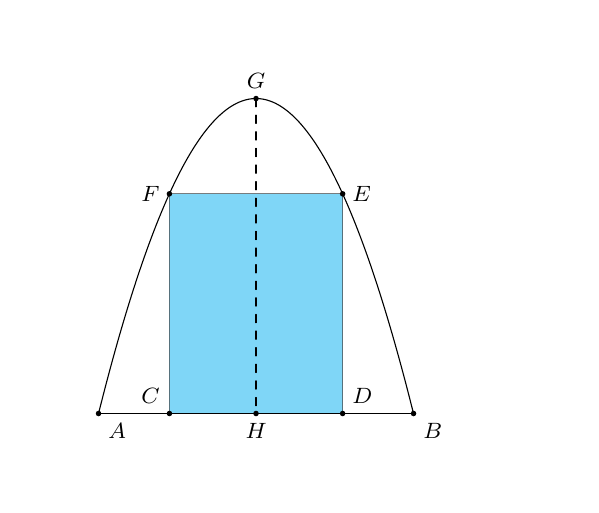
\begin{tikzpicture}[scale=1, font=\footnotesize, line join=round, line cap=round, >=stealth]
			\def\xt{-1} \def\xp{5} \def\yt{5} \def\yd{-1}
			\draw[fill=cyan,opacity=0.5] (0.9,0)--(0.9,2.79)--(3.1,2.79)--(3.1,0)--(0.9,0);
			\clip(\xt+0.1,\yd+0.1) rectangle(\xp+1,\yt-0.1);
			\draw[smooth,samples=300,domain=0:4] plot(\x,{4*(\x)-(\x)^2});
			\fill (0.9,2.79) node[ left]{$F$} circle(1pt);
			\fill (3.1,2.79) node[right]{$E$} circle(1pt);
			\fill (0.9,0) node[above left]{$C$} circle(1pt);
			\fill (3.1,0) node[above right]{$D$} circle(1pt);
			\fill (0,0) node[below right]{$A$} circle(1pt);
			\fill (4,0) node[below right]{$B$} circle(1pt);
			\fill (2,0) node[below]{$H$} circle(1pt);
			\fill (2,4) node[above]{$G$} circle(1pt);
			\draw[dashed] (2,4)--(2,0);
			\draw(0,0)--(4,0);
	\end{tikzpicture}}
	\shortans{$12$}
	\loigiai
	{
		\immini{Gắn hệ trục tọa độ $O x y$ sao cho $A B$ trùng $O x$, $A$ trùng với gốc $O$. Khi đó parabol có đỉnh $G(2 ; 4)$ và đi qua gốc tọa độ.\\
			Giả sử phương trình của parabol có dạng $y=a x^{2}+b x+c$, $(a \neq 0)$.\\
			Vì parabol có đỉnh là $G(2 ; 4)$ và đi qua điểm $O(0 ; 0)$ nên ta có 
			\[\heva{&c=0\\&-\dfrac{b}{2 a}=2\\&a \cdot 2^{2}+b \cdot 2+c=4}\Leftrightarrow\heva{&a=-1 \\&b=4\\&c=0.}\]
		}{
			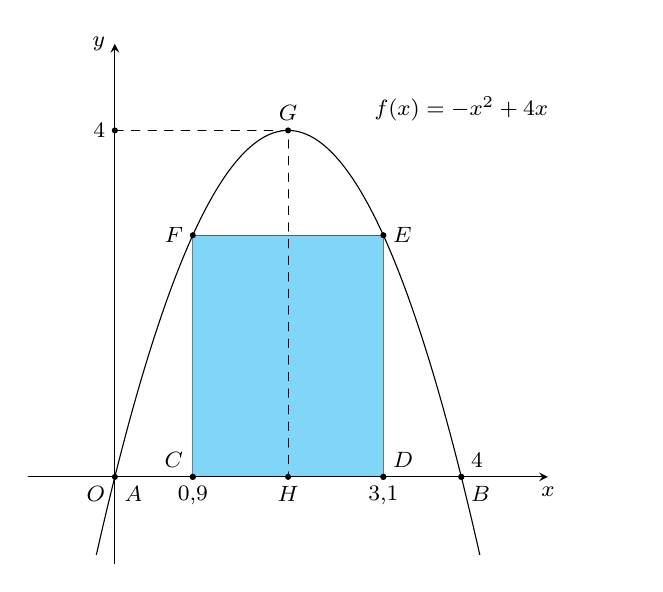
\begin{tikzpicture}[scale=1.1, font=\footnotesize, line join=round, line cap=round, >=stealth]
				\def\xt{-1} \def\xp{5} \def\yt{5} \def\yd{-1}
				\draw[fill=cyan,opacity=0.5] (0.9,0)--(0.9,2.79)--(3.1,2.79)--(3.1,0)--(0.9,0);
				\draw[->](\xt, 0)--(\xp, 0) node[below]{$x$};
				\draw[->](0,\yd)--(0,\yt) node[left]{$y$};
				\node at (0, 0) [below left]{$O$};
				\clip(\xt+0.1,\yd+0.1) rectangle(\xp+1,\yt-0.1);
				\draw[smooth,samples=300] plot(\x,{4*(\x)-(\x)^2});
				\fill (0.9,2.79) node[ left]{$F$} circle(1pt);
				\fill (3.1,2.79) node[right]{$E$} circle(1pt);
				\fill (3.1,0) node[below]{$3{,}1$} circle(1pt);
				\fill (0.9,0) node[below]{$0{,}9$} circle(1pt);
				\fill (0.9,0) node[above left]{$C$} circle(1pt);
				\fill (3.1,0) node[above right]{$D$} circle(1pt);
				\fill (0,0) node[below right]{$A$} circle(1pt);
				\fill (4,0) node[below right]{$B$} circle(1pt);
				\fill (4,0) node[above right]{$4$} circle(1pt);
				\fill (0,4) node[left]{$4$} circle(1pt);
				\fill (2,0) node[below]{$H$} circle(1pt);
				\fill (2,4) node[above]{$G$} circle(1pt);
				\fill (4,4) node[above]{$f(x)=-x^2+4x$};
				\draw[dashed] (0,4)--(2,4)--(2,0);
		\end{tikzpicture}}
		\noindent 		Suy ra phương trình parabol là $y=f(x)=-x^{2}+4 x$.\\
		Diện tích của cả cổng là $S=\displaystyle\int_{0}^{4}\left(-x^{2}+4 x\right) \mathrm{d} x=\left.\left(-\dfrac{x^{3}}{3}+2 x^{2}\right)\right|_{0} ^{4}=\dfrac{32}{3}\mathrm{~m}^{2}$.\\
		Mặt khác chiều cao $C F=D E=f(0{,}9)=2{,}79\mathrm{~m}$; $C D=4-2\cdot0{,}9=2{,}2 \mathrm{~m}$.\\
		Diện tích hai cánh cổng là $S_{\text {CDEF }}=C D \cdot C F=6{,}138 \mathrm{~m}^{2}$.\\
		Diện tích phần để trắng là $S_{1}=S-S_{C D E F}=\dfrac{32}{3}-6{,}138=\dfrac{6\,793}{1\,500} \mathrm{~m}^{2}$.\\
		Vậy tổng số tiền để làm cổng là $6{,}138 \cdot 1\,200\,000+\dfrac{6\,793}{1\,500} \cdot 900\,000=11\,441\,400$ đồng.\\
		Do đó cần ít nhất $12$ triệu đồng.
	}
\end{ex}

% #3424 | Archive/2024/San pham - To Latex Strong - Tex hoa Lop 12 moi - Dot 3 (Chuong 1 + 2 +3 + 4)/Data/Chuong 4/Canh dieu/To 21 - Dot 17 - Chuong 4 - Bai 4 - CD - De 2.tex | mã gốc 2D4V3-2
\begin{ex}%[2D4V3-2]%[Tổ 21 - Đợt 17 - Chương 4 - Bài 4 - Cánh Diều - Đề 2]%[Dương Hồng]
	\immini{Bác Bình muốn làm cửa rào sắt có hình dạng và kích thước như hình vẽ bên, biết đường cong phía trên là một Parabol. Giá $1  \mathrm{m}^{2}$ của rào sắt là $700\,000$ đồng. Hỏi bác Bình phải trả bao nhiêu tiền để làm cái cửa sắt như vậy (nghìn đồng).}{
		\definecolor{apricot}{rgb}{0.98, 0.81, 0.69}
		\begin{tikzpicture}[line join=round, line cap=round,scale=1.2,transform shape]
			
			\tikzset{cong/.pic={
					\def\N{ 
						(-1.8,-1.85)--(-1.8,.25)
						..controls +(30:.4) and +(175:.4) ..(0,.75)--(0,-1.85)--cycle
						(-1.8,0)--(0,0)
						(-1.8,-1.3)--(0,-1.3)
						(-1.2,-1.2) rectangle (-.6,-.15);
						;
					}
					\draw[fill=black!30] (-1.8,-1.8) rectangle (0,-1.3);
					\draw[line width=.4mm,black]\N;
					\draw[fill=black] (0,.75)--(0,-1.85)--(-.1,-1.85)--(-.1,.75)--cycle
					;
					%\fill[ecru!80] \N;
					\draw[pattern=vertical lines,pattern color=black](-1.8,-1.3)rectangle(-1.3,0);
					\draw[pattern=vertical lines,pattern color=black](-.5,-1.3)rectangle(0,0);
					\draw[pattern=vertical lines,pattern color=black](-1.2,-.12)rectangle(-.6,0);
					\draw[pattern=vertical lines,pattern color=black](-1.2,-1.3)rectangle(-.6,-1.2);
					%Cột
					\draw[fill=apricot,apricot,line width=.2mm](-2.3,-1.9)rectangle(-1.82,1.28);
					%\draw[fill=apricot](-3.5,-1.9)rectangle(-2.3,-.5);
					%======================viền cong
					\def\V{ 
						(-1.2,.2)
						..controls +(-110:.4) and +(-35:.4) ..(-1.1,.4)
						..controls +(150:.2) and +(100:.2) ..(-1.3,.1)
						(-.6,.2)
						..controls +(-110:.4) and +(-35:.4) ..(-.5,.4)
						..controls +(150:.2) and +(100:.2) ..(-.7,.1)
						(-.85,.2)
						..controls +(-170:.2) and +(155:.2) ..(-.8,.3)
						..controls +(-20:.2) and +(-55:.24) ..(-1.05,.1)
						(-1.45,.2)
						..controls +(-170:.2) and +(155:.2) ..(-1.4,.3)
						..controls +(-20:.2) and +(-55:.6) ..(-1.8,.25)
						(-.25,.2)
						..controls +(-170:.2) and +(155:.2) ..(-.18,.3)
						..controls +(-20:.2) and +(-55:.24) ..(-.45,.1)
						(-.25,.5)
						..controls +(-170:.2) and +(155:.2) ..(-.18,.7)
						..controls +(-20:.2) and +(-65:.55) ..(-.45,.5)
						(-.55,.52)
						..controls +(-170:.2) and +(155:.2) ..(-.44,.65)
						..controls +(-20:.2) and +(-65:.2) ..(-.75,.5)
						(-.7,.36)
						..controls +(-170:.2) and +(155:.2) ..(-.85,.55)
						..controls +(-20:.2) and +(-55:.25) ..(-1.15,.5)
						;
					}
					\draw[line width=.4mm,black]\V;
					
			}}
			%========================hoa, lá\tikzset{hoa/.pic={
			\tikzset{hoa/.pic={
					\draw (0,0) ..controls +(40:1) and +(170:1) .. (1.6,-2.4)
					(0,0) ..controls +(40:1) and +(170:1) .. (1.6,2.6)
					(0,0) ..controls +(40:1) and +(30:1) .. (-1.4,-2.6)
					(0,0) ..controls +(120:1) and +(80:1) .. (-1.4,2.6);
					\def\H{
						(0,0)
						..controls +(0:2) and +(60:2) .. (0,0)
						..controls +(60:2) and +(120:2) .. (0,0)
						..controls +(120:2) and +(180:2) .. (0,0)
						..controls +(180:2) and +(240:2) .. (0,0)
						..controls +(240:2) and +(300:2) .. (0,0)
						..controls +(300:2) and +(360:2) .. (0,0)
						;}
					\fill[black] \H;
					\draw \H;
					
			}}
			\tikzset{la/.pic={
					\def\L{ 
						(1.6,.95)
						..controls +(30:.5) and +(160:1) ..  (2.4,1.3)
						..controls +(20:0) and +(-160:0.3) ..  (2.9,1.3)
						..controls +(-120:1.4) and +(-120:1) ..  (1.6,.95)
						;}
					\draw \L;
					\fill[black!80] \L;
					%Vẽ gân lá
					\draw (1.35,1.2)
					..controls +(-40:.1) and +(-160:1) ..  (2.5,.9) (2.1,1.15)--(1.7,.84)
					..controls +(-70:.3) and +(170:0) ..  (2,.5)
					(2.2,.82)--(2.5,1.1) (2.3,.78)--(2.5,.8);
			}}
			%==================Mái nhà
			\definecolor{burntsienna}{rgb}{0.91, 0.45, 0.32}                    
			\tikzset{mai/.pic={
					\def\mainha{ 
						(.5,2) 
						foreach \n in {1,2,...,30} { -- ++ (0,0) -- ++ (0,1) -- ++ (1,0) -- ++ (0,-1) } -- cycle
						
						(.25,1) 
						foreach \n in {1,2,...,30} { -- ++ (0,0) -- ++ (0,1) -- ++ (1,0) -- ++ (0,-1) } -- cycle
						
						(0,0) 
						foreach \n in {1,2,...,30} { -- ++ (0,0) -- ++ (0,1) -- ++ (1,0) -- ++ (0,-1) } -- cycle
						;
					}
					\clip (-1.5,-3)--(26.5,-3)--(23.5,3)--(1.5,3)--cycle;
					\draw[fill=burntsienna] \mainha;
					
			}}
			
			
			
			\path (-2.5,1.3)pic[scale=.2]{mai}
			(0,0)pic[scale=1]{cong} (-.9,-.7)pic[scale=.2]{hoa} (-1,-1.7)pic[scale=.2]{la} 
			(-.75,-1.7)pic[rotate=-20,scale=.2]{la} 
			(-.4,-1.8)pic[rotate=140,scale=.2]{la} 
			
			(-1.4,-2)pic[rotate=35,scale=.2]{la} 
			(-.95,-1.9)pic[rotate=125,scale=.3]{la} 
			%-----------
			
			(0,0)pic[scale=1,xscale=-1]{cong}
			(.9,-.7)pic[scale=.2]{hoa} 
			(.89,-1.7)pic[rotate=-5,scale=.2,xscale=-1]{la}
			
			(.72,-1.77)pic[rotate=10,scale=.2,xscale=-1]{la} 
			
			(.3,-1.85)pic[rotate=230,scale=.2,xscale=-1]{la} 
			
			(1.4,-2)pic[rotate=-35,scale=.2,xscale=-1]{la} 
			(.9,-1.8)pic[rotate=225,scale=.3,xscale=-1]{la} 
			;
			
			\draw[dashed] (0,.77)--(2.6,.77);
			\draw[<->,red] (2.6,-1.9)--(2.6,.77);
			\draw[<->,red] (-1.8,-2.1)--(1.8,-2.1);
			\draw[<->,red] (1.9,-1.9)--(1.9,.3);
			\node at (0,-2.3) {\tiny $5$ m};
			\node at (2.9,-.5) {\tiny $2$ m};
			\node at (2.2,-.5) {\tiny $1{,}5$ m};
	\end{tikzpicture}}
	\shortans{$6417$}
	\loigiai{
		Ta chọn hệ trục tọa độ như hình vẽ.
		\begin{center}
			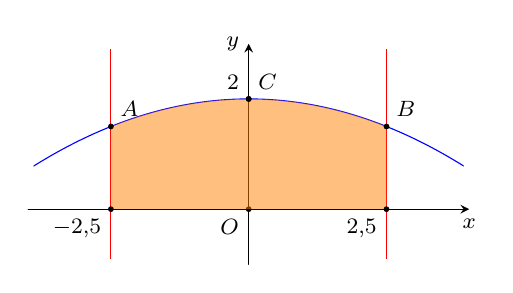
\begin{tikzpicture}[scale=0.7, font=\footnotesize, line join=round, line cap=round, >=stealth]
				\def\xt{-4} \def\xp{4} \def\yt{3} \def\yd{-1}
				\draw[->](\xt, 0)--(\xp, 0) node[below]{$x$};
				\draw[->](0,\yd)--(0,\yt) node[left]{$y$};
				\fill (0,0) node[below left]{$O$} circle(1.5pt);
				\clip(\xt+0.1,\yd+0.1) rectangle(\xp-0.1,\yt-0.1);
				\draw[color=blue, smooth, samples=300] plot(\x,{-0.08*(\x)^2+2});
				\draw[color=red, smooth, samples=300] plot(-2.5,\x);
				\draw[color=red, smooth, samples=300] plot(2.5,\x);
				% Tô màu giữa hai đồ thị
				\fill[fill=orange, opacity=0.5] 
				(-2.5,0) -- plot[samples=300, domain=-2.5:2.5] (\x,{-0.08*(\x)^2+2}) -- (2.5,0) -- cycle;
				\fill (2.5,0) node[below left]{$2{,}5$} circle(1.5pt);
				\fill (-2.5,0) node[below left]{$-2{,}5$} circle(1.5pt);
				\fill (0,2) node[above left]{$2$} circle(1.5pt);
				\fill (0,2) node[above right]{$C$} circle(1.5pt);
				\fill (-2.5,1.5) node[above right]{$A$} circle(1.5pt);
				\fill (2.5,1.5) node[above right]{$B$} circle(1.5pt);
			\end{tikzpicture}
		\end{center}
		Trong đó $A(-2{,}5 ; 1{,}5)$, $B(2{,}5 ; 1{,}5)$, $C(0 ; 2)$.\\
		Giả sử đường cong phía trên là một Parabol có dạng $y=a x^{2}+b x+c$, với $a$; $b$; $c \in \mathbb{Q}$.
		Do Parabol đi qua các điểm $A(-2{,}5 ; 1{,}5)$, $B(2{,}5 ; 1{,}5)$, $C(0 ; 2)$ nên ta có hệ phương trình
		$$
		\heva{&a(-2{,}5)^{2} + b(-2{,}5) + c = 1{,}5\\
			&a(2{,}5 )^{2} + b(2{,}5 ) + c = 1{,}5 \\
			&	c = 2 
		}
		\Leftrightarrow
		\heva{&a=-\dfrac{2}{25} \\
			&b=0\\
			&	c=2.}
		$$
		Khi đó phương trình Parabol là $y=-\dfrac{2}{25} x^{2}+2$.\\
		Diện tích $S$ của cửa rào sắt là diện tích phần hình phẳng giới hạn bởi đồ thị hàm số $y=-\dfrac{2}{25} x^{2}+2$, trục hoành và hai đường thẳng $x=-2{,}5$; $x=2{,}5$.\\
		Ta có $S=\displaystyle\int_{-2{,}5}^{2{,}5}\left(-\dfrac{2}{25} x^{2}+2\right) \mathrm{d} x=\left.\left(-\dfrac{2}{25} \dfrac{x^{3}}{3}+2 x\right)\right|_{-2{,}5} ^{2{,}5}=\dfrac{55}{6}$.\\
		Vậy bác Bình phải trả số tiền để làm cái cửa sắt là
		$$S \times 700\,000=\dfrac{55}{6} \times 700\,000 \approx 6\,416 \,667 \text{( đồng).}$$ 
		Hay $6\,417$ nghìn đồng.
	}
\end{ex}

% #3435 | Archive/2024/San pham - To Latex Strong - Tex hoa Lop 12 moi - Dot 3 (Chuong 1 + 2 +3 + 4)/Data/Chuong 4/Canh dieu/To 21 - Dot 17 - Chuong 4 - Bai 4 - CD - De 1.tex | mã gốc 2D4V3-3
\begin{ex}%[2D4V3-3]
	\immini{
	Từ hình chữ nhật $ABCD$ có chiều dài $AB=10$ cm và chiều rộng $BC=5$ cm. Người ta cắt bỏ miền $(R)$ được giới hạn bởi cạnh $CD$ của hình chữ nhật và hai nửa đường parabol có chung đỉnh là trung điểm của cạnh $AB$, chúng lần lượt đi qua hai đầu mút $C$, $D$ của hình chữ nhật đó (phần tô đậm như hình vẽ). 
	}
	{
	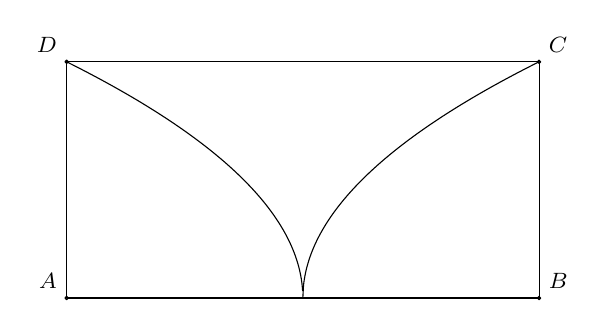
\begin{tikzpicture}[scale=.6, font=\footnotesize, line join=round, line cap=round, >=stealth]
		\tikzset{label style/.style={font=\footnotesize}}
		%Nhập giới hạn đồ thị và hàm số cần vẽ
		%\pgfmathsetmacro{\so}{sqrt{5}}
		\def \hamso{sin((2*(\x))*180/pi)}
		%\def \tiemcanxien{\x+1}
		%Tự động
	%	\draw[->] (-5.5,0)--(6,0) node[below left] {$x$};
	%	\draw[->] (0,-0.5)--(0,6) node[below left] {$y$};
	%	\draw[fill=black] (0,0) circle(1pt) node [below right] {$O$};
		%Vẽ các điểm trên 2 hệ trục
		\draw
		(-5,0) coordinate (A) circle(1pt) node[above left]{$A$} %node[below]{$-5$}
		(5,0) coordinate (B) circle(1pt) node[above right]{$B$} %node[below]{$5$}
		(-5,5) coordinate (D) circle(1pt) node[above left]{$D$}
		(5,5) coordinate (C) circle(1pt) node[above right]{$C$}
		%(0,5) circle(1pt) node[above right]{$5$}
		;
		\draw
		(A)--(B)--(C)--(D)--cycle;
		%Tự động
		\begin{scope}
			\draw[samples=350,domain=0:5,smooth,variable=\x] plot (\x,{sqrt(5*\x)});
			\draw[samples=350,domain=-5:0,smooth,variable=\x] plot (\x,{sqrt{-5*(\x)}});
		\end{scope}
	\end{tikzpicture}
	}
\noindent Phần còn lại cho quay quanh trục $AB$ để tạo nên một đồ vật làm trang trí, thể tích của vật trang trí đó bằng bao nhiêu? (làm tròn đến hàng đơn vị).
	\shortans[]{393}
	\loigiai{
	\begin{center}
		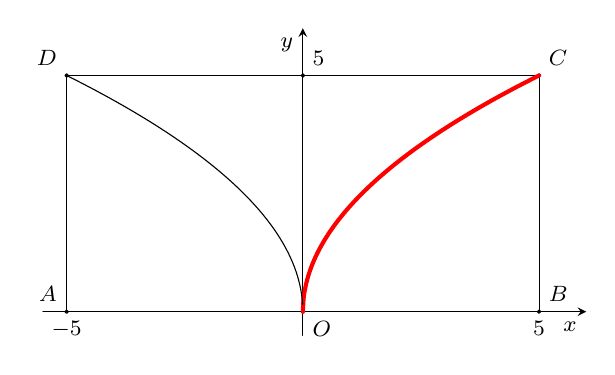
\begin{tikzpicture}[scale=.6, font=\footnotesize, line join=round, line cap=round, >=stealth]
			\tikzset{label style/.style={font=\footnotesize}}
			%Nhập giới hạn đồ thị và hàm số cần vẽ
			%\pgfmathsetmacro{\so}{sqrt{5}}
			\def \hamso{sin((2*(\x))*180/pi)}
			%\def \tiemcanxien{\x+1}
			%Tự động
			\draw[->] (-5.5,0)--(6,0) node[below left] {$x$};
			\draw[->] (0,-0.5)--(0,6) node[below left] {$y$};
			\draw[fill=black] (0,0) circle(1pt) node [below right] {$O$};
			%Vẽ các điểm trên 2 hệ trục
			\draw
			(-5,0) coordinate (A) circle(1pt) node[above left]{$A$} node[below]{$-5$}
			(5,0) coordinate (B) circle(1pt) node[above right]{$B$} node[below]{$5$}
			(-5,5) coordinate (D) circle(1pt) node[above left]{$D$}
			(5,5) coordinate (C) circle(1pt) node[above right]{$C$}
			(0,5) circle(1pt) node[above right]{$5$}
			;
			\draw
			(A)--(B)--(C)--(D)--cycle;
			%Tự động
			\begin{scope}
				\draw[line width=1.5,color=red,samples=350,domain=0:5,smooth,variable=\x] plot (\x,{sqrt(5*\x)});
				\draw[samples=350,domain=-5:0,smooth,variable=\x] plot (\x,{sqrt{-5*(\x)}});
			\end{scope}
		\end{tikzpicture}
	\end{center}
	Khi quay hình chữ nhật $ABCD$ quanh trục $AB$ ta được khối trụ có bán kính đáy $r=BC=5$ cm, chiều cao $h=AB=10$ cm.\\
	Do đó thể tích khối trụ này có thể tích $V_1=\pi \cdot 5^2\cdot 10=250\pi$ (cm$^3$).\\
	Mặt khác, chọn hệ trục tọa độ như hình vẽ thì $C(5;5)$ và parabol bên phải trục $Ox$ có dạng $(P_1)\colon y^2=2px$.\\
	Ta có $C\in (P_1)\Leftrightarrow p=\dfrac{5}{2}
	\Rightarrow (P_1)\colon y^2=5x$ hay $y=\sqrt{5x}$.\\
	Khi đó miền $(R)$ khi quay quanh trục $Ox$ có thể tích $V_2=2\pi \displaystyle \int\limits_0^5 \left[ {5^2}-5x \right]\,\mathrm{\,d}x=2\pi \left. \left( 25x-\dfrac{5}{2}{x^2} \right) \right|_0^5=125\pi $.\\
	Vậy thể tích phần còn lại là $V=V_1-V_2=125\pi$ (cm$^3$).\\
}
	\end{ex}

% #3439 | Archive/2024/San pham - To Latex Strong - Tex hoa Lop 12 moi - Dot 3 (Chuong 1 + 2 +3 + 4)/Data/Chuong 4/Canh dieu/To 19 - Dot 17 - Chuong 4 - Bai 2 - CD - De 1.tex | mã gốc 2D4V1-6
\begin{ex}%[2D4V1-6]
Một vận động viên điền kinh chạy với gia tốc $a(t)=-\dfrac{1}{24} t^{3}+\dfrac{5}{16} t^{2}\left(\mathrm{~m} / \mathrm{s}^{2}\right)$, trong đó $t$ là khoảng thời gian tính từ lúc xuất phát.
\choiceTF
{\True Phương trình vận tốc của vận động viên điền kinh là $v(t)=-\dfrac{1}{96} t^{4}+\dfrac{5}{48} t^{3}(\mathrm{~m} / s)$}
{\True  Phương trình quãng đường của vận động viên điền kinh là $S(t)=-\dfrac{1}{480} t^{5}+\dfrac{5}{192} t^{4}(m)$}
{Quãng đường vận động viên chạy được trong $5$ giây đầu tiên là $9{,}57$ (m)}
{\True Quãng đường vận động viên chạy được cho đến lúc dừng chuyển động là $52{,}08$(m) (Làm tròn đến chữ số thập phân thứ hai)}
\loigiai{
\begin{itemchoice}
	\itemch  Đúng.\\
	Vì Vận tốc $v(t)$ chính là nguyên hàm của gia tốc $a(t)$ nên ta có
	$$v(t)=\int a(t)  \mathrm{d}t=\int\left(-\dfrac{1}{24} t^{3}+\dfrac{5}{16} t^{2}\right)  \mathrm{d}t=-\dfrac{1}{96} t^{4}+\dfrac{5}{48} t^{3}+C$$
	Tại thời điểm ban đầu $(t=0)$ thì vận động viên ở vị trí xuất phát nên $$v(0)=-\dfrac{1}{96} 0^{4}+\dfrac{5}{48} 0^{3}+C=0 \Leftrightarrow C=0$$ 
	Nên $v(t)=-\dfrac{1}{96} t^{4}+\dfrac{5}{48} t^{3}$ (m/s).
	\itemch Đúng.\\
	Vì quãng đường $s(t)$ chính là nguyên hàm của vận tốc $v(t)$ nên ta có
	$$s(t)=\int v(t) \mathrm{d}t=\int-\dfrac{1}{96} t^{4}+\dfrac{5}{48} t^{3}=-\dfrac{1}{480} t^{5}+\dfrac{5}{192} t^{4}+\mathrm{C}$$
	Tại thời điêm ban đầu $(t=0)$ thì vận động viên ở vị trí xuất phát nên
	$$S(0)=-\dfrac{1}{480} 0^{5}+\dfrac{5}{192} 0^{4}+C=0 \Leftrightarrow C=0$$ 
	Nên $S(t)=-\dfrac{1}{480} t^{5}+\dfrac{5}{192} t^{4}$ (m)
	\itemch Sai.\\
	Vì Tại thời điểm ban đầu $(t=10)$ thì vận động viên chạy được
	$$S(10)=-\dfrac{1}{480} \cdot 5^{5}+\dfrac{5}{192} \cdot 5^{4} \approx 9{,}77 \text{ (m)}$$
	\itemch Đúng.\\
	Vì vận tốc $v(t)=-\dfrac{1}{96} t^{4}+\dfrac{5}{48} t^{3}(\mathrm{~m} / s)$\\
	 Khi vận động viên dừng chuyển động thì $v(t)=0 \Leftrightarrow-\dfrac{1}{96} t^{4}+\dfrac{5}{48} t^{3}=0 \Leftrightarrow\left[\begin{array}{l}t=0 \\ t=10\end{array}\right.$\\
	$S(10)=-\dfrac{1}{480} \cdot 10^{5}+\dfrac{5}{192} \cdot 10^{4} \approx 52{,}08$ (m).
\end{itemchoice}
}
\end{ex}

% #3445 | Archive/2024/San pham - To Latex Strong - Tex hoa Lop 12 moi - Dot 3 (Chuong 1 + 2 +3 + 4)/Data/Chuong 4/Canh dieu/To 19 - Dot 17 - Chuong 4 - Bai 2 - CD - De 1.tex | mã gốc 2D4V1-6
\begin{ex}%%[2D4V1-6]
 \immini{Một vật chuyển động trong $4$ giờ với vận tốc $v$ (km / h) phụ thuộc vào thời gian $t$ (h) có đồ thị vận tốc là một đường parabol có đỉnh $I(3 ; 10)$ và trục đối xứng vuông góc với trục hoành như hình vẽ. Tính quãng đường vật di chuyển được trong nửa thời gian sau của chuyển động đó (kết quả làm tròn đến hàng phần chục và tính theo đơn vị km )}
 {
 	\begin{tikzpicture}[scale=0.4,>=stealth, font=\footnotesize, line join=round, line cap=round]
 	\def\xmin{-3} \def\xmax{6}
 	\def\ymin{-1} \def\ymax{11}
 	\draw[->] (\xmin,0)--(\xmax,0) node [below]{$t$};
 	\draw[->] (0,\ymin)--(0,\ymax) node [left]{$v$};
 	\fill (0,0) circle (1pt) node[shift={(-135:2.5mm)}]{$O$};
 	\clip (\xmin+0.1,\ymin+0.1) rectangle (\xmax-0.1,\ymax-0.1);
 	\draw[smooth,red,samples=300,domain=(0:4)] plot(\x,{-(\x)^2+6*(\x)+1});	
 	\foreach \x in {\xmin,...,\xmax}
 	\draw (\x,-0.05)--(\x,0.05);
 	\foreach \y in {\ymin,...,\ymax}
 	\draw (-0.05,\y)--(0.05,\y);	
 	\node at (3,0)[below]{$3$};
 	\node at (0,1)[left]{$1$};
 	\node at (0,10)[left]{$10$};
 	\draw[dashed] (0,10)--(3,10)--(3,0);
 	%\node at (-1,1)[shift={(70:2mm)}]{$ I $};
 	%\draw[dashed]
 	%(-1,0)node[below]{$ -1 $}|-(0,1)node[right]{$1$}	
 %	;	
 \end{tikzpicture}
 }
\shortans{$19{,}3$}

\loigiai{
Dựa vào đồ thị ta tìm được vận tốc $v(t)=-t^{2}+6 t+1, t \in[0 ; 4]$.\\
Quãng đường $s(t)$ vật di chuyển được trong thời gian $4$h là một nguyên hàm của $v(t)$, với $t \in[0 ; 4]$\\
Ta có $s(t)=\displaystyle\int\left(-t^{2}+6t+1\right) \mathrm{d}t=-\dfrac{t^{3}}{3}+3 t^{2}+t+C$.\\
Quãng đường vật di chuyển được trong $2$h đầu là $s(2)=\dfrac{34}{3}+C$ (km).\\
Quãng đường vật di chuyển được trong $4$h là $s(4)=\dfrac{92}{3}+C$ (km).\\
Quãng đường vật di chuyển được trong nửa thời gian sau của chuyển động là
$$s(4)-s(2)=\dfrac{58}{3} \text{~(km)} \approx 19{,}3\text{~(km)}.$$}

\end{ex}

% #3449 | Archive/2024/San pham - To Latex Strong - Tex hoa Lop 12 moi - Dot 3 (Chuong 1 + 2 +3 + 4)/Data/Chuong 4/Canh dieu/To 19 - Dot 17 - Chuong 4 - Bai 2 - CD - De 2.tex | mã gốc 2D4V4-6
\begin{ex}%[2D4V4-6]%[Tổ 1 - Đợt 17 - Chương 4 - Bài 2 - CD - Đề 2]%[Phùng Minh Phúc]
	\immini{Một em bé ném một viên bi lăn trên sàn nhà. Viên bi chuyển động chậm dần đều với tốc độ $v\left( t \right)=9-2t\left( \text{m}/\text{s} \right)$, trong đó $t$ là thời gian tính bằng giây kể từ lúc thả bi. Gọi $s\left( t \right)$ là quãng đường viên bi lăn được trong $t$ (giây) kể từ lúc ném bi.
		}{
		\tikzset{every picture/.style={line width=0.75pt}} %set default line width to 0.75pt        
		
		
\begin{tikzpicture}[x=0.75pt,y=0.75pt,yscale=-0.5,xscale=0.5]
			%uncomment if require: \path (0,300); %set diagram left start at 0, and has height of 300
			
			%Shape: Rectangle [id:dp01193065481495248] 
			\draw  [color={rgb, 255:red, 65; green, 117; blue, 5 }  ,draw opacity=1 ][fill={rgb, 255:red, 110; green, 185; blue, 29 }  ,fill opacity=1 ] (101,98) -- (581,98) -- (581,117) -- (101,117) -- cycle ;
			%Shape: Rectangle [id:dp32385753291806374] 
			\draw  [color={rgb, 255:red, 139; green, 87; blue, 42 }  ,draw opacity=1 ][fill={rgb, 255:red, 139; green, 87; blue, 42 }  ,fill opacity=1 ] (101,117) -- (581,117) -- (581,191) -- (101,191) -- cycle ;
			%Shape: Ellipse [id:dp7690339144350697] 
			\draw  [fill={rgb, 255:red, 108; green, 14; blue, 192 }  ,fill opacity=1 ] (110.25,63.75) .. controls (110.25,45.11) and (125.92,30) .. (145.25,30) .. controls (164.58,30) and (180.25,45.11) .. (180.25,63.75) .. controls (180.25,82.39) and (164.58,97.5) .. (145.25,97.5) .. controls (125.92,97.5) and (110.25,82.39) .. (110.25,63.75) -- cycle ;			
		\end{tikzpicture}
}
\choiceTF[1]
{\True $s\left( t \right)=9t-{{t}^{2}}$}
{Vật chuyển động với gia tốc là $a(t)=2\left( \text{m}/{{\text{s}}^{2}} \right)$}
{Quãng đường viên bi lăn được trong $3$ giây đầu tiên là $18$ m}
{Quãng đường viên bi lăn được từ lúc em bé ném bi đến khi dừng hẳn là $36$ m}
	\loigiai{
		\begin{itemchoice}
			\itemch \textbf{Đúng}.\\
			Ta có $s\left( t \right)=\displaystyle\int\limits v\left( t \right)\text{d}t=\displaystyle\int\limits \left(9-2t \right)\text{d}t=9t-{{t}^{2}}+C$.\\
			Do $s\left( 0 \right)=0$ nên $C=0$.\\
			Suy ra $s\left( t \right)=9t-{{t}^{2}}$.
			\itemch \textbf{Sai}.\\
			Ta có $a\left( t \right)={v}'\left( t \right)={(9-2t)}=-2\,\left( \text{m}/{{\text{s}}^{2}} \right)$.
			\itemch \textbf{Sai}.\\
			Ta có $s\left( t \right)=9t-{{t}^{2}}$.\\
			Quãng đường viên bi lăn được trong $3$ giây đầu tiên là $s\left( 3 \right)-s\left( 0 \right)=18$ m.
			\itemch \textbf{Sai}.\\
			Thời điểm viên bi dừng hẳn là $9-2t=0\Leftrightarrow t=\dfrac{9}{2}$.\\
			Quãng đường viên bi lăn được từ lúc em bé thả bi đến khi dừng hẳn là $s\left( \dfrac{9}{2} \right)-s\left( 0 \right)=20{,}25\,\text{m}$.
		\end{itemchoice}
	}
	\end{ex}

% #3455 | Archive/2024/San pham - To Latex Strong - Tex hoa Lop 12 moi - Dot 3 (Chuong 1 + 2 +3 + 4)/Data/Chuong 4/Canh dieu/To 19 - Dot 17 - Chuong 4 - Bai 2 - CD - De 2.tex | mã gốc 2D4V4-6
\begin{ex}%[2D4V4-6]%[Tổ 1 - Đợt 17 - Chương 4 - Bài 2 - CD - Đề 2]%[Phùng Minh Phúc]
	Tại một khu di tích vào ngày lễ hội, người ta tính được tốc độ thay đổi lượng khách tham quan được biểu diễn bằng hàm số $\text{{Q}'}\left( t \right)=4{{t}^{3}}-72{{t}^{2}}+288t$, trong đó $t$ tính bằng giờ $\left( 0\le t\le 13 \right),Q'\left( t \right)$ tính bằng khách/giờ. Sau $2$ giờ đã có 500 người có mặt.
	\begin{enumerate}[a)]
		\item Xác định hàm số $Q\left( t \right)$ biểu diễn lượng khách tham quan di tích.
		\item Xác định thời điểm mà lượng khách tham quan lớn nhất.
		\item Tìm thời điểm mà tốc độ thay đổi lượng khách tham quan là lớn nhất?
	\end{enumerate}
	\shortans[oly]{}
	\loigiai{
			\begin{enumerate}[a)]
			\item Ta có $Q\left( t \right)=\displaystyle\int\limits Q'\left( t \right)\text{d}t=\displaystyle\int\limits \left( 4{{t}^{3}}-72{{t}^{2}}+288t \right)\text{d}t={{t}^{4}}-24{{t}^{3}}+144{{t}^{2}}+C$.\\
			Mà sau $2$ giờ đã có $500$ người nên ta có $Q\left( 2 \right)=500$ suy ra $C=100$.\\
			Vậy $Q\left( t \right)={{t}^{4}}-24{{t}^{3}}+144{{t}^{2}}+100$.
			\item Ta tìm giá trị lớn nhất của hàm số $Q\left( t \right)$ trên đoạn $\left[ 0;13 \right]$.\\
			Ta có ${Q}'\left( t \right)=0$ khi $t=0,t=6$ và $t=12$.\\
			Mà $Q\left( 0 \right)=100,Q\left( 6 \right)=1\,396,Q\left( 12 \right)=100,Q\left( 13 \right)=269$.\\
			Nên lượng khách tham quan lớn nhất là sau $6$ giờ, có $1\,396$ người.
			\item Khảo sát hàm số ${Q}'\left( t \right)=4{{t}^{3}}-72{{t}^{2}}+288t$ trên đoạn $\left[ 0;13 \right]$.\\
			Ta có ${Q}''\left( t \right)=12{{t}^{2}}-144t+288$.\\
			${Q}''\left( t \right)=0\Leftrightarrow 12{{t}^{2}}-144t+288=0\Leftrightarrow t=6-2\sqrt{3}$ hoặc $t=6+2\sqrt{3}$.\\
			Bảng biến thiên của hàm số ${Q}'\left( t \right)$ như sau:
			\begin{center}
				
\begin{tikzpicture}
					\tkzTabInit[lgt=2,espcl=4]
					{$t$/0.7,$Q''(t)$/0.7,$Q'(t)$/3}
					{$0$,$6-2\sqrt{3}$,$6+2\sqrt{3}$,$13$}
					\tkzTabLine{,+,0,-,0,+}
					\tkzTabVar{-/$0$,+/$Q^{\prime}(6-2\sqrt{3})$,-/$Q^{\prime}(6+2\sqrt{3})$,+/$364$}
				\end{tikzpicture}
			\end{center}
			Với ${Q}'\left( 6-2\sqrt{3} \right)\approx 332,6$ và ${Q}'\left( 6+2\sqrt{3} \right)\approx -332{,}6$.\\
			Vậy tốc độ thay đổi lượng khách tham quan lớn nhất tại thời điểm $t=13$.
		\end{enumerate}
	}
\end{ex}

% #3789 | Archive/SP_KhoLatex/SP_Đề Theo Bài-Khối 12/2-B13-De1.tex | mã gốc 2D4V3-2
\begin{ex}%[2D4V3-2]
	\immini{
		Một chiếc cổng có hình dạng là một parabol $(P)$ có kích thước như hình vẽ, biết chiều cao cổng bằng $4$m, $AB=4$m. Người ta thiết kế cửa đi là một hình chữ nhật $CDEF$ (với $C,F\in AB;\ D,E\in (P)$), phần còn lại (\textit{phần tô đậm}) dùng để trang trí. Biết chi phí để trang trí phần tô đậm là $1\,000\,000$ đồng/m$^2$. Gắn hệ trục tọa độ $Oxy$ như hình bên.
	}{
		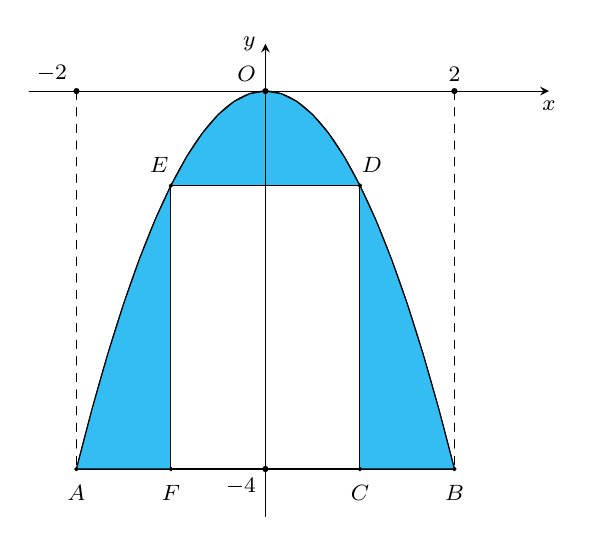
\begin{tikzpicture}[>=stealth,line join=round,line cap=round,font=\footnotesize,scale=.6]
			\path 
			(2,-2)coordinate(D)
			(-2,-2)coordinate(E)
			(2,-8)coordinate(C)
			(-2,-8)coordinate(F)
			(-4,-8)coordinate(A)
			(4,-8)coordinate(B)
			;
			\draw[smooth,samples=100,domain=-4:4] plot(\x,{-0.5*(\x)^2});
			\draw (C)--(D)--(E)--(F) (A)--(B);
			\draw[fill=cyan!80] (A) plot[domain=-4:4](\x,{-0.5*(\x)^2}) (B)--(A);
			\draw[fill=white] (C)--(D)--(E)--(F)--(C);
			\draw[->] (-5,0)--(6,0) node[below] {$x$};
			\draw[->] (0,-9)--(0,1) node[left] {$y$};
			\draw[fill=black] (0,0) node[above left=-0.1] {$O$} circle (1.5pt);
			\draw[fill=black] (0,-8) node[below left=-0.1] {$-4$} circle (1.5pt);
			\draw[fill=black] (-4,0) node[above left=-0.1] {$-2$} circle (1.5pt);
			\draw[fill=black] (4,0) node[above] {$2$} circle (1.5pt);
			\draw[dashed] (-4,0)--(-4,-8) (4,0)--(4,-8);
			\foreach \p/\g in {A/-90,F/-90,C/-90,B/-90,E/120,D/60}
			\draw[fill=black] (\p) circle (1pt) node[shift=(\g:3mm)] {$\p$};
		\end{tikzpicture}
	}
	\choiceTF
	{\True Parabol đi qua điểm $A(-2;4)$}
	{Phương trình của chiếc cổng parabol là $y=x^2$}
	{\True Diện tích cổng parabol (tính luôn cả cửa đi) là $\dfrac{32}{3}$}
	{Số tiền dùng để trang trí nhỏ nhất là $4\,000\,000$ đồng}
	\loigiai{
		\begin{itemchoice}
			\itemch Parabol đi qua điểm $A(-2;4)$
			\itemch Parabol có phương trình $y=ax^2+bx+c$.\\
			Parabol đi qua $3$ điểm $A(-2;-4)$, $O(0;0)$ và $B(2;-4)$ nên ta có
			$$\heva{&4a-2b+c=-4\\&4a+2b+c=-4\\&c=0}\Leftrightarrow\heva{&a=-1\\&b=0\\&c=0.}$$
			Khi đó, parabol có phương trình là $y=x^2$.
			\itemch Diện tích của hình phẳng giới hạn bởi parabol $(P)$ và đường thẳng $y=-4$ bằng
			$$S_1=\displaystyle\int\limits_{-2}^{2}\left|-x^2+4\right|\mathrm{d}x=\dfrac{32}{3}.$$
			\itemch Gọi $D\left(t,-t^2\right)\in(P)$ với $0<t<2$. Diện tích của hình chữ nhật $CDEF$ là\\
			\[S_2=2t\cdot \left(-t^2+4\right)=-2t^3+8t.\]
			Diện tích phần trang trí
			\[S=S_1-S_2=2t^3-8t+\dfrac{32}{3}.\]
			Để số tiền dùng để trang trí nhỏ nhất thì diện tích phần trang trí nhỏ nhất.\\
			Xét hàm $f(t)=2t^3-8t+\dfrac{32}{3}$ trên $(0;2)$. Ta có
			\[f'(t)=6t^2-8=0\Rightarrow t= \dfrac{2}{\sqrt{3}}.\]
				Bảng biến thiên
				\begin{center}
					
\begin{tikzpicture}[>=stealth]
						\tkzTabInit[lgt=1.5,espcl=2.5]
						{$t$ /1.2, $f'(t)$ /1, $f(t)$ /2}
						{$0$, $\dfrac{2}{\sqrt{3}}$, $2$}
						\tkzTabLine{,-,0,+,}
						\tkzTabVar{+/ $\dfrac{32}{3}$, -/ $f_{\text{CT}}$, +/ $\dfrac{32}{3}$}
					\end{tikzpicture}
				\end{center}
			Do đó, $\min\limits_{(0;2)}f(t)=f\left(\dfrac{2}{\sqrt{3}}\right)=\dfrac{96-32\sqrt{3}}{9}\approx 4{,}5083$.\\
				Vậy số tiền dùng để trang trí nhỏ nhất gần bằng	$4{,}508\cdot 1\,000\,000=4\,508\,000\ \text{đồng}.$
		\end{itemchoice}
	}
\end{ex}

% #3790 | Archive/SP_KhoLatex/SP_Đề Theo Bài-Khối 12/2-B13-De1.tex | mã gốc 2D4V3-5
\begin{ex}%[2D4V3-5]
	Một thùng rượu vang có dạng khối tròn xoay với bán kính mặt đáy và mặt ở trên là $33$ cm, bán kính mặt cắt ở chính giữa thùng là $43$ cm. Chiều cao của thùng rượu là $112$ cm, bao gồm phần thân thùng rượu, hai đế đỡ thùng rượu (mỗi đế cao $3$ cm) và thùng rượu được ghép từ các thanh gỗ sồi với độ dày mỗi thanh gỗ là $3$ cm (Hình 1a). Hình 1b mô phỏng phần bên trong thùng rượu có dạng một khối tròn xoay tạo thành khi quay một phần của parabol $(P)\colon y=ax^2+bx+c$ quanh trục hoành (mỗi đơn vị ứng với $10$ cm).
	\begin{center}
		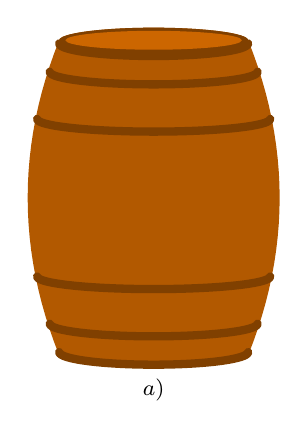
\begin{tikzpicture}[scale=0.4, font=\footnotesize, line join=round, line cap=round,>=stealth]
			\begin{scope}[rotate=90]
				\fill[orange!70!black, draw=none] (-5,-3)arc (-90:-270: 0.4 and 3)--(-5,3)--plot[domain=-5:5](\x,{-1/25*(\x)^2+4})--(5,3)arc (90:-90: 0.4 and 3)--(5,-3)--plot[domain=5:-5](\x,{1/25*(\x)^2-4})--cycle;
				\fill[orange!50!black,draw=none] (5,0) ellipse (0.4 and 3);
				\fill[orange!80!black,draw=none] (5,0) ellipse (0.3 and 2.8);
				\draw[color=orange!50!black,line width=3pt] (4.9,3) arc (90:270: 0.4 and 3);
				\draw[color=orange!50!black,line width=3pt] (4,3.3) arc (90:270: 0.4 and 3.3);
				\draw[color=orange!50!black,line width=3pt] (2.5,3.7) arc (90:270: 0.4 and 3.7);
				\draw[color=orange!50!black,line width=3pt] (-2.5,3.7) arc (90:270: 0.4 and 3.7);
				\draw[color=orange!50!black,line width=3pt] (-4,3.3) arc (90:270: 0.4 and 3.3);
				\draw[color=orange!50!black,line width=3pt] (-4.9,3) arc (90:270: 0.4 and 3);
			\end{scope}
			\node[below] at (current bounding box.south){$a)$};
		\end{tikzpicture}
		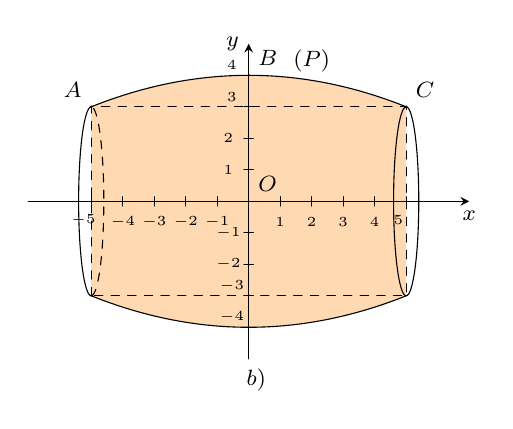
\begin{tikzpicture}[scale=0.4, font=\footnotesize, line join=round, line cap=round,>=stealth]
			\fill[color=orange!30, draw=none] (-5,-3)--(-5,3)--plot[domain=-5:5](\x,{-1/25*(\x)^2+4})--(5,3)--(5,-3)--plot[domain=5:-5](\x,{1/25*(\x)^2-4})--cycle;
			\draw[->] (-7,0) --(7,0) node[below]{$x$};
			\draw[->] (0,-5) --(0,5) node[left]{$y$};
			\draw (0,0) node[above right]{$O$};
			\draw[smooth,samples=200,domain=-5:5] plot(\x,{-1/25*(\x)^2+4});
			\draw[smooth,samples=200,domain=-5:5] plot(\x,{1/25*(\x)^2-4});
			\draw (5,0) ellipse (0.4 and 3);
			\draw (-5,3) arc (90:270: 0.4 and 3);
			\draw[dashed] (-5,-3) arc (-90:90: 0.4 and 3);
			\draw[dashed] (-5,-3)--(-5,3)--(5,3)--(5,-3)--cycle;
			\fill[color=black] 
			(-5,3) node[above left] {$A$} circle (1.25pt)
			(0,4) node[above right] {$B$} circle (1.25pt)
			(5,3) node[above right] {$C$} circle (1.25pt)
			(2,3.8) node[above] {$(P)$}
			;
			\foreach \x in {-2,-1,1,2}
			\draw (0.15,\x)--(-0.15,\x) node[shift={(180:2mm)},font=\tiny]{$\x$};
			\foreach \x in {-4,-3,3,4}
			\draw (0.15,\x)--(-0.15,\x) node[shift={(140:2mm)},font=\tiny]{$\x$};
			\foreach \x in {-4,-3,-2,-1,1,2,3,4}
			\draw (\x,0.15)--(\x,-0.15) node[shift={(-90:2mm)},font=\tiny]{$\x$};
			\foreach \x in {-5,5}
			\draw (\x,0.15)--(\x,-0.15) node[shift={(-120:2mm)},font=\tiny]{$\x$};
			\node[below] at (current bounding box.south){$b)$};
		\end{tikzpicture}\\
		\textit{Hình 1}
	\end{center}
\choiceTF
{\True Phần bên trong thùng rượu có chiều cao là $100$ cm}
{Hệ số $b=0$ và $c=20$}
{\True Parabol $(P)$ có phương trình $y=-\dfrac{1}{250}x^2+40$}
{\True Thùng rượu đó chứa được tối đa $425{,}16$ lít rượu (làm tròn kết quả đến hàng phần trăm)}
	\loigiai{
		\begin{itemchoice}
			\itemch Chiều cao bên trong của thùng rượu là $112-3\cdot 4=100$ (cm).
			\itemch  Parabol $(P)$ có đỉnh $B(0;40)$ nên $b=0$, $c=40$.
			\itemch Mặt khác $(P)$ đi qua $C(50;30)$ nên suy ra
			$$ 30=a\cdot 50^2+0\cdot 50+40\Leftrightarrow 2500 a=-10\Leftrightarrow a=-\dfrac{1}{250}. $$
			Vậy $a=-\dfrac{1}{250}$, $b=0$, $c=40$.
			\itemch Thể tích thùng rượu (tính bằng đơn vị $\mathrm{cm}^3$) bằng thể tích khối tròn xoay tạo thành khi quay quanh $Ox$ hình phẳng giới hạn bởi $(P)$, trục $Ox$ và hai đường thẳng $x=-50$, $x=50$. Vậy số lít rượu tối đa mà thùng rượu chứa được là
			$$ V=\dfrac{1}{1000}\cdot \pi \int\limits_{-50}^{50} \left(-\dfrac{1}{250}x^2+40\right)^2\,\mathrm{d}x=\dfrac{406\pi}{3}\approx 425{,}16\quad (\text{lít}). $$
		\end{itemchoice}
	}
\end{ex}

% #3795 | Archive/SP_KhoLatex/SP_Đề Theo Bài-Khối 12/2-B13-De1.tex | mã gốc 2D4V3-2
\begin{ex}%[2D4V3-2]
	\immini
	{
		Một gia đình muốn làm cánh cổng (như hình vẽ). Phần phía trên cổng có hình dạng là một parabol với $IH=2{,}5$ m, phần phía dưới là một hình chữ nhật kích thước cạnh là $AD=4$ m, $A B=6$ m. Giả sử giá để làm phần cổng được tô màu là $1\,000\,000 \text{~đồng} / \mathrm{m}^2$ và giá để làm phần cổng phía trên là $1\,200\,000 \text{~đồng} / \mathrm{m}^2$. Số tiền tổng cộng gia đình cần trả là bao nhiêu triệu đồng?
	}
	{
		\begin{tikzpicture}[scale=0.7, font=\footnotesize, line join=round, line cap=round, >=stealth]
			\draw (-3,-2.5) parabola bend (0,0) (3,-2.5);
			\fill (0,0)coordinate (I)  circle (1pt) node[above]{$I$};
			\fill (0,-2.5)coordinate (H)  circle (1pt) node[above right]{$H$};
			\fill (-3,-2.5)coordinate (A)  circle (1pt) node[left]{$A$};
			\fill (3,-2.5)coordinate (B)  circle (1pt) node[right]{$B$};
			\fill (-3,-6.5)coordinate (D)  circle (1pt) node[left]{$D$};
			\fill (3,-6.5)coordinate (C)  circle (1pt) node[right]{$C$};
			\draw (I)--(H) node[midway, right]{$2{,}5$ m};
			\draw (A)--(D) node[midway, left]{$4$ m};
			\draw (D)--(C) node[midway, below]{$6$ m};
			\draw[pattern = north east lines] (-3,-2.5) rectangle (3,-6.5);
		\end{tikzpicture}
	}
\shortans{$36$}
	\loigiai{
		\begin{center}
			\begin{tikzpicture}[scale=0.8, font=\footnotesize, line join=round, line cap=round, >=stealth]
				\draw (-3,-2.5) parabola bend (0,0) (3,-2.5);
				\draw (-11,-2.5) parabola bend (-8,0) (-5,-2.5);
				\draw[->] (-8,-5)--(-8,1)node[right]{$y$};
				\draw[->] (-12,0)--(-4,0)node[above]{$x$};
				\fill (-8,0) circle (1pt) node[above right]{$O$};
				\fill (-11,-2.5) circle (1.5pt) node[left]{$A$};
				\fill (-5,-2.5) circle (1.5pt) node[right]{$B$};
				\draw[dashed] (-11,0)--(-11,-2.5)--(-8,-2.5);
				\draw[dashed] (-5,0)--(-5,-2.5)--(-8,-2.5);
				\fill (0,0)coordinate (I)  circle (1pt) node[above]{$I$};
				\fill (0,-2.5)coordinate (H)  circle (1pt) node[above right]{$H$};
				\fill (-3,-2.5)coordinate (A)  circle (1pt) node[left]{$A$};
				\fill (3,-2.5)coordinate (B)  circle (1pt) node[right]{$B$};
				\fill (-3,-6.5)coordinate (D)  circle (1pt) node[left]{$D$};
				\fill (3,-6.5)coordinate (C)  circle (1pt) node[right]{$C$};
				\draw (I)--(H) node[midway, right]{$2.5$ m};
				\draw (A)--(D) node[midway, left]{$4$ m};
				\draw (D)--(C) node[midway, below]{$6$ m};
				\draw[pattern = north east lines] (-3,-2.5) rectangle (3,-6.5);
				\fill (-11,0) circle (1pt) node[above]{$-3$};
				\fill (-5,0) circle (1pt) node[above]{$3$};
				\fill (-8,-2.5) circle (1pt) node[below left]{$-2{,}5$};
			\end{tikzpicture}
		\end{center}
		Diện tích hình chữ nhật $ABCD$ là $S_{ABCD}=24 \text{~m}^2$.\\
		Chọn hệ trục toạ độ như hình vẽ. Khi đó Parabol đi qua $3$ điểm $A$, $O$, $B$ có dạng $(P)\colon y=ax^2$.\\
		Mặt khác $B(3;-2{,}5)\in (P)\Rightarrow 9a=-2{,}5\Leftrightarrow a=-\dfrac{5}{18}$.\\
		Do đó $(P)\colon y=-\dfrac{5x^2}{18}$.\\
		Diện tích cổng hình Parabol là $$S=\displaystyle\int\limits_{-3}^3 \left[ \left( -\dfrac{5x^2}{18}\right)-(-2{,}5)\right]  \mathrm{\,d}x=\left( -\dfrac{5x^3}{54}+\dfrac{5x}{2}\right) \bigg|_{-3}^3=10.$$
		Vậy tổng số tiền làm cổng là $T=24\cdot 1\,000\,000+10\cdot 1\,200\,000=36$ triệu đồng.
	}
\end{ex}

% #3834 | Archive/SP_KhoLatex/SP_Đề Theo Bài-Khối 12/2-B13-De2.tex | mã gốc 2D4V3-5
\begin{ex}%[ST12-dot1-Trần xuân Hòa]%[2D4V3-5]
	Du khách ghé thăm Bình Định không thể bỏ qua địa danh Tháp Bánh Ít nổi tiếng. Tháp có hai cửa, mỗi cửa có hình dáng là một cung Parabol nằm cùng một trục (hướng Đông - Tây). Hai cửa cách nhau $ 8 $ mét, có chiều cao $ 4 $ mét, lối đi rộng $ 1 $ mét thông hai cửa với nhau. Hãy tính thể tích phần không gian lối đi giới hạn giữa hai cửa. (Kết quả làm tròn đến chữ số thập phân thứ nhất).
\shortans{$21{,}3$}
	\loigiai{
		\immini{
			Xét một cửa của Tháp Bánh Ít, đặt hệ trục $ Oxy $ như hình vẽ. Dễ dàng tìm được phương trình của parabol là $ y=-16x^2+4 $.\\
			Diện tích của parabol là $ S=\displaystyle \int \limits^{0,5}_{-0,5} \left (-16x^2+4 \right )\mathrm{\,d}x =\dfrac{8}{3}$.}{
			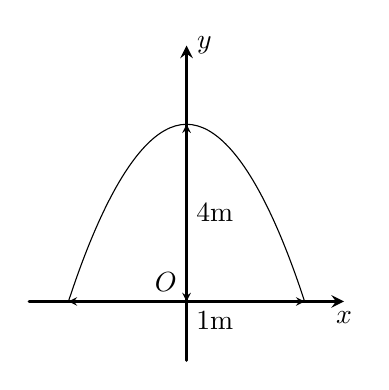
\begin{tikzpicture}[scale=1, line join=round, line cap=round,>=stealth]
				\draw[->,line width = 1pt] (-2,-2.25)--(-2,-2.25)--(2,-2.25) node[below]{$x$};
				\draw[->,line width = 1pt] (0,-3) --(0,1) node[right]{$y$};
				\draw [<->] (1.5,-2.25)--(-1.5,-2.25);
				\draw [<->] (0,0)--(0,-2.25);
				\draw (0,-1.125) node[right]{$4 \mathrm{m}$};
				\draw (0,-2.25) node[below right]{$1 \mathrm{m}$} ;
				\draw (0,-2.25) node[above left]{$O$} ;
				\draw (0,0) parabola (1.5,-2.25) ;
				\draw (0,0) parabola (-1.5,-2.25) ;
			\end{tikzpicture}	
		}
		\noindent Thể tích phần không gian lối đi giới hạn giữa hai cửa là $ 8\cdot \dfrac{8}{3}=\dfrac{64}{3}\approx 21{,}3$ m$^3$.
	}
\end{ex}

% #3837 | Archive/SP_KhoLatex/SP_Đề Theo Bài-Khối 12/2-B13-De2.tex | mã gốc 2D4C3-2
\begin{ex}%[ST12-dot1-Trần xuân Hòa]%[2D4C3-2]
	\immini{Một hoa văn trang trí được tạo ra từ một miếng bìa hình vuông cạnh bằng $10$ cm bằng cách khoét đi bốn phần bằng nhau có hình dạng parabol như hình vẽ bên. Biết $ AB=5$ cm, $OH=4$ cm. Tính diện tích của bề mặt hoa văn đó (đơn vị: cm$^2$) (kết quả làm tròn đến chữ số thập phân thứ nhất).
		\shortans{$46{,}7$}
	}{\begin{tikzpicture}[scale=0.9, font=\footnotesize, line join=round, line cap=round,>=stealth]
			\tikzset{label style/.style={font=\footnotesize}}
			\def \r{0.5*sqrt(3)};
			\coordinate (A) at ($(2,{\r})$);
			\coordinate (B) at ($(2,{-\r})$);
			\coordinate (H) at ($(A)!0.5!(B)$);
			\clip(-2,-2) rectangle (2.5,2);
			\fill [black] (-2,-2) rectangle (2,2);
			\foreach \i in {0,90,180,270}
			\draw [rotate=\i, fill=white,smooth, samples=200]  plot [domain={-\r-0.01}:{\r+0.01}] (\x, {2*(\x)^2+0.5});
			\draw (A) node[right]{$ A $}--(B)node[right]{$ B $};
			\draw (0.5, 0) node[left]{$\color{white} O $}--(H)node[right]{$H$};
	\end{tikzpicture}}
	\loigiai{
		Diện tích bề mặt hoa văn là $ S=10^2-4S_0 $, trong đó $ S_0 $ là diện tích của Parabol.
		\immini{Chọn hệ trục tọa độ như hình vẽ bên.\\
			Parabol có đỉnh $ O(0; 0) $ và đi qua điểm $ B\left(\dfrac{5}{2}; 4\right) $ nên có phương trình là $ y=\dfrac{16}{25}x^2 $.\\
			Tính $S_0$. Ta có $S_0=4\cdot 5-2\cdot \displaystyle\int\limits_{0}^{\tfrac{5}{2}}\dfrac{16}{25}x^2\mathrm{\, d}x=\dfrac{40}{3}$ (cm$^2$).
			}{
			\begin{tikzpicture}[scale=0.7, font=\footnotesize, line join=round, line cap=round,>=stealth]
				\def \xmin{-3.1}
				\def \xmax{3.1}
				\def \ymin{-1.9}
				\def \ymax{5.3}
				\draw[->] (\xmin, 0.) -- (\xmax,0.) node[anchor=north] {$x$};
				\draw[->] (0.,\ymin) -- (0.,\ymax) node[anchor=west] {$y$};
				\clip(\xmin,\ymin) rectangle (\xmax,\ymax);
				\draw[smooth,samples=100,domain=\xmin:\xmax] plot(\x,{0.64*(\x)^2});
				\draw[pattern=north west lines,smooth,samples=100,domain=-2.5:2.5] plot(\x,{0.64*(\x)^2});
				\draw[dashed] (-2.5,0) node[below] {$-\dfrac{5}{2}$} -- (-2.5,4)node[left]{$ A $}--(0,4)node[above left] {$4$}--(2.5,4)node[right]{$ B $}--(2.5,0)node[below]{$ \dfrac{5}{2} $};
				\draw(0,4)node[above right]{$ H $};
				\draw[fill=black] (0,0) circle (1.5pt) node[below left] {$O$};
		\end{tikzpicture}}\noindent
		Vậy diện tích bề mặt hoa văn là $ S=100-4\cdot\dfrac{40}{3}=\dfrac{140}{3}\approx 46{,}7$ (cm$^2$).
	}
\end{ex}

% #3860 | Archive/SP_KhoLatex/SP_Đề Theo Bài-Khối 12/2-OTC4-De2.tex | mã gốc 2D4V2-6
\begin{ex}%[2D4V2-6]
	Giả sử $v(t)$ là phương trình vận tốc của một vật chuyển động theo thời gian $t$ (giây), $a(t)$ là phương trình gia tốc của vật đó chuyển động theo thời gian $t$ (giây). Xét chuyển động trong khoảng thời gian từ $c$ (giây) đến $b$ (giây).
	\choiceTF
	{\True $\displaystyle\int\limits_c^b a(t)\mathrm{\,d}t=v(b)-v(c)$}
	{$\displaystyle\int\limits_c^b v(t)\mathrm{\,d}t=a(b)-a(c)$}
	{$\displaystyle\int\limits_c^b v'(t)\mathrm{\,d}t=v(c)-v(b)$}
	{\True $\displaystyle\int\limits_c^b v'(t)\mathrm{\,d}t=v(b)-v(c)$}
	\loigiai
	{
		\begin{itemchoice}
		\itemch $\displaystyle\int\limits_c^b a(t)\mathrm{\,d}t=v(b)-v(c)$ đúng do $v=a'$.
		\itemch $\displaystyle\int\limits_c^b v(t)\mathrm{\,d}t=a(b)-a(c)$ sai do $\displaystyle\int v = s+C$.
		\itemch $\displaystyle\int\limits_c^b v'(t)\mathrm{\,d}t=v(c)-v(b)$ sai do ngược cận.
		\itemch $\displaystyle\int\limits_c^b v'(t)\mathrm{\,d}t=v(b)-v(c)$ đúng do $\displaystyle\int v' = v+C$.
		\end{itemchoice}
		Là những khẳng định đúng.
	}
\end{ex}

% #3861 | Archive/SP_KhoLatex/SP_Đề Theo Bài-Khối 12/2-OTC4-De2.tex | mã gốc 2D4V2-6
\begin{ex}%[2D4V2-6]
Một vật chuyển động với gia tốc $a(t)=2\cos t$ (m/s$^2$).
	\choiceTF
	{\True Tại thời điểm bắt đầu chuyển động, vật có vận tốc bằng $0$. Khi đó, vận tốc của vật được biểu diễn bởi hàm số $v(t)=2\sin t$ (m/s)}
	{Vận tốc của vật tại thời điểm $t=\dfrac{\pi}{2}$ là $1$ m/s}
	{\True Quãng đường vật đi được từ thời điểm $t=0$ (s) đến thời điểm $t=\pi$ (s) là $4$ m}
	{Quãng đường vật đi được từ thời điểm $t=\dfrac{\pi}{2}$ (s) đến thời điểm $t=\dfrac{3\pi}{4}$ (s) là $2$ m}
	\loigiai{
		\begin{itemchoice}
	\itemch Ta có $v(t)=\displaystyle\int a(t) \mathrm{\,d}t=\displaystyle\int 2\cos t \mathrm{\,d}t=2\sin t+C$. \\
	Mà tại thời điểm bắt đầu chuyển động, vật có vận tốc bằng 0 nên ta có $v(0)=0$ hay $C=0$. \\
	Vậy $v(t)=2\sin t$.
\itemch Vận tốc của vật tại thời điểm $t=\dfrac{\pi}{2}$ là $v\left(\dfrac{\pi}{2}\right)=2\sin \dfrac{\pi}{2}=2$ (m/s).
\itemch Quãng đường vật đi được từ thời điểm $t=0$ (s) đến thời điểm $t=\pi$ (s) là
		$$
		\displaystyle\int_0^\pi v(t) \mathrm{\,d}t=\displaystyle\int_0^\pi 2 \sin t \mathrm{\,d}t=-\left.2 \cos t\right|_0 ^\pi=-2 \cos \pi-(-2 \cos 0)=4\,(\mathrm{m}).
		$$
	\itemch  Quãng đường vật đi được từ thời điểm $t=\dfrac{\pi}{2}$ (s) đến thời điểm $t=\dfrac{3\pi}{4}$ (s) là
		$\displaystyle\int_{\frac{\pi}{2}}^{\frac{3 \pi}{4}} v(t) \mathrm{\,d}t
		=\displaystyle\int_{\frac{\pi}{2}}^{\frac{3 \pi}{4}} 2 \sin t \mathrm{\,d}t
		=-2 \cos t\Big| _{\frac{\pi}{2}} ^{\frac{3 \pi}{4}}
		=-2 \cos \dfrac{3\pi}{4}-\left(-2 \cos \dfrac{\pi}{2}\right)
		=\sqrt{2}\,(\mathrm{m}).$
	\end{itemchoice}
		}
\end{ex}

% #3865 | Archive/SP_KhoLatex/SP_Đề Theo Bài-Khối 12/2-OTC4-De2.tex | mã gốc 2D4V2-6
\begin{ex}%[2D4V2-6]
	Một vật chuyển động với gia tốc được cho bởi hàm số $a(t)=5\cos t$ (m/s$^2$). Lúc bắt đầu chuyển động vật có vận tốc $2{,}5$ m/s. Tính gia tốc của vật (đơn vị m/s$^2$) tại thời điểm vận tốc đạt giá trị lớn nhất trong $\pi$ (s) đầu tiên.
	\shortans{$0$}
	\loigiai{
		Vận tốc của vật được biểu diễn bởi hàm số $v(t)=\displaystyle\int a(t) \mathrm{\,d}t=\displaystyle\int 5\cos t \mathrm{\,d}t=5\sin t+C$.\\
		Khi bắt đầu chuyển động, vật có vận tốc $2{,}5$ m/s nên ta có
		$$
		v(0)=2{,}5 \Leftrightarrow 5 \sin 0+C=2{,}5 \Leftrightarrow C=2{,}5
		$$
		Suy ra $v(t)=5\sin t+2{,}5$. \\
		Ta có $\sin t \le 1 \Rightarrow 5\sin t+2{,}5\leq 7{,}5$. \\
		Vận tốc đạt giá trị lớn nhất khi $\sin t=1 \Rightarrow t=\dfrac{\pi}{2}$. \\
		Khi đó, gia tốc của vật tại thời điểm $t=\dfrac{\pi}{2}$ là $a\left(\dfrac{\pi}{2}\right)=5\cos \left(\dfrac{\pi}{2}\right)=0$ m/s$^2$}
\end{ex}

% #3867 | Archive/SP_KhoLatex/SP_Đề Theo Bài-Khối 12/2-OTC4-De2.tex | mã gốc 2D4V3-2
\begin{ex}%[2D4V3-2]
	\immini{Bạn An cần mua một chiếc gương có viền là đường parabol bậc $2$ (xem hình vẽ). Biết rằng đoạn $AB=60$ cm, $OH=30$ cm. Diện tích của chiếc gương bạn An mua bằng bao nhiêu cm$^2$?
	\shortans{$1200$}
	}{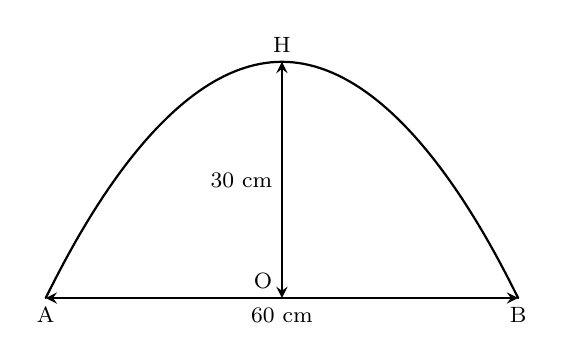
\begin{tikzpicture}[scale=1,font=\footnotesize,line join = round, line cap = round, >= stealth]
			%\tkzDefPoints{0/0/A, 5/0/x, 1.5/1/y, 0/5/z}
			\draw[thick] (-3,0) parabola bend (0,3) (3,0);
			\draw[thick,<->] (-3,0)--(3,0);
			\draw[thick,<->] (0,0)--(0,3);
			\draw (0,3) node[above]{H} (-3,0) node[below]{A} (3,0) node[below]{B} (0,0) node[above left]{O};
			\draw (0,0) node[below]{$60$ cm};
			\draw[](0,1.5) node[left]{$30$ cm};
			%\clip (-3.5,-1) rectangle (3.5,3.5);
	\end{tikzpicture}}
	\loigiai{
		\immini{Xét hệ trục tọa độ $Oxy$, sao cho gốc $O$ trùng với điểm $O$, trục $Ox$ trùng với tia $OB$, trục $Oy$ trùng với tia $OH$.\\
			Khi đó $B(30;0)$, $H(0;30)$.\\
			Phương trình Parabol đi qua $A$, $H$, $B$ có dạng\\ $y=ax^2+b\quad(P)$.
		}{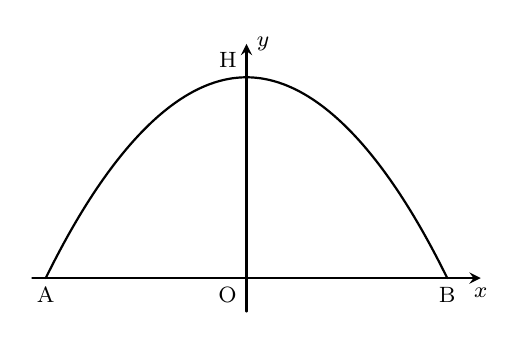
\begin{tikzpicture}[scale=.85,font=\footnotesize,line join = round, line cap = round, >= stealth]
				%\tkzDefPoints{0/0/A, 5/0/x, 1.5/1/y, 0/5/z}
				\draw[thick] (-3,0) parabola bend (0,3) (3,0);
				\draw[thick,->] (-3.2,0)--(3.5,0) node[below]{$x$};
				\draw[thick,->] (0,-0.5)--(0,3.5) node[right]{$y$} ;
				\draw (0,3) node[above left]{H} (-3,0) node[below]{A} (3,0) node[below]{B} (0,0) node[below left]{O};
				%\draw (0,0) node[below]{$60$ cm};
				%\draw[](0,1.5) node[left]{$30$ cm};
				%\clip (-3.5,-1) rectangle (3.5,3.5);
		\end{tikzpicture}}
		\noindent $H\in (P)\Rightarrow 30=b.\quad(1)$\\
		$B\in (P)\Rightarrow 0=a\cdot 30^2+30\Rightarrow a =-\dfrac{1}{30}.\quad(2)$\\
		Từ $(1)$, $(2)\Rightarrow (P)\colon y=-\dfrac{1}{30}x^2+30$.\\
		Diện tích của chiếc gương là
		\[\displaystyle\int\limits_{-30}^{30}\left(-\dfrac{1}{30}x^2+30\right)\mathrm{\,d}x=\left.\left(-\dfrac{x^3}{90}+30x\right)\right|_{-30}^{30}=1200\, \text{(cm$^2$)}.\]
	}
\end{ex}

% #3882 | Archive/SP_KhoLatex/SP_Đề Theo Bài-Khối 12/2-B12-De2.tex | mã gốc 2D4H2-6
\begin{ex}%[2D4H2-6]
	Một ô tô đang chạy với tốc độ $10$ m/s thì người lái đạp phanh, từ thời điểm đó ô tô chuyển động chậm dần đều với vận tốc $v(t)=-5t+10$ m/s, trong đó $t$ là khoảng thời gian tính bằng giây, kể từ lúc bắt đầu đạp phanh. Hỏi từ lúc đạp phanh đến khi dừng hẳn, ô tô còn di chuyển bao nhiêu mét?
	\shortans[]{$10$}
	\loigiai{
		Thời điểm ô tô dừng hẳn là $v(t)=-5t+10=0\Leftrightarrow t=2 $ s.\\
		Từ lúc đạp phanh đến khi dừng hẳn, ô tô còn di chuyển được là
		\allowdisplaybreaks
		\begin{eqnarray*}			S=\displaystyle\int\limits_{0}^{2}v(t)\mathrm{\,d}t=\displaystyle\int\limits_{0}^{2}(-5t+10)\mathrm{\,d}t=\left.\left(-\dfrac{5t^2}{2}+10t\right)\right|_{0}^{2}=10\, (\text{m}).
		\end{eqnarray*}
	}
\end{ex}

% #3901 | Archive/SP_KhoLatex/SP_Đề Theo Bài-Khối 12/2-OTC4-De1.tex | mã gốc 2D4V2-6
\begin{ex}%[2D4V2-6]%Biên soạn:Phùng Hoàng Em %Phản biện:Nguyễn Đắc Kiên
	\immini[thm]{ Một vật chuyển động trong $4$ giờ với vận tốc $v$ (km/h) phụ thuộc 
		thời gian $t$ (h) có đồ thị của vận tốc như hình bên. Trong khoảng thời gian $3$ giờ kể từ khi bắt đầu chuyển động, đồ thị đó là một phần của đường parabol có đỉnh $I(2;9)$ với trục đối xứng song song với trục tung, khoảng thời gian còn lại đồ thị là một đoạn thẳng song song với trục hoành.
		\choiceTF
		{\True Vận tốc lớn nhất của chuyển động là $9$ (km/h)}
		{\True $v(t)=-\dfrac{9}{4}t^2+9t$, với $0 \le t \le 3$}
		{$v(t)=\dfrac{27}{4}t$, với $3 \le t \le 4$}
		{\True Quãng đường vật di chuyển được trong $4$ giờ là $27$ km}
	}{
		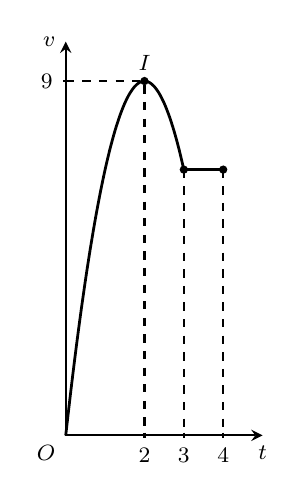
\begin{tikzpicture}[>=stealth,x=1.0cm,y=1.0cm,scale=0.5,thick]
			\draw[<->] (0,10) node[left]{\footnotesize $v$}--(0,0)--(5,0) node[below] {\footnotesize $t$};
			\foreach \x in {2,3,4}
			\draw[shift={(\x,0)},color=black] (0pt,2pt) -- (0pt,-2pt) node[below] {\footnotesize $\x$};
			\foreach \y in {9}
			\draw[shift={(0,\y)},color=black] (2pt,0pt) -- (-2pt,0pt) node[left] {\footnotesize $\y$};
			\draw (0,0) node[below left] {\footnotesize $O$};
			\draw[line width=1.0pt,color=black,smooth,domain=0:3] plot(\x,{-9*(\x)^2/4+9*\x});
			\draw[dashed] (0,9)--(2,9)--(2,0) (3,6.75)--(3,0) (4,6.75)--(4,0);
			\draw[line width=1.0pt,color=black] (3,6.75)--(4,6.75);
			\fill[black] (2,9) circle[radius=3pt] node[above]{\footnotesize $I$}(3,6.75) circle[radius=3pt] (4,6.75) circle[radius=3pt];
		\end{tikzpicture}
	}
	\loigiai{
		\begin{itemchoice}
			\itemch Dựa vào đồ thị của hàm vận tốc trên miền $t \in [0;4]$ thì $v_{\max}=9$ (km/h) khi $t=2$.
			\itemch Trên đoạn $t \in [0;3]$ thì đồ thị $v(t)$ là một parabol có đỉnh là $I(2;9)$ nên phương trình của nó có dạng $y=a(t-2)^2+9.$ Do parabol đi qua gốc tọa độ nên \[a(0-2)^2+9=0 \Leftrightarrow 4a+9=0 \Leftrightarrow a =-\dfrac{9}{4}.\]
			Vậy trên đoạn $[0;3]$ thì $v(t)=-\dfrac{9}{4}t^2+9t$.
			\itemch Với $t=3$ thì $v=\dfrac{27}{4}$. Trên đoạn $t \in [3;4]$ thì phần đồ thị là đường thẳng song song với trục hoành, suy ra $v(t)=\dfrac{27}{4}$ khi $t \in[3;4]$.
			\itemch Quãng đường mà vật di chuyển được trong $4$ giờ là
			$$s=\displaystyle\int\limits_0^3 \left (-\dfrac{9}{4}t^2+9t \right )\mathrm{\, d}t+\int\limits_3^4\dfrac{27}{4}\mathrm{\, d}t=27 \,\text{km}. $$
		\end{itemchoice}
	}
\end{ex}

% #3905 | Archive/SP_KhoLatex/SP_Đề Theo Bài-Khối 12/2-OTC4-De1.tex | mã gốc 2D4V2-6
\begin{ex}%[2D4V2-6]%Biên soạn:Phùng Hoàng Em %Phản biện:Nguyễn Đắc Kiên
	Giá trị trung bình của hàm số liên tục $f(x)$ trên đoạn $[a ; b]$ được định nghĩa là
	$$
	\dfrac{1}{b-a} \int_a^b f(x) \mathrm{\,d}x .
	$$
	Giả sử nhiệt độ ngoài trời ở một thành phố vào các thời điểm khác nhau trong ngày được mô phỏng bởi công thức $	h(t)=29+3 \sin \left[\dfrac{\pi}{12}(t-9)\right]$, với $h$ tính bằng độ $\mathrm{C}$ và $t$ là thời gian trong ngày tính bằng giờ.	Tìm nhiệt độ trung bình (đơn vị: độ) của ngày trong khoảng thời gian từ $6$ giờ sáng đến $12$ giờ trưa.
	\shortans{$29$}
	\loigiai{
	Nhiệt độ trung bình của ngày trong khoảng thời gian $6\le t \le 12$ được tính bởi công thức sau
\[\dfrac{1}{12-6} \int_6^{12} h(t) \mathrm{\,d}t=\dfrac{1}{6} \int_6^{12} \left( 29+3 \sin \left[\dfrac{\pi}{12}(t-9)\right]\right) \mathrm{\,d}t=29.\]
}
\end{ex}

% #3906 | Archive/SP_KhoLatex/SP_Đề Theo Bài-Khối 12/2-OTC4-De1.tex | mã gốc 2D4C2-6
\begin{ex}%[2D4C2-6]%Biên soạn:Phùng Hoàng Em %Phản biện:Nguyễn Đắc Kiên
Tại một nhà máy sản xuất một loại phân bón, gọi $P(x)$ là lợi nhuận (tính theo triệu đồng) thu được từ việc bán $x$ tấn sản phẩm trong một tuần. Khi đó, đạo hàm $P^{\prime}(x)$, gọi là lợi nhuận cận biên, cho biết tốc độ tăng lợi nhuận theo lượng sản phẩm bán được. Giả sử lợi nhuận cận biên (tính theo triệu đồng trên tấn) của nhà máy được ước lượng bởi công thức
$$
P^{\prime}(x)=16-0{,}02 x \text { với } 0 \leq x \leq 100.
$$
Tính lợi nhuận (triệu đồng) nhà máy thu được khi bán $90$ tấn sản phẩm trong tuần. Biết rằng nhà máy lỗ $25$ triệu đồng nếu không bán được lượng sản phẩm nào trong tuần.
	\shortans{$1334$}
\loigiai{
	Ta có $P(0)=-25$ (lỗ khi không bán được lượng sản phẩm nào trong tuần)
	$$
	\begin{aligned}
		P(90)-P(0) &=\displaystyle\int\limits_0^{90} P^{\prime}(x) \mathrm{\,d}x=\displaystyle\int\limits_0^{90}(16-0{,}02 x) \mathrm{\,d} x \\
		&=16 \displaystyle\int\limits_0^{90} \mathrm{\,d} x-0{,}02 \displaystyle\int\limits_0^{90} x \mathrm{\,d} x \\
		&=\left.16 x\right|_0 ^{90}-0{,}01 x^2\left.\right|_0 ^{90}=1359.
	\end{aligned}
	$$
	Suy ra $P(90)=P(0)+1359=-25+1359=1334$ (triệu đồng).\\
	Vậy lợi nhuận nhà máy thu được khi bán $90$ tấn sản phẩm trong tuần là $1334$ triệu đồng.
}
\end{ex}

% #3915 | Archive/SP_KhoLatex/SP_Đề Theo Bài-Khối 12/2-B12-De1.tex | mã gốc 2D4V2-6
\begin{ex}%[2D4V2-6]
    Tại một nơi không có gió, một chiếc khí cầu đang đứng yên ở độ cao 162 (m) so với mặt đất đã được phi công cài đặt cho nó chế độ chuyển động đi xuống. Biết rằng, khí cầu đã chuyển động theo phương thẳng đứng với vận tốc tuân theo quy luật $v(t)=10 t-t^2$, trong đó $t$ (phút) là thời gian tính từ lúc bắt đầu chuyển động, $v(t)$ được tính theo đơn vị mét/phút (m/p). Nếu như vậy thì khi bắt đầu tiếp đất vận tốc $v$ của khí cầu bằng bao nhiêu m/p?
    \shortans{$9$}
    \loigiai{
    Gọi thời điểm khí cầu bắt đầu chuyển động là $t=0$, thời điểm khinh khí cầu bắt đầu tiếp đất là $t_1$.\\
    Quãng đường khí cầu đi được từ thời điểm $t=0$ đến thời điểm khinh khí cầu bắt đầu tiếp đất $t=t_1$ là
    $$
    \begin{aligned}
    	& \displaystyle\int\limits_0^{t_1}\left(10 t-t^2\right) \mathrm{\,d} t=5 t_1^2-\dfrac{t_1^3}{3}=162 \\
    	& \Leftrightarrow t \approx-4{,}93 \vee t \approx 10{,}93 \vee t=9.
    \end{aligned}
    $$
    Do vận tốc chuyển động $v(t) \geq 0 \Leftrightarrow 0 \leq t \leq 10$ nên chọn $t_1=9$.\\
    Vậy khi bắt đầu tiếp đất vận tốc $v$ của khí cầu là $v(9)=10\cdot9-9^2=9$ m/p.	
    }
\end{ex}

% #3916 | Archive/SP_KhoLatex/SP_Đề Theo Bài-Khối 12/2-B12-De1.tex | mã gốc 2D4V2-6
\begin{ex}%[2D4V2-6]
    Gọi $h(t)$ cm là mức nước trong bồn chứa sau khi bơm được $t$ giây. Biết rằng tốc độ tăng giảm của mực nước là $h^{\prime}(t)=\dfrac{1}{5} \sqrt[3]{t+8}$ (cm/s) và lúc đầu bồn không có nước. Tìm mức nước ở bồn (đơn vị: cm) sau khi bơm nước được $6$ giây (làm tròn đến chữ số hàng phần trăm).
    \shortans{$2{,}66$}
    \loigiai{Hàm $h(t)=\displaystyle\int\limits \dfrac{1}{5} \sqrt[3]{t+8} \mathrm{\,d} t=\dfrac{3}{20}(t+8) \sqrt[3]{t+8}+C$.\\
        Lúc $t=0$, bồn không chứa nước. Suy ra $h(0)=0 \Rightarrow \dfrac{12}{5}+C=0 \Leftrightarrow C=-\dfrac{12}{5}$.\\
        Vậy, hàm $h(t)=\dfrac{3}{20}(t+8) \sqrt[3]{t+8}-\dfrac{12}{5}$.\\
        Mức nước trong bồn sau $6$ giây là $h(6) \simeq 2{,}66$ cm.
        }
\end{ex}

% #3917 | Archive/SP_KhoLatex/SP_Đề Theo Bài-Khối 12/2-B12-De1.tex | mã gốc 2D4C2-6
\begin{ex}%[2D4C2-6]
    Một vật chuyển động với vận tốc tăng liên tục được biểu thị bằng đồ thị là đường cong parabol ở hình bên dưới.
        \begin{center}
        \begin{tikzpicture}[>=stealth]
	\draw[->] (-0.5,0) --(0,0) node[below
	right]{$O$} -- (5,0)
	node[below]{$t(s)$};
	\draw[->](0,-0.5)--(0,5)
	node[right]{$v(m)$};
	\draw[smooth,blue,line width=1]
	plot[domain=0:4]
	(\x,{-(\x)^(2)+4*\x});
         \draw[dashed] (0,4) node[left]{} -- (2,4) --(2,0);
        \draw (2,0) node[below] {$10$};
        \draw (0,4) node[left] {$50$};
         \end{tikzpicture}
         \end{center} 
    Biết rằng sau $10$s thì vật đó đạt đến vận tốc cao nhất và bắt đầu giảm tốc. Hỏi từ lúc bắt đầu đến lúc đạt vận tốc cao nhất thì vật đó đi được quãng đường bao nhiêu mét (làm tròn đến chữ số hàng đơn vị)?
    \shortans{333}
         \loigiai{Giả sử vận tốc của vật biểu diển bởi hàm số $(P)\colon v(t)=a t^2+b t+c \quad(a \neq 0)$.\\
         Dựa vào đồ thị hàm số ta có $(P)$ đi qua $O(0 ; 0)$ và có đỉnh $I(10 ; 50)$.
        $$
        \Rightarrow \heva{& 
         c = 0  \\ &
        1 0 0 a + 1 0 b = 5 0 \\&
         - \dfrac { b } { 2 a } = 1 0 }
         \Rightarrow
         \heva {&      
        c = 0  \\&
        1 0 a + b = 5 \\&
        2 0 a + b = 0 }
        \Rightarrow
       \heva {&
        c=0 \\&
        a=-\dfrac{1}{2} \\&
        b=10}
        \Rightarrow (P) \colon v(t)=-\dfrac{1}{2} t^2+10 t.$$
         Lúc bắt đầu: $t=0$ s; lúc đạt vận tốc cao nhất: $t=10$ s.\\
         Vậy quãng đường vận đó đi được kể từ lúc bắt đầu đến lúc đạt vận tốc cao nhất là
         $$s=\displaystyle\int\limits_0^{10} v(t) \mathrm{\,d} t=\displaystyle\int\limits_0^{10}\left(-\dfrac{1}{2} t^2+10 t\right) \mathrm{\,d} t=\dfrac{1000}{3}\simeq 333.$$
        }
\end{ex}

% #4010 | Archive/SP_KhoLatex/SP_Đề Theo Bài-Khối 12/2-OTCK2-De2.tex | mã gốc 2D4H3-3
\begin{ex}%[Nguyễn Tuấn, dự án sáng tác đề 12]%[2D4H3-3]
	\immini
	{
		Một vật trang trí có dạng khối tròn xoay tạo thành khi quay miền $(R)$ được giới hạn bởi đường gấp khúc $DABFE$ và cung tròn $ED$ (phần gạch chéo trong hình bên) xung quanh trục $AB$. Biết $ABCD$ là hình chữ nhật cạnh $AB =3$ cm, $AD=2$ cm; $F$ là trung điểm của $BC$; điểm $E$ cách $AD$ một đoạn bằng $1$ cm. Tính thể tích của vật trang trí đó, làm tròn kết quả đến hàng phần mười, đơn vị cm$^3$.
		\shortans{$16{,}5$}
	}
	{
		\begin{tikzpicture}[scale=1.2, line join=round, line cap=round,>=stealth,font=\footnotesize]
			\path (0,0) coordinate (B)	(2,0) coordinate (C) (2,3) coordinate (D) (0,3) coordinate (A) ($(B)!.5!(C)$) coordinate (F) ($(F)+(0,2)$) coordinate (E) ($(A)!.5!(D)$) coordinate (I) ;
			\draw (A)--(B)--(C)--(D)--cycle (E)--(F);
			\draw[dashed] (E)--(I);
			\foreach \d/\g in {A/90,B/-90,C/0,D/90,F/-90,E/-60}
			\draw[fill=black] (\d) circle (1pt) +(\g:0.2) node{$\d$};
			\draw (E) arc (-90:0:1cm); 
			\fill[color=gray,opacity=0.5] (A)--(B)--(F)--(I)--cycle (E) arc (-90:0:1cm)--(D)--(I)--cycle;
		\end{tikzpicture}
	}
	\loigiai{
		\immini
		{
			Gắn hệ trục tọa độ như hình vẽ bên.\\
			Quay hình chữ nhật $GEFB$ xung quanh trục $AB$ ta được khối trụ có bán kính đáy bằng $1$ và chiều cao bằng $2$.\\
			Phương trình đường tròn tâm $I$ bán kính bằng $1$ là $x^2+(y-1)^2=1$, suy ra phương trình của cung $DE$ là $y=1+\sqrt{1-x^2}$.\\
			Vây thể tích của vật trang trí là
			$$V=\pi \displaystyle\int\limits_{0}^{1} \left(1+\sqrt{1-x^2}\right)^2 \mathrm{\,d}x+\pi \cdot 1^2\cdot 2\approx 16{,}5\ (\mathrm{cm}^3).$$
		}
		{
			\begin{tikzpicture}[scale=1.2, line join=round, line cap=round,>=stealth,font=\footnotesize]
				\draw[->] (-0.5,0)--(4,0) node[below]{$x$};
				\draw[->] (0,-0.5)--(0,3) node[left]{$y$};
				\path (0,0) coordinate (A)	(3,0) coordinate (B) (3,2) coordinate (C) (0,2) coordinate (D) ($(B)!.5!(C)$) coordinate (F) ($(F)-(2,0)$) coordinate (E) ($(A)!.5!(D)$) coordinate (I) (1,0) coordinate (G) ;
				\draw (A)--(B)--(C)--(D)--cycle (E)--(F);
				\draw[dashed] (E)--(I) (E)--(G);
				\foreach \d/\g in {A/-120,B/-90,C/0,D/120,F/0,E/-60,I/180,G/-90}
				\draw[fill=black] (\d) circle (1pt) +(\g:0.2) node{$\d$};
				\draw (E) arc (0:90:1cm); 
				\fill[color=gray,opacity=0.5] (A)--(B)--(F)--(I)--cycle (E) arc (0:90:1cm)--(D)--(I)--cycle;
			\end{tikzpicture}	
		}
	}
\end{ex}

% #4026 | Archive/SP_KhoLatex/SP_Đề Theo Bài-Khối 12/2-B11-De1.tex | mã gốc 2D4V1-6
\begin{ex}%[Đề 12 - 2025 - Nguyen Son]%[2D4V1-6]
	\immini{
		Một vật chuyển động trong 4 giờ với vận tốc $v$ (km/h) phụ thuộc thời gian $t$ (h) có đồ thị của vận tốc như hình bên. Trong khoảng thời gian 3 giờ kể từ khi bắt đầu chuyển động, đồ thị đó là một phần của parabol có đỉnh $I\left(2;9\right)$ với trục đối xứng song song với trục tung, khoảng thời gian còn lại đồ thị là một đoạn thẳng song song với trục hoành.
	}{
		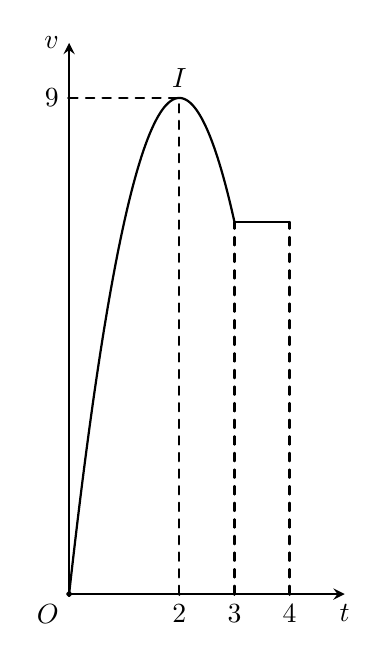
\begin{tikzpicture}[line join=round, line cap=round,>=stealth,thick,scale=0.7]
			
			\draw[->] (0,0)--(5,0) node[below] {$t$};
			\draw[->] (0,0)--(0,10) node[left] {$v$};
			\draw (0,0) node [below left] {$O$} circle(1pt);
			\draw[dashed] (2,0) -- (2,9) -- (0,9) (3,0)--(3,6.75) (4,0)--(4,6.75);
			\draw[samples=200,domain=0:3,smooth,variable=\x] plot (\x,{(-2.25)*(\x)^2 +9*(\x)});
			\draw[thick] (3,6.75)--(4,6.75);
			\fill 
			(0,9) node[left]{$9$} circle(1pt)
			(2,0) node[below]{$2$} circle(1pt)
			(3,0) node[below]{$3$} circle(1pt) 
			(4,0)node[below]{$4$} circle (1pt)
			(2,9)node[above]{$I$};
	\end{tikzpicture}}
	\choiceTF
	{\True Vận tốc lớn nhất của chuyển động là $9$ (km/h)}
	{\True $v(t)=-\dfrac{9}{4}t^2+9t$, với $0\leq t\leq 3$}
	{$v(t)=\dfrac{27}{4}t$, với $3\leq t\leq 4$}
	{\True Quãng đường vật di chuyển được trong 4 giờ là $27$ km}
	\loigiai{		
		\begin{itemchoice}
			\itemch Đúng. Dựa vào đồ thị hàm số ta có $\max\limits_{\left[0;4\right]}v=9$ khi $t=2$ h.
			\itemch Đúng. Với $0\leq t\leq 3$ ta có đồ thị vận tốc là một parabol. Vì parabol có đỉnh $I\left(2;9\right)$ nên parabol có phương trình dạng $y=a\left(t-2\right)^2+9$.\\
			Ta lại có parabol luôn đi qua gốc tọa độ nên $0=a(0-2)^2+9\Leftrightarrow a=-\dfrac{9}{4}$.\\
			Khi đó $y=-\dfrac{9}{a}\left(t-2\right)^2+9\Leftrightarrow y=-\dfrac{9}{4}t^2+9t$.
			\itemch Sai. Với $3\leq t\leq 4$ ta có đồ thị vận tốc là một đường thẳng song song với trục hoành nến $v=c$ với $c=v(3)=-\dfrac{9}{4}\cdot 3^2+9\cdot 3=\dfrac{27}{4}$.\\
			Vậy $y=\dfrac{27}{4}$ với $3\leq t\leq 4$.
			\itemch Đúng. Trong 4 giờ đầu vật chia thành 2 giai đoạn chuyển động.\\
			Giai đoạn 1, trong 3 giờ đầu ta có $s(t)=\displaystyle\int \left(-\dfrac{9}{4}t^2+9t\right)\mathrm{d}t=-\dfrac{3}{4}t^3+\dfrac{9}{2}t^2+c$.\\
			Vì $s(0)=0$ nên $c=0$. Suy ra, $s_{1}=s(3)=\dfrac{81}{4}$ km.\\
			Giai đoạn 2, từ giờ thứ 3 đến giờ thứ 4, ta có $s(t)=\displaystyle\int \dfrac{27}{4}\mathrm{d}t=\dfrac{27}{4}t+c'$. Vì $s(3)=\dfrac{81}{4}$ nên $c'=0$.\\ Suy ra, $s_2=s(4)-s(3)=\dfrac{27}{4}$.\\
			Vậy $s=s_1+s_2=27$ km.
		\end{itemchoice}
	}
\end{ex}

% #4030 | Archive/SP_KhoLatex/SP_Đề Theo Bài-Khối 12/2-B11-De1.tex | mã gốc 2D4V1-6
\begin{ex}%[Đề 12 - 2025 - Nguyen Son]%[2D4V1-6]
	Một vật chuyển động có gia tốc là $a\left(t\right)=3 t^2+t$ (m/s$^2$). Biết rằng vận tốc ban đầu của vật là $2$ m/s. Vận tốc của vật đó sau $4$ giây là bao nhiêu (m/s)?
	\shortans{$74$}
	\loigiai{
		Vận tốc của vật là $v(t)=\displaystyle \int \left(3 t^2+t\right)  \mathrm{\,d}t =t^3+\dfrac{1}{2}t^2+C$.\\
		Vì vận tốc tốc ban đầu của vật là $2$ m/s nên $v(0)=2 \Leftrightarrow 0^3+\dfrac{1}{2}\cdot 0^2+C=2  \Leftrightarrow C=2$.\\
		Suy ra $v(t)=t^3+\dfrac{1}{2}t^2+2$.\\
		Vận tốc của vật đó sau $4$ giây là $v(4)=4^3+\dfrac{1}{2}\cdot 4^2+2=74$ (m/s).
	}
\end{ex}

% #4058 | Archive/SP_KhoLatex/SP_Đề Theo Bài-Khối 12/2-B11-De2.tex | mã gốc 2D4V1-6
\begin{ex}%[2D4V1-6]%[2015_K12 Huyên Nguyễn]
	Một vận động viên điền kinh chạy với gia tốc $a(t)=-\dfrac{1}{24}t^3+\dfrac{5}{16}t^2$ (m/s$^2$), trong đó $t$ là khoảng thời gian tính từ lúc xuất phát.
	\choiceTF
	{ Vận tốc của vận động viên được tính theo công thức $v(t)=-\dfrac{1}{96}t^4+\dfrac{5}{48}t^3+3t$ m/s}
	{\True Vận tốc của vận động viên tại giây thứ $5$ là $6{,}51$ (m/s)}
	{Quãng đường chạy được của vận động viên sau thời gian $t$ giây được tính theo công thức $S(t)=-\dfrac{1}{480}t^5+\dfrac{5}{206}t^4$ (m)}
	{Sau $4$ giây thì vận động viên chạy được quãng đường là $6{,}2$ m}
	\loigiai{
		\begin{itemchoice}
			\itemch Sai.  $v(t)=\displaystyle\int a(t)\mathrm{\,d}t =\int \left( -\dfrac{1}{24}t^3+\dfrac{5}{16}t^2\right)\mathrm{\,d}t=-\dfrac{1}{96}t^4+\dfrac{5}{48}t^3+C$.\\
			Vì tại thời điểm $t=0$, vận tốc của vận động viên là $v(0)=0$ nên ta có\\ $v(t)=-\dfrac{1}{96}t^4+\dfrac{5}{48}t^3$ (m/s).
			\itemch Đúng. Tại giây thứ $5$ ta có 
			$v(5)=-\dfrac{1}{96}5^4+\dfrac{5}{48}5^3\approx 6{,}51$ m/s.
			\itemch Sai. Quãng đường chạy của vận động viên sau thời gian $t$ giây là 
			$$S(t)=\displaystyle\int v(t)\mathrm{\,d}t=\int \left( -\dfrac{1}{96}t^4+\dfrac{5}{48}t^3\right)\mathrm{\,d}t=-\dfrac{1}{480}t^5+\dfrac{5}{192}t^4+C.$$
			Tại thời điểm ban đầu $S(0)=0$ nên $S(t)=-\dfrac{1}{480}t^5+\dfrac{5}{192}t^4$ (m).
			\itemch Sai. Sau $4$ giây thì vận động viên chạy được quãng đường là\\ $S(4)=-\dfrac{1}{480}4^5+\dfrac{5}{192}4^4=\dfrac{68}{15}= 4{,}53$ m.
		\end{itemchoice}
	}
\end{ex}

% #4061 | Archive/SP_KhoLatex/SP_Đề Theo Bài-Khối 12/2-B11-De2.tex | mã gốc 2D4V1-6
\begin{ex}%[2D4V1-6]
	Một vật chuyển động có gia tốc là $a\left(t\right)=\dfrac{3}{t+1}$ (m/s$^2$). Biết rằng vận tốc ban đầu của vật là $6$ m/s. Vận tốc của vật đó sau $5$ giây là bao nhiêu m/s$^2$ (làm tròn kết quả đến hàng phần mười)?
	\shortans{$13{,}2$}
	\loigiai{
		Vận tốc của vật là $v(t)=\displaystyle \int a\left(t\right)  \mathrm{\,d}t =\int \dfrac{3}{t+1}\mathrm{\,d}t=3\ln |t+1|+C$.\\
		Vì vận tốc tốc ban đầu của vật là $6$ m/s nên $v(0)=6 \Leftrightarrow 3\ln 1+C=6  \Leftrightarrow C=6$.\\
		Suy ra $v(t)=3\ln |t+1| +6$.\\
		Vận tốc của vật đó sau $10$ giây là $v(10)=3\ln|10+1|+6\approx 13{,}2$ (m/s).
	}
\end{ex}

% #4167 | Archive/SP_KhoLatex/SP_Đề Theo Bài-Khối 12/2-OTC3-DE2.tex | mã gốc 2D3B1-4
\begin{ex}%[2D3B1-4]%[2D3H1-4]%[2D3V1-4]
	Thời gian luyện tập trong một ngày (tính theo giờ) của một số vận động viên được ghi lại ở bảng sau:
	\begin{center}
		\begin{tabular}{|c|c|c|c|c|c|}
			\hline Thời gian luyện tập (giờ) & {$[0 ; 2)$} & {$[2 ; 4)$} & {$[4 ; 6)$} & {$[6 ; 8)$} & {$[8 ; 10)$} \\
			\hline Số vận động viên & 3 & 8 & 12 & 12 & 4 \\
			\hline
		\end{tabular}
	\end{center}
	\choiceTF
	{Có tất cả $40$ vận động viên được khảo sát}
	{\True Khoảng biến thiên mẫu mẫu số liệu trên là $R=10$ (giờ)}
	{\True Tứ phân vị thứ hai của mẫu số liệu trên là $Q_2=\dfrac{65}{12}$}
	{Khoảng tứ phân vị của mẫu số liệu trên là $\Delta_Q=\dfrac{25}{48}$}
	\loigiai{
		\begin{itemchoice}
			\itemch Sai. Vì số vận động viên được khảo sát là $n=3+8+12+12+4=39$.
			\itemch Đúng. Vì khoảng biến thiên $R=10-0=10$ (giờ).
			\itemch Đúng. Vì tứ phân vị thứ hai của dãy số liệu $x_1 ; x_2 ; \ldots ; x_{39}$ là $x_{20} \in[4 ; 6)$. Do đó tứ phân vị thứ hai của mẫu số liệu ghép nhóm là
			$$
			Q_2=4+\dfrac{\dfrac{2\cdot 39}{4}-(3+8)}{12} \cdot(6-4)=\dfrac{65}{12}.
			$$
			\itemch Sai. Vì tứ phân vị thứ nhât của dãy số liệu $x_1 ; x_2 ; \ldots ; x_{39}$ là $x_{10} \in[2 ; 4)$. Do đó tứ phân vị thứ nhất của mẫu số liệu ghép nhóm là
			$$
			Q_1=2+\dfrac{\dfrac{1\cdot 39}{4}-3}{8} \cdot(4-2)=\dfrac{59}{16}.
			$$
			Tứ phân vị thứ ba của dãy số liệu $x_1 ; x_2 ; \ldots ; x_{39}$ là $x_{30} \in[6 ; 8)$. Do đó tứ phân vị thứ ba của mẫu số liệu ghép nhóm là
			$$
			Q_3=6+\dfrac{\dfrac{3 \cdot 39}{4}-(3+8+12)}{12} \cdot(8-6)=\frac{169}{24}.
			$$
			Vậy khoảng tứ phân vị $\Delta _ Q=Q_3-Q_1=\dfrac{169}{24}-\dfrac{59}{16}=\dfrac{161}{48}$.
		\end{itemchoice}
	}
\end{ex}

% #4168 | Archive/SP_KhoLatex/SP_Đề Theo Bài-Khối 12/2-OTC3-DE2.tex | mã gốc 2D3B1-4
\begin{ex}%[2D3B1-4]%[2D3H1-4]%[2D3V1-4]
	Bảng tần số ghép nhóm số liệu dưới đây thống kê cân nặng của 40 học sinh lớp 12A trong một trường trung học phổ thông (đơn vị: kilôgam).
	\begin{center}
		$\begin{array}{|c|c|c|}
			\hline \text { Nhóm } & \text { Tần số } & \begin{array}{c}
				\text { Tần số } \\
				\text { tích luỹ }
			\end{array} \\
			\hline[30 ; 40) & 2 & 2 \\
			{[40 ; 50)} & 10 & 12 \\
			{[50 ; 60)} & 16 & 28 \\
			{[60 ; 70)} & 8 & 36 \\
			{[70 ; 80)} & 2 & 38 \\
			{[80 ; 90)} & 2 & 40 \\
			\hline & n=40 & \\
			\hline
		\end{array}$
	\end{center}
	\choiceTF
	{\True Cân nặng trung bình của $40$ học sinh trên là $56$ kg}
	{Tứ phân vị thứ hai của mẫu số liệu trên là $Q_2=50$ kg}
	{Khoảng tứ phân vị của mẫu số liệu trên là $\Delta_Q=15$ kg}
	{\True Trong bảng số liệu trên học sinh có cân nặng khoảng $54$ kg chiếm nhiều nhất}
	\loigiai{
		\begin{itemchoice}
			\itemch Đúng. Vì cân nặng trung bình $$\bar{x}=\dfrac{35\cdot 2+45\cdot 10+55\cdot 16+65\cdot 8+75\cdot 2+85\cdot 2}{40}=56.$$
			\itemch Sai. Vì tứ phân vị thứ hai của dãy số liệu $x_1 ; x_2 ; \ldots ; x_{40}$ thuộc $[50 ; 60)$. Do đó tứ phân vị thứ hai của mẫu số liệu ghép nhóm là
			$$
			Q_2=50+\dfrac{\dfrac{2\cdot 40}{4}-(2+10)}{16} \cdot(60-50)=55.
			$$
			\itemch Sai. Vì tứ phân vị thứ nhất $Q_1=48$ (kg) và tứ phân vị thứ ba $Q_3=62{,}5$ (kg). \\
			Nên $\Delta_Q=62{,}5-48=14{,}5$.
			\itemch Đúng. Vì theo mẫu số liệu trên ta có mốt 
			$$M_{\circ}=50+\dfrac{16-10}{(16-10)+(16-8)}(65-50)=54{,}286.$$
		\end{itemchoice}
	}
\end{ex}

% #4169 | Archive/SP_KhoLatex/SP_Đề Theo Bài-Khối 12/2-OTC3-DE2.tex | mã gốc 2D3B2-3
\begin{ex}%[2D3B2-3]%[2D3H2-3]%[2D3V2-3]
	Thống kê tổng số giờ nắng trong tháng 9 tại một trạm quan trắc đặt ở Cà Mau trong các năm từ 2002 đến 2021 được thống kê như sau:
	\begin{center}
		\begin{tabular}{|c|c|c|c|c|c|}
			\hline Số giờ nắng & {$[80 ; 98)$} & {$[98 ; 116)$} & {$[116 ; 134)$} & {$[134 ; 152)$} & {$[152 ; 170)$} \\
			\hline Số năm & 3 & 6 & 3 & 5 & 3 \\
			\hline
		\end{tabular}
	\end{center}
	\begin{flushright}
		(\textit{Nguồn:} Tổng cục Thống kê)
	\end{flushright}
	\choiceTF
	{\True Giá trị đại diện của nhóm thứ ba là $125$ giờ}
	{\True Số giờ nắng trung bình của mẫu số liệu trên là $124{,}1$ giờ}
	{Tứ phân vị thứ hai của mẫu số liệu trên là $128$ giờ}
	{\True Độ lệch chuẩn của mẫu số liệu trên là $S=23{,}795$ giờ.}
	\loigiai{
		\begin{itemchoice}
			\itemch Đúng. Vì giá trị đại diện nhóm 3 bằng $\dfrac{134+116}{2}=125$ giờ.
			\itemch Đúng. Vì số giờ nắng trung bình của mẫu số liệu ghép nhóm là
			$$
			\bar{x}=\dfrac{3 \cdot 89+6 \cdot 107+3 \cdot 125+5 \cdot 143+3 \cdot 161}{20}=124{,}1 \text{ giờ.}
			$$
			\itemch Sai. Vì tứ phân vị thứ hai của dãy số liệu $x_1 ; x_2 ; \ldots ; x_{20}$ thuộc $[116 ; 134)$. Do đó tứ phân vị thứ hai của mẫu số liệu ghép nhóm là
			$$
			Q_2=116+\dfrac{\dfrac{2 \cdot 20}{4}-(3+6)}{3} \cdot(134-116)=122 \text{ giờ.}
			$$
			\itemch Đúng. Vì phương sai của mẫu số liệu ghép nhóm là
			$$
			S^2=\dfrac{1}{20}\left(3\cdot 89^2+6\cdot 107^2+3\cdot 125^2+5\cdot 143^2+3\cdot 161^2\right)-124,1^2=566{,}19.
			$$
			Độ lệch chuẩn của mẫu số liệu ghép nhóm là
			$$
			S=\sqrt{566{,}19} \approx 23{,}795.
			$$
		\end{itemchoice}
	}
\end{ex}

% #4170 | Archive/SP_KhoLatex/SP_Đề Theo Bài-Khối 12/2-OTC3-DE2.tex | mã gốc 2D3B2-3
\begin{ex}%[2D3B2-3]%[2D3H2-3]%[2D3V2-3]
	Giá đóng cửa của một cổ phiếu là giá của cổ phiếu đó cuối một phiên giao dịch. Bảng sau thống kê giá đóng cửa (đơn vị: nghìn đồng) của hai mã cổ phiếu $A$ và $B$ trong $50$ ngày giao dịch liên tiếp.
	\begin{center}
		\begin{tabular}{|c|c|c|c|c|c|}
			\hline Giá đóng cửa & {$[120 ; 122)$} & {$[122 ; 124)$} & {$[124 ; 126)$} & {$[126 ; 128)$} & {$[128 ; 130)$} \\
			\hline \begin{tabular}{c} 
				Số ngày giao dịch \\
				của cổ phiếu $A$
			\end{tabular} & 8 & 9 & 12 & 10 & 11 \\
			\hline \begin{tabular}{c} 
				Số ngày giao dịch \\
				của cổ phiếu $B$
			\end{tabular} & 16 & 4 & 3 & 6 & 21 \\
			\hline
		\end{tabular}
	\end{center}
	\choiceTF
	{\True Khoảng biến thiên trong mẫu số liệu trên bằng $10$ nghìn đồng}
	{\True Số trung bình của hai loại cổ phiếu trong mẫu số liệu trên là bằng nhau}
	{\True Độ lệch chuẩn trong mẫu số liệu của cổ phiếu A là $S_A\approx2{,}743$}
	{Nếu dùng phương sai và độ lệch chuẩn để so sánh mức độ rủi ro của các loại cổ phiếu có giá trị trung bình gần bằng nhau, cổ phiếu nào có phương sai, độ lệch chuẩn cao hơn thì được coi là có độ rủi ro lớn hơn. Như vậy thì cổ phiếu A sẽ có rủi ro cao hơn}
	\loigiai{
		\begin{itemchoice}
			\itemch Đúng. Vì khoảng biến thiên bằng $130-120=10$. 
			\itemch Đúng. Vì số trung bình của mẫu số liệu cổ phiếu A là
			$$
			\bar{x}_A=\dfrac{8 \cdot 121+9 \cdot 123+12 \cdot 125+10 \cdot 127+11 \cdot 129}{50}=125{,}28 .
			$$
			Số trung bình của mẫu số liệu cổ phiếu B là
			$$
			\bar{x}_B=\dfrac{16 \cdot 121+4 \cdot 123+3 \cdot 125+6 \cdot 127+21 \cdot 129}{50}=125{,}28 .
			$$
			\itemch Đúng. Vì phương sai của mẫu số liệu cổ phiếu A là
			$$
			S_A^2=\dfrac{1}{50}\left(8 \cdot 121^2+9 \cdot 123^2+12 \cdot 125^2+10 \cdot 127^2+11 \cdot 129^2\right)-(125{,}28)^2=7{,}5216 .
			$$
			Độ lệch chuẩn của mẫu số liệu cổ phiếu A là $S_A=\sqrt{S_A^2}=\sqrt{7{,}5216}\approx 2{,}743$.
			\itemch Sai. Vì độ lệch chuẩn của mẫu số liệu cổ phiếu B là $S_B=\sqrt{S_2^2}=\sqrt{12{,}4096}>S_A$.\\
			Vậy nếu đánh giá độ rủi ro theo phương sai và độ lệch chuẩn thì cổ phiếu $A$ có độ rủi ro thấp hơn cổ phiếu $B$.
		\end{itemchoice}
	}
\end{ex}

% #4257 | Archive/SP_KhoLatex/SP_Đề Theo Bài-Khối 12/2-OTGK2-De2.tex | mã gốc 2D4H2-6
\begin{ex}%[2D4H2-6] 
	Tốc độ chuyển động $v\,\mathrm{(m/s)}$ của ca nô trong khoảng thời gian $40$ giây được thể hiện như hình bên dưới. 
	\begin{center}
		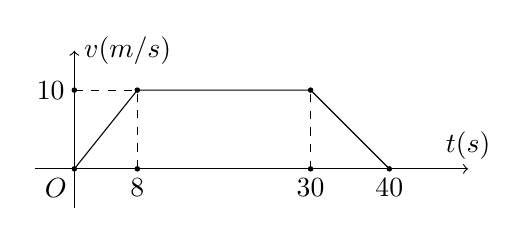
\begin{tikzpicture}
			\draw [->](-.5,0)node[below right]{$O$}--(5,0)node[above]{$t(s)$};
			\draw[->](0,-0.5)--(0,1.5)node[right]{$v(\text{m/s})$};
			\foreach \i /\t/\g in {(0,0),(0.8,0)/8/-90,(3,0)/30/-90,(4,0)/40/-90,(3,1)/ /0,(0.8,1)/ /0,(0,1)/10/180}{\fill \i circle(1pt);}
			\foreach \i /\t/\g in {(0.8,0)/8/-90,(3,0)/30/-90,(4,0)/40/-90,(3,1)/ /0,(0.8,1)/ /0}{	 \path \i node[below]{$\t$};}
			\path (0,1)node[left]{$10$};
			\draw (0,0)--(0.8,1)--(3,1)--(4,0);
			\draw[dashed](0,1)--(0.8,1)--(0.8,0) (3,0)--(3,1);
		\end{tikzpicture}
	\end{center}Quãng đường đi được (tính bằng m) của ca nô trong khoảng thời gian này là bao nhiêu?
	\shortans{$310$}
	\loigiai{
		Quãng đường đi được của ca nô trong $40$ giây là
			\begin{eqnarray*}
			S &=&
			\displaystyle\int\limits_{0}^{8} \dfrac{10}{8}x\mathrm{\,d}x+\displaystyle\int\limits_{8}^{30} 10\mathrm{\,d}x+\displaystyle\int\limits_{30}^{40} (-x+40)\mathrm{\,d}x\\
			&=&
			\dfrac{5x^2}{8}\bigg|_{0}^{8}+10x\bigg|_{8}^{30}+\left(-\dfrac{x^2}{2}+40x\right)\bigg|_{30}^{40}=310 \text{ m}.
		\end{eqnarray*}
	}
\end{ex}

% #4259 | Archive/SP_KhoLatex/SP_Đề Theo Bài-Khối 12/2-OTGK2-De2.tex | mã gốc 2D4C3-2
\begin{ex}%[2D4C3-2]
	\immini
	{Ông An xây dựng một sân bóng đá mini hình chữ nhật có chiều rộng $30$m và chiều dài $50$m. Để giảm bớt chi phí cho việc trồng cỏ nhân tạo, ông An chia sân bóng ra làm hai phần (tô đen và không tô đen) như hình bên. Phần tô đen gồm hai phần diện tích bằng nhau và đường cong $AIB$ là một parabol đỉnh $I$ được trồng cỏ nhân tạo với giá $130\,000$ đồng/m$^2$ và phần còn lại được trồng với giá $90\,000$ đồng/m$^2$. 
	}
	{\begin{tikzpicture}[scale=0.9, font=\footnotesize,line join=round, line cap=round, >=stealth]
			\coordinate (I) at (0,0);
			\coordinate (A) at (1.5,2.25);
			\coordinate (B) at ($(A)+(0,-4.5)$);
			\coordinate (C) at ($(B)+(-7.5,0)$);
			\coordinate (D) at ($(A)-(B)+(C)$);
			\coordinate (M) at ($(A)!1/2!(D)$);
			\coordinate (N) at ($(B)!1/2!(C)$);
			\coordinate (P) at ($(A)+(-1.5,0)$);
			\coordinate (Q) at ($(B)+(-1.5,0)$);
			\coordinate (R) at ($(D)+(1.5,0)$);
			\coordinate (S) at ($(C)+(1.5,0)$);
			\coordinate (td) at ($(D)+(0,0.3)$);
			\coordinate (dt) at ($(D)+(-0.3,0)$);
			\coordinate (ct) at ($(C)+(-0.3,0)$);
			\coordinate (tr) at ($(R)+(0,0.3)$);
			\coordinate (rp) at ($(R)+(0.3,0)$);
			\coordinate (I') at ($(R)!1/2!(S)$);
			\coordinate (g) at ($(I')+(0.3,0)$);
			\fill[gray]plot[domain=0:1.5](\x,{sqrt(3.375*(\x))})--(A)--plot[domain=1.5:0](\x,{-sqrt(3.375*(\x))})--cycle;
			\fill[gray](C)--(D)--plot[domain=-6:-4.5](\x,{sqrt(3.375*(-\x-4.5))})--plot[domain=-4.5:-6](\x,{-sqrt(3.375*(-\x-4.5))})--cycle;
			\draw (A)--(B)--(C)--(D)--cycle (M)--(N);
			\draw[dashed] (P)--(Q) (R)--(S);
			\draw[<->](td)--(tr);
			\node at ($(td)!1/2!(tr)$)[above]{$10$ m};
			\draw[<->](dt)--(ct);
			\node at ($(dt)!1/2!(ct)$)[above,rotate=90]{$30$ m};
			\draw[<->](rp)--(g);
			\node at ($(rp)!1/2!(g)$)[above,rotate=-90]{$15$ m};
			\foreach \x/\g in {A/90,B/-90,I/180,I'/-40}\draw[fill=black] (\x) circle (.05) +(\g:.5)node{\footnotesize$\x$};
	\end{tikzpicture}}
	\noindent
	Hỏi ông An phải trả bao nhiêu tiền (triệu đồng) để trồng cỏ nhân tạo cho sân bóng.
	\shortans{$151$}
	\loigiai{
		\immini{
			Chọn hệ trục tọa độ như hình vẽ ($I$ là gốc tọa độ). Khi đó đường cong $IAB$ là một parabol có phương trình dạng $y=ax^2$.\\
			Parabol đi qua điểm $\left(15;10 \right)$, suy ra 
			\[a \cdot 15^2=10 \Rightarrow a=\dfrac{2}{45}.\]
		}
		{
		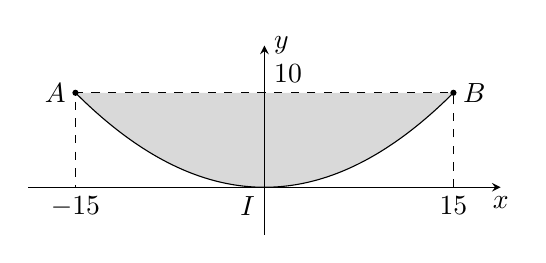
\begin{tikzpicture}[smooth,samples=300,scale=0.6,>=stealth]
			\fill[gray!30] (-4,2)--(4,2)--plot[domain=4:-4](\x,{0.125*(\x)^2});
			\draw[->] (-5,0)--(5,0) node[below]{$x$};
			\draw[->] (0,-1)--(0,3) node[right]{$y$};
			\draw (0,0) node[below left]{$I$};
			\draw[domain=-4:4] plot(\x,{0.125*(\x)^2});
			\draw[fill=black] (4,2) circle(1.5pt) (-4,2) circle(1.5pt);
			\draw[dashed] (4,0)node[below]{$15$}--(4,2)node[right]{$B$}--(-4,2)node[left]{$A$}--(-4,0)node[below]{$-15$};
			
			\node[right] at (0,2.4) {$10$};
	\end{tikzpicture}}
		\noindent
		Vậy $y=\dfrac{2}{45}x^2$. Diện tích phần tô đen là $S=2 \cdot \displaystyle\int\limits_{-15}^{15} \left(10-\dfrac{2}{45}x^2 \right) \mathrm{\,d}x=400 \, (\text{m}^2)$.\\
		Diện tích phần còn lại của sân bóng là $S_2=30 \cdot 50-400=1100\,(\text{m}^2).$\\
		Số tiền Ông An phải trả để trồng cỏ nhân tạo cho sân bóng là
		$$130000\times 400+90000\times 1100=151000000\text{ đồng}=151\text{ triệu đồng.}$$}
\end{ex}

% #4288 | Archive/SP_KhoLatex/SP_Bộ đề OTK12/SP_Data/2-OTCK1-De2.tex | mã gốc 2D4V1-3
\begin{ex}%[2D4V1-3]
	Cân nặng của một số lợn con mới sinh thuộc hai giống $A$ và $B$ được cho ở biểu đồ dưới đây (đơn vị: $\mathrm{kg}$).
	\begin{center}
		\begin{tikzpicture}[scale=1.2, font=\footnotesize, line join=round, line cap=round, >=stealth]
			\coordinate [label= left: $0$](O) at (0,0) ;
			\coordinate [label= left: (Số con)](y) at (0,6) ;
			\coordinate [label= below: (kg)](x) at (8,0) ;
			\foreach \i in {1,2,3,4,5}
			{\draw[-,color=gray!40] (0,\i)--(8,\i); }
			\draw (0,1)node[left]{$10$}(0,2)node[left]{$20$}(0,3)node[left]{$30$}(0,4)node[left]{$40$}(0,5)node[left]{$50$};
			%--------------------------------------------
			\foreach \i/\j/\a in 
			{0.4/0.8/8,1.2/1.3/13,2/2.8/28,2.8/1.4/14,3.6/3.2/32,4.4/2.4/24,	5.2/1.7/17,6/1.4/14}{
				\draw[] ($(\i,\j)+(0,0.2)$) node[scale=0.8]{$\a$};
			}
			%-----------------------------------------------
			\foreach \i/\j in 
			{0/0.8,1.6/2.8,3.2/3.2,4.8/1.7}{
				\fill[blue!50] (\i,0) rectangle+ (0.8,\j);
				\draw[thick] (\i,0) rectangle+ (0.8,\j);
			}
			%-----------------------------------------------	
			\foreach \i/\j in 
			{0.8/1.3,2.4/1.4,4/2.4,5.6/1.4}{
				\fill[pattern=north east lines] (\i,0) rectangle+ (0.8,\j);
				\draw[thick] (\i,0) rectangle+ (0.8,\j);
			}	
			%-----------------------------------------------
			\foreach \i/\j in 
			{0.4/[1{,}0;1{,}1),2/[1{,}1;1{,}2),3.6/[1{,}2;1{,}3),5.2/[1{,}3;1{,}4)}{
				\draw($(\i,0)+(0.5,0)$) node[below]{\j};
			}	
			\foreach \i/\j in {}{\draw (\i,\j) node[above]{\j};
			}			
			\draw[->,very thick] (O)--(x);
			\draw[->,very thick] (O)--(y);
			\fill[blue!50,draw] (5.5,4.2) rectangle (6,4.8);
			\fill[pattern=north east lines,draw] (5.5,3.2) rectangle (6,3.8);
			\draw (6,4.5) node [right]{Giống $A$};
			\draw (6,3.5) node [right]{Giống $B$};
			\draw (4,5.5) node [above]{\textbf{Cân nặng của một số lợn con mới sinh}};
		\end{tikzpicture}
	\end{center}
	Gọi $\Delta Q_1$, $\Delta Q_2$ lần lượt là giá trị khoảng tứ phân vị của lợn con giống $A$ và $B$. Tìm giá trị của $\Delta Q_2-\Delta Q_1$ (làm tròn kết quả đến hàng phần trăm). 
	\shortans[]{$0{,}03$}
	\loigiai{
		Cân nặng của lợn con giống $A$ và giống $B$ được thống kê như sau:
		\begin{center}
			\setlength{\extrarowheight}{2pt}
			\newcommand{\PreBackslash}[1]{\let\temp=\\#1\let\\=\temp}
			\let\PBS=\PreBackslash
			\begin{tabular}{|>{\PBS\centering}m{4cm}|>{\PBS\centering}m{2cm}|>{\PBS\centering}m{2cm}| >{\PBS\centering}m{2cm}|>{\PBS\centering}m{2cm}|}\hline
				\textbf{Cân nặng ($\mathrm{kg}$)} &$[1{,}0;1{,}1)$&$[1{,}1;1{,}2)$&$[1{,}2;1{,}3)$&$[1{,}3;1{,}4)$\\
				\hline
				\textbf{Giá trị đại diện}&$1{,}05$&$1{,}15$&$1{,}25$&$1{,}35$\\
				\hline
				\textbf{Số con giống $A$}&$8$&$28$&$32$&$17$\\
				\hline
				\textbf{Số con giống $B$}&$13$&$14$&$24$&$14$\\
				\hline
			\end{tabular}
		\end{center} 
		\begin{enumerate}[$\bullet$]
			\item Xét mẫu số liệu của giống lợn $A$.\\
			Ta có $n=85$ nên tứ phân vị thứ nhất thuộc nhóm $[1{,}1;1{,}2)$.\\
			Do đó $Q_1=1{,}1+\dfrac{\dfrac{85}{4}-8}{28}\cdot (1{,}2-1{,}1)=\dfrac{257}{224}$.\\
			Tứ phân vị thứ ba thuộc nhóm $[1{,}2;1{,}3)$.\\
			Do đó $Q_3=1{,}2+\dfrac{\dfrac{3\cdot 85}{4}-(8+28)}{32}\cdot (1{,}3-1{,}2)=\dfrac{1\,647}{1\,280}$.\\
			Vậy $\Delta Q_1=Q_3-Q_1=\dfrac{1\,249}{8\,960}.$
			\item Xét mẫu số liệu của giống lợn $B$.\\
			Ta có $n=65$ nên tứ phân vị thứ nhất thuộc nhóm $[1{,}1;1{,}2)$.\\
			Do đó $Q_1=1{,}1+\dfrac{\dfrac{65}{4}-13}{14}\cdot (1{,}2-1{,}1)=\dfrac{629}{560}$.\\
			Tứ phân vị thứ ba thuộc nhóm $[1{,}2;1{,}3)$.\\
			Do đó $Q_3=1{,}2+\dfrac{\dfrac{3\cdot 65}{4}-(13+14)}{24}\cdot (1{,}3-1{,}2)=\dfrac{413}{320}$.\\
			Vậy $\Delta Q_2=Q_3-Q_1=\dfrac{75}{448}$.\\
			Giá trị của $\Delta Q_2-\Delta Q_1\approx 0,03$.
		\end{enumerate}
	}
\end{ex}

% #4289 | Archive/SP_KhoLatex/SP_Bộ đề OTK12/SP_Data/2-OTCK1-De2.tex | mã gốc 2D4V2-2
\begin{ex}%[2D4V2-2]
	Thâm niên công tác của các công nhân hai nhà máy $A$ và $B$ được thống kê ở bảng dưới đây:
	\begin{center}
		\setlength{\extrarowheight}{2pt}
		\newcommand{\PreBackslash}[1]{\let\temp=\\#1\let\\=\temp}
		\let\PBS=\PreBackslash
		\begin{tabular}{|>{\PBS\centering}m{6cm}|>{\PBS\centering}m{1.5cm}|>{\PBS\centering}m{1.5cm}| >{\PBS\centering}m{1.5cm}|>{\PBS\centering}m{1.5cm}|>{\PBS\centering}m{1.5cm}|}\hline
			\textbf{Thâm niên công tác (năm)} &$[0;5)$&$[5;10)$&$[10;15)$&$[15;20)$&$[20;25)$\\
			\hline
			\textbf{Số công nhân nhà máy $A$}&$35$&$13$&$12$&$12$&$8$\\
			\hline
			\textbf{Số công nhân nhà máy $B$}&$14$&$26$&$24$&$11$&$5$\\
			\hline
		\end{tabular}
	\end{center}
	Gọi $S_A$, $S_B$ lần lượt là độ lệch chuẩn về thâm niên công tác của công nhân hai nhà máy $A$ và $B$. Tính giá trị của $S_A-S_B$ (làm tròn kết quả đến hàng phần trăm).
	\shortans[]{$1{,}48$}
	\loigiai{
		Thâm niên công tác của công nhân hai nhà máy $A$ và $B$ được thống kê như sau:
		\begin{center}
			\setlength{\extrarowheight}{2pt}
			\newcommand{\PreBackslash}[1]{\let\temp=\\#1\let\\=\temp}
			\let\PBS=\PreBackslash
			\begin{tabular}{|>{\PBS\centering}m{6cm}|>{\PBS\centering}m{1.5cm}|>{\PBS\centering}m{1.5cm}| >{\PBS\centering}m{1.5cm}|>{\PBS\centering}m{1.5cm}|>{\PBS\centering}m{1.5cm}|}
				\hline
				\textbf{Thâm niên công tác (năm)} &$[0;5)$&$[5;10)$&$[10;15)$&$[15;20)$&$[20;25)$\\
				\hline
				\textbf{Giá trị đại diện} &$2{,}5$&$7{,}5$&$12{,}5$&$17{,}5$&$22{,}5$\\
				\hline
				\textbf{Số công nhân nhà máy $A$}&$35$&$13$&$12$&$12$&$8$\\
				\hline
				\textbf{Số công nhân nhà máy $B$}&$14$&$26$&$24$&$11$&$5$\\
				\hline
			\end{tabular}
		\end{center}
		\begin{enumerate}[$\bullet$]
			\item Xét mẫu số liệu thâm niên công tác của công nhân nhà máy $A$.\\
			Thâm niên trung bình của công nhân nhà máy $A$ :
			$$\overline{x}_A=\dfrac{1}{80}\left(2{,}5\cdot 35+7{,}5\cdot 13+12{,}5\cdot 12+17{,}5\cdot 12+22{,}5\cdot8\right)=\dfrac{145}{16}.$$
			Phương sai về thâm niên của công nhân nhà máy $A$: $$S_A^2=\dfrac{1}{80}\left(2{,}5^2\cdot 35+7{,}5^2\cdot 13+12{,}5^2\cdot 12+17{,}5^2\cdot 12+22{,}5^2\cdot8\right)-\left(\dfrac{145}{16}\right)^2 =\dfrac{12\,735}{256}.$$
			Độ lệch chuẩn  về thâm niên của công nhân nhà máy $A$: $S_A=\sqrt{S_A^2}\approx 7{,}05$.
			\item Xét mẫu số liệu thâm niên công tác của công nhân nhà máy $B$.\\
			Thâm niên trung bình của công nhân nhà máy $B$ :
			$$\overline{x}_B=\dfrac{1}{80}\left(2{,}5\cdot 14+7{,}5\cdot 26+12{,}5\cdot 24+17{,}5\cdot 11+22{,}5\cdot5\right)=\dfrac{167}{16}.$$
			Phương sai về thâm niên của công nhân nhà máy $B$: $$S_B^2=\dfrac{1}{80}\left(2{,}5^2\cdot 14+7{,}5^2\cdot 26+12{,}5^2\cdot 24+17{,}5^2\cdot 11+22{,}5^2\cdot 5\right)-\left(\dfrac{167}{16}\right)^2 =\dfrac{7\,951}{256}.$$
			Độ lệch chuẩn  về thâm niên của công nhân nhà máy $B$: $S_B=\sqrt{S_B^2}\approx 5{,}57$.\\
			Giá trị của $S_A-S_B\approx 7{,}05-5{,}57\approx 1{,}48$.
		\end{enumerate}
	}
\end{ex}

% #4298 | Archive/SP_KhoLatex/SP_Bộ đề OTK12/SP_Data/2-OTCK1-De1.tex | mã gốc 2D3K1-4
\begin{ex}%[2D3K1-4]
Một học sinh ghi lại bảng phân bố tần số, tần suất ghép lớp của một mẫu số liệu như sau
\begin{center}
	\begin{tabular}{|c|c|c|c|c|c|c|}
		\hline
		\bf Lớp  & [1; 9] & [10; 19] & [20; 29] & [30; 39] & [40; 49] & \\
		\hline
		\bf Tần số & & & & & & $n$\\
		\hline
		\bf Tần suất (\%) & 12{,}5 & 0{,}0 & 50{,}0 & 25{,}0 & 12{,}5 & 100\\
		\hline
	\end{tabular}
\end{center}
Tuy nhiên, em đó quên ghi kích thước mẫu $n$. Biết rằng $n$ là số có $2$ chữ số và chữ số tận cùng là $2$. Tìm giá trị nhỏ nhất của $n$.
\shortans{$32$}
\loigiai{Hai lớp $[1;9]$ và $[40; 49]$ có tần số là $n \cdot 12{,}5\%=\dfrac{n}{8}$.\\			
	Lớp $[20; 29]$ có tần số là $n \cdot 50\%=\dfrac{n}{2}$.\\
	Lớp $[30; 39]$ có tần số là $n \cdot 25\%=\dfrac{n}{4}$.\\
	Vì tần số là các số nguyên dương nên $n$ phải chia hết cho $8; 4; 2$. \\
	Mà $n$ là số có $2$ chữ số, chữ số tận cùng là $2$ và nhỏ nhất nên $n=32$.
}
\end{ex}

% #4383 | Archive/SP-4Phan-Dot3/Data/KNTT_2-OTGK2_De04.tex | mã gốc 2D4V2-6
\begin{ex}%[2D4V2-6]
	Một vật chuyển động với vận tốc $v(t) = -t^2 + 4t$ m/s. Quãng đường đi được từ giây thứ $1$ đến giây thứ $3$ bao nhiêu mét (kết quả làm tròn đến hàng phần trăm)?
	\shortans{7{,}33}
	\loigiai
	{
		Ta có vận tốc $v(t) = -t^2 + 4t$.\\
		Suy ra, quãng đường đi được từ giây thứ $1$ đến giây thứ $3$ là
		$$S = \displaystyle \int\limits_{1}^{3} \left(-t^2 + 4t\right) \mathrm{d}t = \dfrac{22}{3} \approx 7{,}33 \text{ m}.$$
	}
\end{ex}

% #4384 | Archive/SP-4Phan-Dot3/Data/KNTT_2-OTGK2_De04.tex | mã gốc 2D4V3-5
\begin{ex}%[2D4V3-5]
	\immini{Mặt cắt thẳng đứng của một cái cổng có dạng một đường parabol với chiều cao $OH=4$ m (hình bên). Diện tích hình phẳng giới hạn bởi đường parabol và đoạn thẳng $AB$ bằng bao nhiêu mét vuông (làm tròn kết quả đến hàng phần mười)?
	}{
		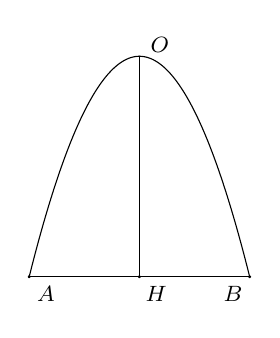
\begin{tikzpicture}[scale=0.7, font=\footnotesize, line join=round, line cap=round, >=stealth]
			
%			\draw[->] (-3,0)--(3,0) node[below left] {$x$};
%			\draw[->] (0,-5)--(0,1) node[below left] {$y$};
			\draw (0,0) node [shift={(30:3mm)}] {$O$};
			\draw[smooth, samples=200, domain=-2:2] plot(\x,{-(\x)^2});
			\draw (-2,-4)--(2,-4) (0,0)--(0,-4);
			\draw[fill=black] (-2,-4) circle(0.5pt) node[shift={(-45:3mm)}]{$A$};
			\draw[fill=black] (0,-4) circle(0.5pt) node[shift={(-45:3mm)}]{$H$};
			\draw[fill=black] (2,-4) circle(0.5pt) node[shift={(-135:3mm)}]{$B$};
		\end{tikzpicture}
	}
	\shortans{10{,}7}
	\loigiai
	{
		\immini{
			Chọn hệ trục tọa độ như hình bên.\\
			Đường cong đó có dạng $y=ax^2$. \\
			Đường cong đi qua điểm $(2,-4)$. Suy ra $a=-1$.\\
			Suy ra, đường cong có phương trình $y=-x^2$.\\
			Đường thẳng $AB \colon y=-4$.\\
			Diện tích mặt cắt là\\
			$S = 2\displaystyle \int\limits_{0}^{2} -x^2 +4\mathrm{d}x = 2\dfrac{16}{3} \approx 10{,}7$ m$^2$.
		}{
			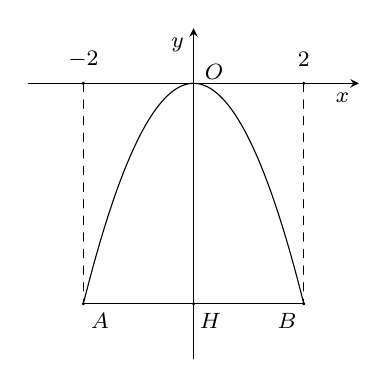
\begin{tikzpicture}[scale=0.7, font=\footnotesize, line join=round, line cap=round, >=stealth]
				
				\draw[->] (-3,0)--(3,0) node[below left] {$x$};
				\draw[->] (0,-5)--(0,1) node[below left] {$y$};
				\draw (0,0) node [shift={(30:3mm)}] {$O$};
				\draw[smooth, samples=200, domain=-2:2] plot(\x,{-(\x)^2});
				\draw (-2,-4)--(2,-4) (0,0)--(0,-4);
				\draw[fill=black] (-2,-4) circle(0.5pt) node[shift={(-45:3mm)}]{$A$};
				\draw[fill=black] (0,-4) circle(0.5pt) node[shift={(-45:3mm)}]{$H$};
				\draw[fill=black] (2,-4) circle(0.5pt) node[shift={(-135:3mm)}]{$B$};
				\draw[fill=black] (-2,0) circle(0.5pt) node[shift={(90:3mm)}]{$-2$};
				\draw[fill=black] (2,0) circle(0.5pt) node[shift={(90:3mm)}]{$2$};
				\draw[dashed] (-2,0)--(-2,-4) (2,0)--(2,-4);
			\end{tikzpicture}
		}
	}
\end{ex}

% #4385 | Archive/SP-4Phan-Dot3/Data/KNTT_2-OTGK2_De04.tex | mã gốc 2D4V3-5
\begin{ex}%[2D4V3-5]
	\immini{Anh Dũng đi rừng đào được tổ mối với mặt cắt có dạng như hình vẽ. Anh Dũng chú thích trên mặt cắt các kích thước. Đơn vị đo khoảng cách là dm. Tính diện tích mặt cắt của tổ mối. (Làm tròn kết quả đến hàng phần chục).
	}{
		\begin{tikzpicture}[scale=0.9, font=\footnotesize, line join=round, line cap=round, >=stealth]
			%			\draw[->] (-2.5,0)--(3.5,0) node[below left] {$x$};
			%			\draw[->] (0,-3)--(0,5) node[below left] {$y$};
			%			\draw (0,0) node [shift={(-130:3mm)}] {$O$};
			\draw[smooth, samples=200, domain=-1.3:-1,dashed] plot(\x,{(\x)^2-(\x)-2});
			\draw[smooth, samples=200, domain=-1:2] plot(\x,{(\x)^2-(\x)-2});
			\draw[smooth, samples=200, domain=2:2.5, dashed] plot(\x,{(\x)^2-(\x)-2});
			\draw[smooth, samples=200, domain=-1.2:-1, dashed] plot(\x,{(\x)^3-3*(\x)^2+4});
			\draw[smooth, samples=200, domain=-1:2] plot(\x,{(\x)^3-3*(\x)^2+4});
			\draw[smooth, samples=200, domain=2:2.5, dashed] plot(\x,{(\x)^3-3*(\x)^2+4});
			\draw[<->] (-1,0)--(0,0) node[sloped, pos=0.5, shift={(90:3mm)}]{$1$};
			\draw[<->] (0,0)--(2,0) node[sloped, pos=0.5, shift={(90:3mm)}]{$2$};
			\draw[<->] (0,0.5)--(1/2,0.5) node[sloped, pos=0.5, shift={(90:5mm)}]{$\dfrac{1}{2}$};
			\draw[<->] (0,0)--(0,4) node[sloped, pos=0.5, shift={(90:3mm)}]{$4$};
			\draw[<->] (1/2,-9/4)--(1/2,0) node[sloped, pos=0.7, shift={(-90:5mm)}]{$\dfrac{9}{4}$};
			\draw[dashed] (1/2,0)--(1/2,1/2);
		\end{tikzpicture}
	}
	 
	\shortans{11{,}3}
	\loigiai
	{
		\begin{center}
			\begin{tikzpicture}[scale=0.7, font=\footnotesize, line join=round, line cap=round, >=stealth]
				\draw[->] (-2.5,0)--(3.5,0) node[below left] {$x$};
				\draw[->] (0,-3)--(0,5) node[below left] {$y$};
				\draw (0,0) node [shift={(-130:3mm)}] {$O$};
				\draw[smooth, samples=200, domain=-1.3:-1,dashed] plot(\x,{(\x)^2-(\x)-2});
				\draw[smooth, samples=200, domain=-1:2] plot(\x,{(\x)^2-(\x)-2});
				\draw[smooth, samples=200, domain=2:2.5, dashed] plot(\x,{(\x)^2-(\x)-2});
				\draw[smooth, samples=200, domain=-1.2:-1, dashed] plot(\x,{(\x)^3-3*(\x)^2+4});
				\draw[smooth, samples=200, domain=-1:2] plot(\x,{(\x)^3-3*(\x)^2+4});
				\draw[smooth, samples=200, domain=2:2.5, dashed] plot(\x,{(\x)^3-3*(\x)^2+4});
				\draw[fill=black] (-1,0) circle(0.5pt) node[shift={(150:4mm)}]{$-1$};
				\draw[fill=black] (2,0) circle(0.5pt) node[shift={(-45:3mm)}]{$2$};
				\draw[fill=black] (0,4) circle(0.5pt) node[shift={(45:3mm)}]{$4$};
				\draw[fill=black] (1/2,0) circle(0.5pt) node[shift={(90:3mm)}]{$\tfrac{1}{2}$};
				\draw[fill=black] (0,-9/4) circle(0.5pt) node[shift={(180:3mm)}]{$-\tfrac{9}{4}$};
				\draw[dashed] (1/2,0)--(1/2,-9/4)--(0,-9/4);
			\end{tikzpicture}
		\end{center}
			Chọn hệ trục tọa độ như hình vẽ.\\
			Đường cong trên là đồ thị của hàm số bậc 3 $(C_1) \colon y=ax^3 + bx^2 + cx + d$.\\
			Có đạo hàm là $y'=3x^2+2bx+c$.\\
			$(C_1)$ đi qua điểm $(0;4)$ nên $d=4$.\hfill{$(1)$}\\
			$(C_1)$ đi qua điểm $(-1;0)$ nên $-a+b-c+d=0$.\hfill{$(2)$}\\
			$(C_1)$ đi qua điểm $(2;0)$ nên $8a+4b+2c+d=0$.\hfill{$(3)$}\\
			$(C_1)$ có điểm cực tiểu là $(0;4)$ nên $c=0$.\hfill{$(4)$}\\
			Từ $(1)$, $(2)$, $(3)$, $(4)$ suy ra $\hoac{&a=1\\&b=-3\\&c=0\\&d=4.}$\\
			Suy ra $(C_1) \colon y= x^3 - 3x^2 +4$.\\
			Mặt khác đường cong bên dưới là một parabol $(C_2) \colon y=ax^2+bx+c$.\\
			$(C_2)$ đi qua điểm $(-1,0)$ nên $a-b+c=0$. \hfill{$(5)$}\\
			$(C_2)$ đi qua điểm $(2,0)$ nên $4a+2b+c=0$. \hfill{$(6)$}\\
			$(C_2)$ đi qua điểm $\left(\dfrac{1}{2},-\dfrac{9}{4}\right)$ nên $\dfrac{1}{4}a+\dfrac{1}{2}b+c=-\dfrac{9}{4} \Leftrightarrow a + 2b +4c = -9$. \hfill{$(7)$}\\
			Từ $(5)$, $(6)$, $(7)$ suy ra $\hoac{&a=1\\&b=-1\\&c=-2.}$\\
			Suy ra $(C_2) \colon y= x^2 - x - 2$.
			Hai đồ thị $(C_1)$ và $(C_2)$ cắt nhau tại hai điểm $(-1,0)$ và $(2,0)$.
			Diện tích mặt cắt là\\
			$S = \displaystyle \int\limits_{-1}^{2} \left[\left(x^3 - 3x^2 +4\right) - \left(x^2 - x - 2\right)\right] \mathrm{d}x = \dfrac{45}{4} \approx 11{,}3$ dm$^2$.
	}
\end{ex}

% #4393 | Archive/SP-4Phan-Dot3/Data/KNTT_2-OTGK2_De03.tex | mã gốc 2D4V1-6
\begin{ex}%[2D4V1-6]
	Một viên đạn được bắn lên từ mặt đất theo phương thẳng đứng với vận tốc ban đầu là $25$ m/s. Biết gia tốc trọng trường là $9{,}8$ m/s$^2$. Hãy tính quãng đường viên đạn đi được từ lúc bắn lên cho đến khi chạm đất (kết quả làm tròn đến hàng phần chục).
	\shortans[]{$63{,}8$}
	\loigiai{
		Vì viên đạn được bắn lên trên với gia tốc là $9{,}8$ m/s$^2$ nên gia tốc có phương trình là $a(t)=-9{,}8$.\\
		Vận tốc là nguyên hàm của gia tốc nên phương trình vận tốc là $v(t)=\displaystyle\int a(t)\mathrm{\,d}t=-9{,}8t+C$.\\
		Theo đề $v(0)=25$ nên $C=25$ hay $v(t)=-9{,}8+25$.\\
		Ta có quãng đường viên đạn đi được từ lúc bắn lên đến khi chạm đất bằng hai lần quảng đường từ lúc bắn lên đến khi đạt độ cao lớn nhất.\\
		Và viên đạn đạt độ cao lớn nhất khi $v(t)=0$ hay $-9{,}8t+25=0 \Leftrightarrow t=\dfrac{125}{49}$.\\
		Vậy quảng đường viên đạt đi được là 
		$$s=2\displaystyle\int\limits_0^{\tfrac{125}{49}}\left(-9{,}8t+25\right)\mathrm{\,d}t=\dfrac{3125}{49}\approx 63{,}8 \text{ (m) }.$$
	}
\end{ex}

% #4395 | Archive/SP-4Phan-Dot3/Data/KNTT_2-OTGK2_De03.tex | mã gốc 2D4V3-5
\begin{ex}%[2D4V3-5]
	\immini{
		Trên bức tường cần trang trí một hình phẳng dạng parabol đỉnh $S$ như hình vẽ, biết $OS=AB=4$ m, $O$ là trung điểm $AB$. Parabol trên được chia thành ba phần để sơn ba màu khác nhau với mức chi phí:
		\begin{itemize}
			\item Phần trên (phần kẻ sọc) giá $140\,000$ đồng/m$^2$;
			\item Phần giữa (hình quạt tâm $O$ bán kính $2$ m được tô đậm) giá $150\,000$ đồng/m$^2$;
			\item Phần còn lại giá $160\,000$ đồng/m$^2$.
		\end{itemize}
		Tổng chi phí để sơn cả ba phần là bao nhiêu triệu đồng (kết quả làm tròn đến hàng phần trăm)?
	}{
		\begin{tikzpicture}[scale=0.8, font=\footnotesize, line join=round, line cap=round,>=stealth]
			\def\xmin{-2.5} \def\xmax{2.5}
			\def\ymin{-0.5} \def\ymax{4.5} 			
			\draw[smooth,samples=300,domain=-2:2] plot(\x,{-(\x)^2+4});			
			\draw[smooth,samples=300,domain=-1.732:1.732] plot(\x,{(4-(\x)^2)^0.5});
			\draw[pattern=north east lines,opacity=0.5] (-1.732,1) plot[domain=-1.732:1.732] (\x, {-(\x)^2+4})--(0,0)--cycle;
			\fill[samples=100,domain=-1.732:1.732,gray!60] plot(\x,{(4-(\x)^2)^0.5})--(0,0)--cycle;			
			\node at (0,0) [below]{$O$};
			\node at (0,4) [above]{$S$};
			\draw[fill=black] (-2,0)circle (.5pt) node[left]{\footnotesize $A$};
			\draw[fill=black] (2,0)circle (.5pt) node[right]{\footnotesize $B$};		
			\draw (-1.732,1)--(0,0)--(1.732,1) (-2,0)--(2,0);
			\clip (\xmin+0.1,\ymin+0.1) rectangle (\xmax-0.1,\ymax-0.1);
		\end{tikzpicture}	
	}
	\shortans{$1{,}58$}
	\loigiai{
		Chọn hệ trục tọa độ $Oxy$ như hình vẽ.
		\begin{center}
			\begin{tikzpicture}[scale=0.8, font=\footnotesize, line join=round, line cap=round,>=stealth]
				\def\xmin{-2.5} \def\xmax{2.5}
				\def\ymin{-0.5} \def\ymax{4.5} 			
				\draw[smooth,samples=300,domain=-2:2] plot(\x,{-(\x)^2+4});				
				\draw[smooth,samples=300,domain=-1.732:1.732] plot(\x,{(4-(\x)^2)^0.5});
				\draw[pattern=north east lines,opacity=0.5] (-1.732,1) plot[domain=-1.732:1.732] (\x, {-(\x)^2+4})--(0,0)--cycle;
				\fill[samples=100,domain=-1.732:1.732,gray!60] plot(\x,{(4-(\x)^2)^0.5})--(0,0)--cycle;				
				\draw[->] (\xmin,0)--(\xmax,0) node [right]{$x$};
				\draw[->] (0,\ymin)--(0,\ymax) node [left]{$y$};
				\node at (0,0) [below right]{$O$};
				\node at (1.2,3) [right]{$(P)$};
				\node at (.5,1.5) [right]{$(C)$};
				\node at (0,4) [above right]{$S$};
				\node at (-1.732,1) [left]{$M$};
				\node at (1.732,1) [right]{$N$};
				\draw[fill=black] (-2,0)circle (.5pt) node[below left]{\footnotesize $A$};
				\draw[fill=black] (2,0)circle (.5pt) node[below right]{\footnotesize $B$};
				\draw[fill=black] (-2,0)circle (.5pt) node[above left]{\footnotesize $-2$};
				\draw[fill=black] (2,0)circle (.5pt) node[above right]{\footnotesize $2$};
				\draw[fill=black] (-1.732,0)circle (.5pt) node[below]{\footnotesize $-\sqrt{3}$};
				\draw[fill=black] (-1.732,0)circle (.5pt) node[below]{\footnotesize $-\sqrt{3}$};
				\draw[fill=black] (1.732,0)circle (.5pt) node[below]{\footnotesize $\sqrt{3}$};
				\draw[fill=black] (0,1)circle (.5pt) node[above right]{\footnotesize $1$};
				\draw[dashed] (-1.732,0)--(-1.732,1)--(1.732,1)--(1.732,0);
				\draw (-1.732,1)--(0,0)--(1.732,1);
				\clip (\xmin+0.1,\ymin+0.1) rectangle (\xmax-0.1,\ymax-0.1);
			\end{tikzpicture}
		\end{center}
		Ta có phương trình parabol $(P)$ là $y=-x^2+4$; phương trình cung $\mathop{MN}$ (một phần của đường tròn tâm $O$, bán kính $R=2$) là $y=\sqrt{4-x^2}$; phương trình đoạn $ON$ là $y=\dfrac{1}{\sqrt{3}}x$.\\
		Diện tích phần gạch sọc là $S_1=2\displaystyle\int\limits_0^{\sqrt{3}}\left(-x^2+4-\sqrt{4-x^2}\right)\mathrm{\,d}x$.\\
		Diện tích hình quạt là $S_2=2\displaystyle\int\limits_0^{\sqrt{3}}\left(\sqrt{4-x^2}-\dfrac{1}{\sqrt{3}}x\right)\mathrm{\,d}x$.\\
		Diện tích phần còn lại là $S_3=\displaystyle\int\limits_{-2}^{2}\left(4-x^2\right)\mathrm{\,d}x-S_1-S_2$.\\
		Tổng chi phí là $T=S_1\cdot0{,}14+S_2\cdot0{,}15+S_3\cdot0{,}16\approx1{,}58$ (triệu đồng).
	}
\end{ex}

% #4403 | Archive/SP-4Phan-Dot3/Data/KNTT_2-OTGK2_De02.tex | mã gốc 2D4V1-6
\begin{ex}%[2D4V1-6]
	Một ôtô đang chuyển động với vận tốc $20$ m/s thì người lái xe đạp phanh. Từ thời điểm đó, ôtô chuyển động chậm dần với vận tốc biến thiên theo thời gian được xác định bởi $v(t)=-4t+20$ m/s trong đó $t$ là khoảng thời gian tính bằng giây kể từ lúc người lái xe bắt đầu đạp phanh. Gọi $x$ m là quãng đường ôtô đi được từ lúc người lái xe bắt đầu đạp phanh đến khi xe dừng hẳn. Tìm $x$.
	
	\shortans{50}
	\loigiai{
		Ta có $v(t)=-4t+20$. Lúc đó
		$$s(t)=\displaystyle \int{v(t)\mathrm{\,d}t}=\displaystyle \int{(-4t+20)\mathrm{\,d}t}=-2t^2+20t+C.$$
		Tại thời điểm $t=0$, người lái xe bắt đầu đạp phanh. Ta có $s(0)=0\Rightarrow C=0$.\\
		Suy ra $s(t)=-2t^2+20t$.\\
		Tại thời điểm xe dừng hẳn ta có $v(t)=0\Rightarrow -4t+20=0\Rightarrow t=5$.\\
		Quãng đường ôtô đi được từ lúc người lái xe bắt đầu đạp phanh đến khi xe dừng hẳn là $x=s(5)=50$ m.
	}
\end{ex}

% #4405 | Archive/SP-4Phan-Dot3/Data/KNTT_2-OTGK2_De02.tex | mã gốc 2D4V3-4
\begin{ex}%[2D4V3-4]
	Chuẩn bị cho đêm hội diễn văn nghệ chào đón năm mới, bạn Lan đã làm một chiếc mũ \lq\lq cách điệu\rq\rq\,cho ông già Noel có dáng một khối tròn xoay. Mặt cắt qua trục của chiếc mũ như hình vẽ bên dưới. Biết rằng $OO'=6$\,cm, $OA=10$\,cm, $OB=20$\,cm. Đường cong $AB$ là một phần của parabol có đỉnh là điểm $B$. Thể tích của chiếc mũ là bao nhiêu cm$^3$ (làm tròn đến hàng đơn vị)?
	\begin{center}
		\begin{tikzpicture}[scale=1.0,font=\footnotesize,line join=round,line cap=round,>=stealth]
			% Vẽ hình chữ nhật đáy
			\draw (-2,0) rectangle (2,-1);
			\node at (2,0) [above right] {$A$};
			\node at (0,-1) [above right] {$O'$};
			\node at (0,0) [above right] {$O$};
			
			% Vẽ đường cong
			\draw[domain=-2:0,smooth,variable=\x,samples=100] plot ({\x},{0.5*(\x)^2+2.5*(\x)+3});
			\draw[domain=0:2,smooth,variable=\x,samples=100] plot ({\x},{0.5*(\x)^2-2.5*(\x)+3});
			\draw[-] (0,3) -- (0,-1);
			\node at (0,3) [above] {$B$};
			\fill (2,0) circle (1pt) (-2,0) circle (1pt)
			(0,-1) circle (1pt)
			(2,-1) circle (1pt) (-2,-1) circle (1pt)
			(0,0) circle (1pt)
			(0,3) circle (1pt);
		\end{tikzpicture}
	\end{center}
	\par
	\shortans{3142}
	
	\loigiai{
		Ta chọn hệ trục toạ độ $Oxy$ như hình vẽ sau.
		\begin{center}
			\begin{tikzpicture}[scale=1.0,font=\footnotesize,line join=round,line cap=round,>=stealth]
				% Vẽ hình chữ nhật đáy
				\draw (-1,2) rectangle (0,-2);
				\node at (0,-2) [right] {$A$};
				\node at (-1,0) [above right] {$O'$};
				\node at (0,0) [above right] {$O$};
				
				% Vẽ đường cong
				\draw[domain=0:3,smooth,variable=\x,samples=100] plot ({\x},{0.17*(\x)^2-1.17*(\x)+2});
				\draw[domain=0:3,smooth,variable=\x,samples=100] plot ({\x},{-0.17*(\x)^2+1.17*(\x)-2});
				\draw[-] (-1,0) -- (3,0);
				\node at (3,0) [above] {$B$};
				\draw[->] (-2,0)--(4,0) node[below]{$x$};
				\draw[->] (0,-2.5)--(0,2.5) node[left]{$y$};
				\fill (0,0) circle (1pt) (0,-2) circle (1pt)
				(0,2) circle (1pt) (3,0) circle (1pt)
				(-1,0) circle (1pt) (-1,2) circle (1pt)
				(-1,-2) circle (1pt);
			\end{tikzpicture}
		\end{center}
		Gọi $y=f(x)=ax^2+bx+c$ là hàm số có đồ thị là đường Parabol đi qua điểm $A(0;-10)$ và có đỉnh là $B(20;0)$.\\
		Lúc đó ta có $\heva{&a\cdot 0^2+b\cdot 0+c=-10\\&-\dfrac{b}{2a}=20\\&a\cdot 20^2+b\cdot 20+c=0}\Leftrightarrow\heva{&a=-\dfrac{1}{40}\\&b=1\\&c=-10.}$\\
		Suy ra $y=f(x)=-\dfrac{1}{40}x^2+x-10$.\\
		Thể tích phần tròn xoay giới hạn bởi đồ thị hàm số $y=f(x)$, trục tung và xoay quanh trục hoành là
		\[V_1=\pi\displaystyle\int\limits_{0}^{20} \left(\dfrac{-1}{40}x^2+x-10\right)^2\mathrm{d}x= 400\pi\,\mathrm{cm}^3.\]
		Thể tích phần trụ tròn phía dưới là 
		\[V_2=\pi \cdot 10^2 \cdot 6=600 \pi\,\mathrm{cm}^3.\]
		Thể tích của cái mũ là \[V=V_1+V_2=1\,000 \pi \approx 3\,142\,\mathrm{cm}^3.\]
	}
\end{ex}

% #4425 | Archive/SP-4Phan-Dot3/Data/KNTT_2-OTGK2_De01.tex | mã gốc 2D4V3-4
\begin{ex}%[2D4V3-4]%Câu 6
	\immini[thm]{Một bình chứa nước dạng như Hình bên có chiều cao là $\dfrac{3\pi }{2}$\,dm. Nếu lượng nước trong bình có chiều cao là $x$\,(dm) thì mặt nước là hình tròn có bán kính $\sqrt{2-\sin x}$\,(dm) với $0\leq x\leq \dfrac{3\pi }{2}$. Tính dung tích của bình (kết quả làm tròn đến hàng phần mười của đềximét khối).\\
		\shortans{$26{,}5$}
	}{
		\begin{tikzpicture}[scale=1, font=\footnotesize, line join=round, line cap=round, >=stealth]
			\draw (0,1.4) ellipse (0.6cm and 0.2cm);
			\draw[dashed] (-0.9,0) arc (180:0:0.9cm and 0.2cm);
			\draw (-0.9,0) arc (-180:0:0.9cm and 0.2cm);
			\draw[dashed] (-0.7,-1.5) arc (180:0:0.7cm and 0.2cm);
			\draw (-0.7,-1.5) arc (-180:0:0.7cm and 0.2cm);
			\draw (-0.6,1.4).. controls +(-60:0.5) and +(75:0.2)..(-0.9,0)..controls +(-105:1) and +(105:0.5)..(-0.7,-1.5);
			\draw (0.6,1.4).. controls +(-120:0.5) and +(105:0.2)..(0.9,0)..controls +(-75:1) and +(75:0.5)..(0.7,-1.5);
			\draw [dashed](0,0)--(0.9,0) (0,-1.5)--(0,0) node[pos=0.5,left]{$x$};
			\draw [->](0.9,1)--(0.3,0) node[pos=-0.2,right=-0.2]{$\sqrt{2-\sin x}$};
		\end{tikzpicture}
	}
	\loigiai{
		Diện tích của mặt nước hình tròn bán kính $R=\sqrt{2-\sin x}$\,(dm) là \[S(x)=\pi  R^2=\pi (2-\sin  x)\,(\mathrm{dm}^2).\]
		Dung tích của bình là
		\begin{eqnarray*}
			V&=&\displaystyle\int\limits_0^{\tfrac{3\pi }{2}}S(x)\mathrm{\,d}x\\
			&=&\displaystyle\int\limits_0^{\tfrac{3\pi }{2}}\pi  (2-\sin  x)\mathrm{\,d}x\\
			&=&\pi (2x+\cos  x)\Big|_0^{\tfrac{3\pi }{2}}\\
			&=&\pi (3\pi -1) \approx 26{,}5\,\left(\mathrm{dm}^3\right).
		\end{eqnarray*}
	}
\end{ex}

% #4426 | Archive/SP-4Phan-Dot3/Data/KNTT_2-OTGK2_De01.tex | mã gốc 2D4V3-5
\begin{ex}%[2D4V3-5]
	Người ta tạo ra mô hình một quả trứng ngỗng bằng cách quay hình phẳng giới hạn bởi đồ thị hàm số $y=\dfrac{1}{30}\sqrt{7569-400x^2}$ và trục hoành với $-4{,}35\leq x\leq 4{,}35$ quanh trục hoành. Tính thể tích quả trứng (đơn vị: cm$^3$), biết thể tích mô hình này xem như bằng thể tích quả trứng ngỗng và $x$, $y$ tính theo centimét (kết quả làm tròn đến hàng đơn vị).\\
	\shortans{$153$}
	\loigiai{
		Thể tích quả trứng ngỗng là
		\begin{eqnarray*}
			V&=&\pi  \int\limits_{-4{,}35}^{4{,}35}\dfrac{1}{900}\left(7569-400x^2\right)\mathrm{\,d}x=\dfrac{\pi }{900}\left.\left(7569x-\dfrac{400x^3}{3}\right)\right|_{-4{,}35}^{4{,}35}\\
			&=&\dfrac{21\,9501\pi }{4\,500}\approx 153~\left(\mathrm{cm}^3\right).
		\end{eqnarray*}
	}
\end{ex}

% #4427 | Archive/SP-4Phan-Dot3/Data/KNTT_2-OTGK2_De01.tex | mã gốc 2D4V2-6
\begin{ex}%[2D4V2-6]
	Các nhà kinh tế sử dụng đường cong Lorenz để minh họa sự phân phối thu nhập trong một quốc gia. Gọi $x$ là đại diện cho phần trăm số gia đình trong một quốc gia và $y$ là phần trăm tổng thu nhập, mô hình $y=x$ sẽ đại diện cho một quốc gia mà các gia đình có thu nhập như nhau. Đường cong Lorenz $y=f(x)$, biểu thị sự phân phối thu nhập thực tế. Diện tích giữa hai mô hình này, với $0\leq x\leq 100$, biểu thị \lq\lq sự bất bình đẳng về thu nhập \rq\rq \, của một quốc gia. Năm $2009$, đường cong Lorenz của Hoa Kỳ có thể được mô hình hóa bởi hàm số
	$$
	y=\left(0{,}00\,061x^2+0{,}0\,224x+1{,}666\right)^2,\,0\leq x\leq 100.
	$$
	Trong đó $x$ được tính từ các gia đình nghèo nhất đến giàu có nhất. Sự bất bình đẳng về thu nhập của Hoa Kì vào năm $2009$ có giá trị gần nhất với giá trị là bao nhiêu (kết quả làm tròn đến hàng đơn vị)?\\
	\shortans{$2\,086$}
	\loigiai{
		Sự bất bình đẳng về thu nhập của Hoa Kì vào năm 2009 là diện tích hình phẳng $S$ giới hạn bởi
		$$\heva{&y=x\\&y=\left(0{,}00\,061x^2+0{,}0\,224x+1{,}666\right)^2\\&x=0;x=100.}$$
		Suy ra
		$$S=\int  _0^{100}\left|\left(0{,}00\,061x^2+0{,}0\,224x+1{,}666\right)^2-x\right|\mathrm{\,d}x.$$
		Sử dụng máy tính cầm tay, ta được $S\approx2\,086$.}
\end{ex}

% #4436 | Archive/SP-4Phan-Dot3/Data/CD_2-OTGK2-De04.tex | mã gốc 2D4V1-6
\begin{ex}%[Dự án đề 4 phần]%[Đoàn Hùng]%[2D4V1-6]	
	Tại một lễ hội dân gian hàng năm, số lượng khách tham dự tại thời điểm $t$ giờ được biểu diễn bằng hàm số $Q(t)$, trong đó $t$ tính bằng giờ $(0\leq t \leq 14)$. Tốc độ thay đổi lượng khách tham dự theo thời gian được cho bởi hàm số $Q'(t)=8t^3-144t^2+576t$, $Q'(t)$ tính bằng khách/giờ. Sau $1$ giờ đã có $300$ người tham dự. Hỏi số lượng khách tham dự đông nhất trong vòng $14$ giờ là bao nhiêu?
	\shortans[oly]{$2650$}
	\loigiai{
		Ta có $\displaystyle\int\limits Q'(t)\mathrm{\,d}t=\displaystyle\int\limits \left(8t^3-144t^2+576t\right)\mathrm{\,d}t=2t^4-48t^3+288t^2+C$.\\
		Vậy số lượng khách tham quan được biểu diễn bằng hàm số $Q(t)=2t^4-48t^3+288t^2+C$, với $(0\leq t\leq 14)$.\\
		Ta có $Q(1)=300 \Rightarrow C=58$, suy ra $Q(t)=2t^4-48t^3+288t^2+58$.\\
		$Q'(t)=8t^3-144t^2+576t=0 \Leftrightarrow \hoac{& t=0 \\ & t=6\\&t=12.}$\\
		Bảng biến thiên
		\begin{center}
			\begin{tikzpicture}
				\tkzTabInit[espcl=2.5,lgt=1.5,nocadre]
				{$t$/0.7,$Q'(t)$/0.7,$Q(t)$/2.1}
				{$0$,$6$,$12$,$14$}
				\tkzTabLine{,+,0,-,0,+,}
				\tkzTabVar{-/$58$,+/$2\,650$,-/$58$,+/$1\,626$}
			\end{tikzpicture}
		\end{center}
		Vậy số lượng khách tham dự đông nhất trong vòng $14$ giờ là $2\,650$ khách sau $6$ giờ.	
	}
\end{ex}

% #4437 | Archive/SP-4Phan-Dot3/Data/CD_2-OTGK2-De04.tex | mã gốc 2D4V1-6
\begin{ex}%[Dự án đề 4 phần]%[Đoàn Hùng]%[2D4V1-6]
	\immini{Một vật chuyển động trong $4$ giờ với vận tốc $v$ (km/h) phụ thuộc vào thời gian $t$ (h) có đồ thị vận tốc là một đường parabol có đỉnh $I(3;10)$ và trục đối xứng vuông góc với trục hoành như hình vẽ. Tính quãng đường vật di chuyển được trong nửa thời gian sau của chuyển động đó (kết quả làm tròn đến hàng phần chục và tính theo đơn vị km).}
	{
		\begin{tikzpicture}[scale=0.4,>=stealth, font=\footnotesize, line join=round, line cap=round]
			\def\xmin{-3} \def\xmax{6}
			\def\ymin{-1} \def\ymax{11}
			\draw[->] (\xmin,0)--(\xmax,0) node [below]{$t$};
			\draw[->] (0,\ymin)--(0,\ymax) node [left]{$v$};
			\fill (0,0) circle (1pt) node[shift={(-135:2.5mm)}]{$O$};
			\clip (\xmin+0.1,\ymin+0.1) rectangle (\xmax-0.1,\ymax-0.1);
			\draw[smooth,red,samples=300,domain=(0:4)] plot(\x,{-(\x)^2+6*(\x)+1});	
			\foreach \x in {\xmin,...,\xmax}
			\draw (\x,-0.05)--(\x,0.05);
			\foreach \y in {\ymin,...,\ymax}
			\draw (-0.05,\y)--(0.05,\y);	
			\node at (3,0)[below]{$3$};
			\node at (0,1)[left]{$1$};
			\node at (0,10)[left]{$10$};
			\draw[dashed] (0,10)--(3,10)--(3,0);
			%\node at (-1,1)[shift={(70:2mm)}]{$ I $};
			%\draw[dashed]
			%(-1,0)node[below]{$ -1 $}|-(0,1)node[right]{$1$}	
			%	;	
		\end{tikzpicture}
	}
	\shortans[oly]{$19{,}3$}
	
	\loigiai{
		Dựa vào đồ thị ta tìm được vận tốc $v(t)=-t^{2}+6 t+1, t \in[0 ; 4]$.\\
		Quãng đường $s(t)$ vật di chuyển được trong thời gian $4$ giờ là một nguyên hàm của $v(t)$, với $t \in[0 ; 4]$\\
		Ta có $s(t)=\displaystyle\int\left(-t^{2}+6t+1\right) \mathrm{d}t=-\dfrac{t^{3}}{3}+3 t^{2}+t+C$.\\
		Quãng đường vật di chuyển được trong $2$ giờ đầu là $s(2)=\dfrac{34}{3}+C$ (km).\\
		Quãng đường vật di chuyển được trong $4$ giờ  là $s(4)=\dfrac{92}{3}+C$ (km).\\
		Quãng đường vật di chuyển được trong nửa thời gian sau của chuyển động là
		$$s(4)-s(2)=\dfrac{58}{3} \text{~(km)} \approx 19{,}3\text{~(km)}.$$}
	
\end{ex}

% #4438 | Archive/SP-4Phan-Dot3/Data/CD_2-OTGK2-De04.tex | mã gốc 2D4V2-6
\begin{ex}%[Dự án đề 4 phần]%[Đoàn Hùng]%[2D4V2-6]
	Một ô tô đang chạy thì người lái đạp phanh. Từ thời điểm đó, ô tô chuyển động chậm dần đều với vận tốc $v(t)=-12 t+36$ (m/s) trong đó $t$ là khoảng thời gian tính bằng giây, kể từ lúc bắt đầu đạp phanh. Từ lúc đạp phanh đến khi dừng hẳn, ô tô di chuyển được quãng đường là $s$ mét. Tính giá trị của $s$.
	\shortans[oly]{$54$}
	\loigiai
	{Thời gian từ lúc xe đạp phanh đến lúc dừng hẳn là $v(t)=0 \Leftrightarrow-12 t+36=0 \Leftrightarrow t=3(s)$.\\
		Từ lúc đạp phanh đến khi dừng hẳn, ô tô di chuyển được quãng đường là $$s=\displaystyle\int\limits_0^3(-12 t+36) \mathrm{\,d}t=54 (\text{m}).$$
	}
\end{ex}

% #4450 | Archive/SP-4Phan-Dot3/Data/CD_2-OTGK2-De01.tex | mã gốc 2D4V1-6
\begin{ex}%[2D4V1-6]
	Tại một lễ hội dân gian hàng năm, tốc độ thay đổi lượng khách tham dự được biểu diễn bằng hàm số $Q'(t)=8t^3-144t^2+576t$, trong đó $t$ tính bằng giờ $(0\leq t \leq 14)$, $Q'(t)$ tính bằng khách/giờ. Sau $1$ giờ đã có $300$ người có mặt. Hỏi số lượng khách tham dự đông nhất trong vòng $14$ là bao nhiêu?
	\shortans[oly]{$2\,650$}
	\loigiai{
		Ta có $\displaystyle\int\limits Q'(t)\mathrm{\,d}t=\displaystyle\int\limits \left(8t^3-144t^2+576t\right)\mathrm{\,d}t=2t^4-48t^3+288t^2+C$.\\
		Vậy số lượng khách tham quan được biểu diễn bằng hàm số $Q(t)=2t^4-48t^3+288t^2+C$, với $(0\leq t\leq 14)$.\\
		Ta có $Q(1)=300 \Rightarrow C=58$, suy ra $Q(t)=2t^4-48t^3+288t^2+58$.\\
		$Q'(t)=8t^3-144t^2+576t=0 \Leftrightarrow \hoac{& t=0 \\ & t=6\\&t=12.}$\\
		Bảng biến thiên
		\begin{center}
			\begin{tikzpicture}
				\tkzTabInit[espcl=2.5,lgt=1.5,nocadre]
				{$t$/0.7,$Q'(t)$/0.7,$Q(t)$/2.1}
				{$0$,$6$,$12$,$14$}
				\tkzTabLine{,+,0,-,0,+,}
				\tkzTabVar{-/$58$,+/$2650$,-/$58$,+/$1626$}
			\end{tikzpicture}
		\end{center}
		Vậy số lượng khách tham dự đông nhất trong vòng $14$ giờ là $2650$ khách.	
	}
\end{ex}

% #4467 | Archive/SP-4Phan-Dot3/Data/CD_2-OTGK2-De03.tex | mã gốc 2D4V2-6
\begin{ex}%[2D4V2-6]
	Giá trị trung bình của hàm số liên tục $f(x)$ trên đoạn $[a ; b]$ được định nghĩa là
	$$
	\dfrac{1}{b-a} \int_a^b f(x) \mathrm{\,d}x .
	$$
	Giả sử nhiệt độ ngoài trời ở một thành phố vào các thời điểm khác nhau trong ngày được mô phỏng bởi công thức $	h(t)=29+3 \sin \left[\dfrac{\pi}{12}(t-9)\right]$, với $h$ tính bằng độ $\mathrm{C}$ và $t$ là thời gian trong ngày tính bằng giờ.	Tìm nhiệt độ trung bình (đơn vị: độ) của ngày trong khoảng thời gian từ $6$ giờ sáng đến $12$ giờ trưa.
	\shortans[oly]{$29$}
	\loigiai{
		Nhiệt độ trung bình của ngày trong khoảng thời gian $6\le t \le 12$ được tính bởi công thức sau
		\[
			\dfrac{1}{12-6} \int_6^{12} h(t) \mathrm{\,d}t
			=\dfrac{1}{6} \int_6^{12} \left( 29+3 \sin \left[\dfrac{\pi}{12}(t-9)\right]\right) \mathrm{\,d}t
			=29.\]
	}
\end{ex}

% #4468 | Archive/SP-4Phan-Dot3/Data/CD_2-OTGK2-De03.tex | mã gốc 2D4V2-6
\begin{ex}%[2D4V2-6]
	Tại một nhà máy sản xuất một loại phân bón, gọi $P(x)$ là lợi nhuận (tính theo triệu đồng) thu được từ việc bán $x$ tấn sản phẩm trong một tuần. Khi đó, đạo hàm $P^{\prime}(x)$, gọi là lợi nhuận cận biên, cho biết tốc độ tăng lợi nhuận theo lượng sản phẩm bán được. Giả sử lợi nhuận cận biên (tính theo triệu đồng trên tấn) của nhà máy được ước lượng bởi công thức
	$$
	P^{\prime}(x)=16-0{,}02 x \text { với } 0 \leq x \leq 100.
	$$
	Tính lợi nhuận (triệu đồng) nhà máy thu được khi bán $90$ tấn sản phẩm trong tuần. Biết rằng nhà máy lỗ $25$ triệu đồng nếu không bán được lượng sản phẩm nào trong tuần.
	\shortans[oly]{$1334$}
	\loigiai{
		Ta có $P(0)=-25$ (lỗ khi không bán được lượng sản phẩm nào trong tuần)
		\allowdisplaybreaks
		\begin{align*}
			P(90)-P(0) &=\displaystyle\int\limits_0^{90} P^{\prime}(x) \mathrm{\,d}x=\displaystyle\int\limits_0^{90}(16-0{,}02 x) \mathrm{\,d} x \\
			&=16 \displaystyle\int\limits_0^{90} \mathrm{\,d} x-0{,}02 \displaystyle\int\limits_0^{90} x \mathrm{\,d} x \\
			&=16 x\Big|_0 ^{90}-0{,}01 x^2\Big|_0 ^{90}=1359.
		\end{align*}
		Suy ra $P(90)=P(0)+1359=-25+1359=1334$ (triệu đồng).\\
		Vậy lợi nhuận nhà máy thu được khi bán $90$ tấn sản phẩm trong tuần là $1334$ triệu đồng.
	}
\end{ex}

% #4476 | Archive/SP-4Phan-Dot3/Data/CD_2-OTGK2-De02.tex | mã gốc 2D4V2-6
\begin{ex}%[2D4V2-6]% Câu 3	
	Giả sử lợi nhuận biên (tính bằng triệu đồng) của một sản phẩm được mô hình hoá bằng công thức 
	$$P'(x)=-0,0004x+15.$$
	Ở đây $P(x)$ là lợi nhuận (tính bằng triệu đồng) khi bán được $x$ đơn vị sản phẩm, Hỏi sự thay đổi của lợi nhuận khi doanh số tăng từ $33$ lên $35$ sản phẩm bằng bao nhiêu triệu đồng?(làm tròn kết quả đến chữ số thập phân thứ nhất) \\ 
	\shortans [oly]{$30{,}0$} 
	\loigiai{ 
		Sự thay đổi của lợi nhuận khi doanh số tăng từ $33$ lên $35$ sản phẩm là\\ 
		\begin{center}
			$\displaystyle\int\limits_{33}^{35}\left(-0,0004x+15 \right)\mathrm{\,d}x=\mathtt{\text{30,0}}$ (triệu đồng). 
		\end{center}
	}
\end{ex}

% #4477 | Archive/SP-4Phan-Dot3/Data/CD_2-OTGK2-De02.tex | mã gốc 2D4V3-2
\begin{ex} %[2D4V3-2]%C4
	Một chiếc cổng hình dạng là một parabol có khoảng cách giữa hai chân cổng là $4$ m và chiều cao là $2$ m. 
	Diện tích của cổng bằng bao nhiêu? (Nếu kết quả không là số nguyên làm tròn đến hàng phần chục). 
	\shortans[0ly]{$5{,}3$} 
	\loigiai{ 
		\begin{center} 
			\begin{tikzpicture}[line join=round, line cap=round,>=stealth,thick] 
				\draw[->,color=black] (-2.9,0.) -- (2.9,0.) node[below left] {$x$};
				\foreach \x in {-2,2} 
				\draw[shift={(\x,0)},color=black] (0pt,2pt) -- (0pt,-2pt) node[below] {\footnotesize $\x$}; 
				\draw[->,color=black] (0.,-1) -- (0.,3.2) node[below left] {$y$}; 
				\foreach \y in {} 
				\draw[shift={(0,\y)},color=black] (2pt,0pt) -- (-2pt,0pt) node[left] {\footnotesize $\y$}; 
				\draw[color=black] (0pt,-10pt) node[right] {\footnotesize $0$}; 
				\clip(-3,-1) rectangle (3,3);
				\draw [samples=1000,rotate around={0:(0,0)},xshift=0.cm,yshift=0cm,domain=-9:9)] plot (\x,{(-2/(2*2))*(\x)^2+2}); 
				\begin{scriptsize}
					\draw [fill=black] (0,2) circle (1.5pt); 
					\draw[color=black] (0.3,2+0.2) node {$A$}; 
					\draw [fill=black] (-2,0.) circle (1.5pt); 
					\draw[color=black] (-2-0.2,0.4) node {$B$}; 
					\draw [fill=black] (2,0.) circle (1.5pt); 
					\draw[color=black] (2+0.2,0.4) node {$C$}; 
					\draw[color=black] (-0.3,2+0.2) node {$2$}; 
				\end{scriptsize} 
			\end{tikzpicture} 
		\end{center} 
		Xét hệ trục tọa độ như hình vẽ mà trục đối xứng của parabol trùng với trục tung, trục hoành trùng với đường tiếp đất của cổng. 
		Khi đó parabol có phương trình dạng $y=ax^2+b$.\\ 
		Parabol đi qua đỉnh $I(0;2)$ nên ta có $b=2$. \\ 
		Parabol cắt trục hoành tại hai điểm $(-2;0)$ và $(2;0)$ nên ta có \\ 
		$$0=a\cdot \left(2\right)^2+ 2 \Rightarrow a = - \dfrac{1}{2}.$$ \\ 
		Khi đó parabol có phương trình $y=- \dfrac{1}{2}x^2+2$. \\ 
		Vậy diện tích của cổng là $\displaystyle\int\limits_{-2}^{2}{\left(- \dfrac{1}{2}x^2+2\right)} \mathrm{\,d}x \approx\mathtt{\text{5.3}}$ m$^2$. \\ 
	}
\end{ex}

% #4485 | Archive/SP-4Phan-Dot3/Data/CTST_2-OTGK2-De04.tex | mã gốc 2D4V3-2
\begin{ex}%[2D4V3-2]
	\immini[thm]
	{Một gia đình muốn làm cánh cổng (như hình vẽ). Phần phía trên cổng có hình dạng là một parabol với $IH=2{,}5$ m, phần phía dưới là một hình chữ nhật kích thước cạnh là $AD=4$ m, $A B=6$ m. Giả sử giá để làm phần cổng được tô màu là $1\,000\,000$ đồng/m$^2$ và giá để làm phần cổng phía trên là $1\,200\,000$ đồng/m$^2$. Số tiền tổng cộng gia đình cần trả là bao nhiêu triệu đồng?}
	{
		\begin{tikzpicture}[scale=0.7, font=\footnotesize, line join=round, line cap=round, >=stealth]
			\draw (-3,-2.5) parabola bend (0,0) (3,-2.5);
			\fill (0,0)coordinate (I)  circle (1pt) node[above]{$I$};
			\fill (0,-2.5)coordinate (H)  circle (1pt) node[above right]{$H$};
			\fill (-3,-2.5)coordinate (A)  circle (1pt) node[left]{$A$};
			\fill (3,-2.5)coordinate (B)  circle (1pt) node[right]{$B$};
			\fill (-3,-6.5)coordinate (D)  circle (1pt) node[left]{$D$};
			\fill (3,-6.5)coordinate (C)  circle (1pt) node[right]{$C$};
			\draw (I)--(H) node[midway, right]{$2{,}5$ m};
			\draw (A)--(D) node[midway, left]{$4$ m};
			\draw (D)--(C) node[midway, below]{$6$ m};
			\draw[pattern = north east lines] (-3,-2.5) rectangle (3,-6.5);
		\end{tikzpicture}}
	\shortans{$36$}
	\loigiai{
		\begin{center}
			\begin{tikzpicture}[scale=0.8, font=\footnotesize, line join=round, line cap=round, >=stealth]
				\draw (-3,-2.5) parabola bend (0,0) (3,-2.5);
				\draw (-11,-2.5) parabola bend (-8,0) (-5,-2.5);
				\draw[->] (-8,-5)--(-8,1)node[right]{$y$};
				\draw[->] (-12,0)--(-4,0)node[above]{$x$};
				\fill (-8,0) circle (1pt) node[above right]{$O$};
				\fill (-11,-2.5) circle (1.5pt) node[left]{$A$};
				\fill (-5,-2.5) circle (1.5pt) node[right]{$B$};
				\draw[dashed] (-11,0)--(-11,-2.5)--(-8,-2.5);
				\draw[dashed] (-5,0)--(-5,-2.5)--(-8,-2.5);
				\fill (0,0)coordinate (I)  circle (1pt) node[above]{$I$};
				\fill (0,-2.5)coordinate (H)  circle (1pt) node[above right]{$H$};
				\fill (-3,-2.5)coordinate (A)  circle (1pt) node[left]{$A$};
				\fill (3,-2.5)coordinate (B)  circle (1pt) node[right]{$B$};
				\fill (-3,-6.5)coordinate (D)  circle (1pt) node[left]{$D$};
				\fill (3,-6.5)coordinate (C)  circle (1pt) node[right]{$C$};
				\draw (I)--(H) node[midway, right]{$2.5$ m};
				\draw (A)--(D) node[midway, left]{$4$ m};
				\draw (D)--(C) node[midway, below]{$6$ m};
				\draw[pattern = north east lines] (-3,-2.5) rectangle (3,-6.5);
				\fill (-11,0) circle (1pt) node[above]{$-3$};
				\fill (-5,0) circle (1pt) node[above]{$3$};
				\fill (-8,-2.5) circle (1pt) node[below left]{$-2{,}5$};
			\end{tikzpicture}
		\end{center}
		Diện tích hình chữ nhật $ABCD$ là $S_{ABCD}=24 \text{~m}^2$.\\
		Chọn hệ trục toạ độ như hình vẽ. Khi đó Parabol đi qua $3$ điểm $A$, $O$, $B$ có dạng $(P)\colon y=ax^2$.\\
		Mặt khác $B(3;-2{,}5)\in (P)\Rightarrow 9a=-2{,}5\Leftrightarrow a=-\dfrac{5}{18}$.\\
		Do đó $(P)\colon y=-\dfrac{5x^2}{18}$.\\
		Diện tích cổng hình parabol là $$S=\displaystyle\int\limits_{-3}^3 \left[ \left( -\dfrac{5x^2}{18}\right)-(-2{,}5)\right]  \mathrm{\,d}x=\left( -\dfrac{5x^3}{54}+\dfrac{5x}{2}\right) \bigg|_{-3}^3=10\, \text{(đvdt)}.$$
		Tổng số tiền làm cổng là $T=24\cdot 1\,000\,000+10\cdot 1\,200\,000=36\,000\,000=36$ triệu đồng.}
\end{ex}

% #4502 | Archive/SP-4Phan-Dot3/Data/CTST_2-OTGK2-De05.tex | mã gốc 2D4V2-6
\begin{ex}%[2D4V2-6]
Một ôtô đang dừng và bắt đầu chuyển động theo một đường thẳng với gia tốc $a(t)=6-2t$ (m/s$^2$), trong đó $t$ là khoảng thời gian tính bằng giây kể từ lúc ôtô bắt đầu chuyển động. Hỏi quãng đường ôtô đi được kể từ lúc bắt đầu chuyển động đến khi vận tốc của ôtô đạt giá trị lớn nhất là bao nhiêu mét?
%\par
\shortans{$18$}
\loigiai
{
Ta có $v(t)=\displaystyle\int\limits (6-2t)\mathrm{\,d}t=6t-t^2+C$. \\
Xét $v(t)=0 \Leftrightarrow C=0$ (thời điểm ban đầu ôtô dừng).\\
Khi đó $v(t)=6t-t^2=9-\left(3-t\right)^2\leq 9\Rightarrow \max v(t)=9$ khi $t=3$.\\
Vậy quãng đường ôtô đi được kể từ lúc bắt đầu chuyển động đến khi vận tốc của ôtô đạt giá trị lớn nhất là
\[S=\displaystyle\int\limits_{0}^{3} \left(6t-t^2\right)\mathrm{\,d}t=18 \ \text{(m)}.\]
}
\end{ex}

% #4503 | Archive/SP-4Phan-Dot3/Data/CTST_2-OTGK2-De05.tex | mã gốc 2D4V3-2
\begin{ex}%[2D4V3-2]
\immini
{
Một hoa văn trang trí được tạo ra từ một miếng bìa mỏng hình vuông cạnh bằng $10$ cm bằng cách khoét đi bốn phần bằng nhau có hình dạng parabol như hình vẽ. Biết $AB=5$ cm, $OH=4$ cm. Tính diện tích bề mặt hoa văn đó \textit{(kết quả làm tròn đến hàng phần chục)}.
}
{
\begin{tikzpicture}[scale=0.4]
\node[right] at (10,3) {$B$};
\node[right] at (10,7) {$A$};
\clip (-0.1,-0.1) rectangle (10.1,10.1);
\draw (0,0) rectangle (10,10);
\fill[gray!80] (0,0) rectangle (10,10);
\filldraw[fill=white!80,draw=black!30] (0,5) ellipse [x radius=4, y radius=2];
\filldraw[fill=white!80,draw=black!30] (10,5) ellipse [x radius=4, y radius=2];
\filldraw[fill=white!80,draw=black!30] (5,0) ellipse [x radius=2, y radius=4];
\filldraw[fill=white!80,draw=black!30] (5,10) ellipse [x radius=2, y radius=4];
\draw [dashed](6,5)--(10,5);
\draw [dashed](10,3)--(10,7);
\node[above right] at (6,5) {\footnotesize $O$};
\node[above left] at (10,5) {\footnotesize $H$};
\draw (6,5) circle (1pt);
\draw (10,3) circle (1pt);
\draw (10,7) circle (1pt);
\draw (10,5) circle (1pt);
%\node[right] at (10,3) {$B$};
%\node[right] at (10,7) {$A$};
\end{tikzpicture}
}
\shortans{$46{,}7$}
\loigiai
{
\immini
{
Coi parabol trong hình vẽ có đỉnh là $H(0;4)$ cắt trục hoành tại $A$ và $B$ có hoành độ lần lượt là $x=-\dfrac{5}{2}$ và $x=\dfrac{5}{2}$ nên có phương trình là $y=-\dfrac{16}{25}x^2+4$ khi đó diện tích diện tích của mỗi phần parabol là $S_1=2\displaystyle \int \limits_0^{\tfrac{5}{2}} \left(-\dfrac{16}{25}x^2+4\right)\mathrm{\,d}x$.\\
}
{
\begin{tikzpicture}[line cap=round,line join=round,>=stealth, scale=0.5, thick]
\draw[->,>=stealth] (-4,0)--(4,0) node[below]{$x$};
\draw[->,>=stealth] (0,-2) --(0,6) node[left]{$y$};
\draw[line width=1pt,smooth,samples=100,domain=-3:3] plot(\x,{-0.64*(\x)^(2)+4});
\node[below left] at (-0.01,0) {$0$};
\node[above left] at (-2.51,0) {$-\dfrac{5}{2}$};
\node[above right] at (2.51,0) {$\dfrac{5}{2}$};
\node[above left] at (0,4) {$4$};
\end{tikzpicture}
}
\noindent
Vậy diện tích của bề mặt hoa văn là
\[S=10^2-4S_1=100-8\displaystyle \int \limits_0^{\tfrac{5}{2}} \left(-\dfrac{16}{25}x^2+4\right)\mathrm{\,d}x=\dfrac{140}{3}\approx 46{,}7~ \text{cm}^3.\] 
}
\end{ex}

% #4514 | Archive/SP-4Phan-Dot3/Data/CTST_2-OTGK2-De01.tex | mã gốc 2D4V3-1
\begin{ex}%[Dự án đè thi 4 phần đợt 3]%[Đoàn Văn Mùi]%[2D4V3-1]
	\immini[thm]{
		Mặt cắt đứng của một cái cổng có dạng một đường parabol với chiều cao $OH=4$ m và khoảng cách giữa hai chân cổng là $AB=4$ m (hình bên). Diện tích hình phẳng giới hạn bởi đường parabol và đoạn thẳng $AB$ bằng bao nhiêu mét vuông? (Làm tròn kết quả đến hàng phần mười).
	}{
		\begin{tikzpicture}[line join=round, line cap=round,>=stealth,thick,scale=0.7]
			\tikzset{label style/.style={font=\footnotesize}}
			\begin{scope}
				\clip (-2,-4) rectangle (2,0);
				\draw[samples=200,domain=-2:2,smooth,variable=\x] plot (\x,{-1*(\x)^2+0*(\x)+0});
			\end{scope}
			\path
			(0,0) coordinate (O)
			(0,-4) coordinate (H)
			(2,-4) coordinate (B)
			(-2,-4) coordinate (A)
			;
			\draw[dashed]
			(A)--(B) (O)--(H)
			;
			\foreach \x/\g in {B/0,O/90,A/180,H/-90}\fill[black](\x) circle (1pt)+(\g:3mm) node {$\x$};
		\end{tikzpicture}
	}	
	\shortans{$10{,}7$}
	\loigiai{
		\immini{
			Chọn hệ trục toạ độ $Oxy$ như hình bên với đơn vị của hai trục là mét, đường parabol có phương trình $y=ax^2$ và đi qua các diểm $A(-2;-4), B(2;-4)$. Suy ra $a=-1$.
			Phương trình đường thẳng $AB$ là $y=-4$.
			\allowdisplaybreaks
			\begin{eqnarray*}
				S&=&\displaystyle\int\limits_{-2}^2\left|\left(-x^2\right)-(-4)\right|\mathrm{\,d}x\\
				&=&\displaystyle\int\limits_{-2}^2\left(4-x^2\right)\mathrm{\,d}x=\left.\left(4 x-\dfrac{x^3}{3}\right)\right|_{-2}^2\\
				&=&\dfrac{32}{3} \approx 10{,}7\ \left(\mathrm{m}^2\right).
			\end{eqnarray*}
		}{
			\begin{tikzpicture}[line join=round, line cap=round,>=stealth,thick,scale=1]
				\tikzset{label style/.style={font=\footnotesize}}
				\draw[->] (-2.1,0)--(3.1,0) node[below left] {$x$};
				\draw[->] (0,-4.1)--(0,1.1) node[below left] {$y$};
				\draw (0,0) node [above right] {$O$};
				\foreach \x in {-2,-1,1,2}
				\draw[thin] (\x,1pt)--(\x,-1pt) node [above] {$\x$};
				\foreach \y in {-4,-1}
				\draw[thin] (1pt,\y)--(-1pt,\y) node [above left] {$\y$};
				\draw[dashed,thin](-2,0)--(-2,-4)--(0,-4);
				\draw[dashed,thin](-1,0)--(-1,-1)--(0,-1);
				\draw[dashed,thin](1,0)--(1,-1)--(0,-1);
				\draw[dashed,thin](2,0)--(2,-4)--(0,-4);
				\begin{scope}
					\clip (-2,-4) rectangle (2,1);
					\draw[samples=200,domain=-3:3,smooth,variable=\x] plot (\x,{-1*(\x)^2+0*(\x)+0});
				\end{scope}
			\end{tikzpicture}
		}		
	}
\end{ex}

% #4523 | Archive/SP-4Phan-Dot3/Data/CTST_2-OTGK2-De02.tex | mã gốc 2D4V3-2
\begin{ex}%[2D4V3-2]
	\immini{Một viên gạch hoa hình vuông cạnh $40$ cm. Người ta đã dùng bốn đường parabol có chung đỉnh tại tâm của viên gạch để tạo ra bốn cánh hoa (phần tô đậm như hình vẽ). Tính diện tích của mỗi cánh hoa đó. (Làm tròn kết quả đến hàng đơn vị).
	}{\begin{tikzpicture}[scale=1.1,>=stealth, line join = round, line cap = round,font=\footnotesize]
			\draw (-1,1) rectangle (1,-1);
			\foreach \i in {0,90,180,270}
			\draw [fill=gray, smooth, samples=100,rotate=\i] plot [domain=0:1] (\x, {(\x)^2})-- plot [domain=1:0] (\x, {sqrt(\x)});
	\end{tikzpicture}}
	\shortans{$ 133 $}
	\loigiai{
		\immini{Đặt hình vuông vào hệ trục tọa độ $Oxy$ như hình vẽ, cạnh của hình vuông ta có thể coi có độ dài bằng $2$ trên hệ trục tọa độ.\\
			Khi đó diện tích một cánh hoa chính là diện tích hình phẳng giới hạn bởi hai đồ thị $y=x^2$ và $y=\sqrt{x}$. Ta có
			$$S_1=\displaystyle\int\limits_0^1 \left(\sqrt{x}-x^2\right)\mathrm{\,d}x=\left(\dfrac{2}{3}x\sqrt{x}-\dfrac{x^3}{3}\right)\Bigg|_0^1=\dfrac{1}{3}.$$
			Vậy thực tế diện tích của mỗi cánh hoa là
			$$S=20\times 20\times S_1=\dfrac{400}{3}\approx 133 \mathrm{\,cm}^2$$ }{\begin{tikzpicture}[scale=1.2,>=stealth, line join = round, line cap = round,font=\footnotesize]
				\draw[->] (-1.5,0)--(0,0)%
				node[below right]{$O$}--(1.5,0) node[below]{$x$};
				\draw[->] (0,-1.5) --(0,1.5) node[right]{$y$};
				\draw (-1,1) rectangle (1,-1);
				\foreach \i in {-1,1}
				\foreach \j in {-1,1}
				\draw[fill=black]  (\i,0) circle (0.5 pt) node [below left] {\footnotesize $\i$};
				\draw [fill=gray, smooth, samples=100] plot [domain=0:1] (\x, {(\x)^2})-- plot [domain=1:0] (\x, {sqrt(\x)});
		\end{tikzpicture}}
	}
\end{ex}

% #4532 | Archive/SP-4Phan-Dot3/Data/CTST_2-OTGK2-De03.tex | mã gốc 2D4V1-6
\begin{ex}%[2D4V1-6]
	Bạn Huyền chạy thể dục buổi sáng với $a(t)=-\dfrac{1}{24} t^{3}+\dfrac{5}{16} t^{2}$ m/s, trong đó $t$ giây là khoảng thời gian tính từ lúc xuất phát. Vào thời điểm $t=5$ s sau khi xuất phát thì vận tốc của bạn Huyền đạt được bằng bao nhiêu (làm tròn kết quả đến hàng phần trăm)?
	\shortans{$6{,}51$}
	\loigiai
	{
		Ta có $v(t)=\displaystyle\int a(t) \mathrm{\,d}t=\int\left(-\dfrac{1}{24} t^{3}+\dfrac{5}{16} t^{2}\right)\mathrm{\,d}t=-\dfrac{1}{96} t^{4}+\dfrac{5}{48} t^{3}+C$.\\
		Tại thời điểm ban đầu $(t=0)$ thì vận tốc bằng $0$ nên $$v(0)=0 \Rightarrow C=0 \Rightarrow v(t)=-\dfrac{1}{96} t^{4}+\dfrac{5}{48} t^{3}.$$
		Tại thời điểm $t=5$ s thì vận tốc bạn Huyền đạt được là $$v(5)=-\dfrac{1}{96} \cdot 5^{4}+\dfrac{5}{48} \cdot 5^{3}=6{,}51~ \mathrm{ (m/s)}.$$
	}
\end{ex}

% #4533 | Archive/SP-4Phan-Dot3/Data/CTST_2-OTGK2-De03.tex | mã gốc 2D4V3-1
\begin{ex}%[2D4V3-1]
\immini{Bạn An có các tấm thẻ hình chữ nhật có kích thước khác nhau nhưng có cùng chu vi là $6$ cm. Trên mỗi tấm thẻ An vẽ một hình parabol sao cho đỉnh của parabol trùng với trung điểm một cạnh của tấm thẻ như hình vẽ. Hỏi diện tích của hình parabol lớn nhất mà An vẽ được bằng bao nhiêu xăng ti mét vuông?}
{\begin{tikzpicture}[scale=1,>=stealth, font=\footnotesize, line join=round, line cap=round]
			\def\a{-1} \def\b{0} \def\c{4} % Hệ số
			\def\xmin{-3} \def\xmax{3}
			\def\ymin{-1} \def\ymax{5} 
			\draw(-2,0)--(2,0);
			\draw[smooth,samples=300] plot[domain=-2:2](\x,{\a*(\x)^2+\c});
			\draw[pattern=north east lines] plot[domain=-2:2](\x,{\a*(\x)^2+\c});
			\draw (-2,0)--(-2,4)--(2,4)--(2,0)--(-2,0);
		\end{tikzpicture}}
	\shortans{$1{,}5$}
	\loigiai{
	\immini{	Gọi chiều dài của tấm thẻ là $m$, chiều rộng là $n$ $(m > n > 0)$.\\
		Ta có chu vi của tấm thẻ là $2\cdot(m+n)=6\Rightarrow m+n=3$.\\
		Chọn hệ trục tọa độ $Ox y$ sao cho đỉnh của parabol là $I(0; n)$ và parabol đi qua $2$ điểm $A\left(\dfrac{-m}{2}; 0\right)$ và $B\left(\dfrac{m}{2}; 0\right)$.}
	{\begin{tikzpicture}[scale=1,>=stealth, font=\footnotesize, line join=round, line cap=round]
				\def\a{-1} \def\b{0} \def\c{4} % Hệ số
				\def\xmin{-3} \def\xmax{3}
				\def\ymin{-1} \def\ymax{5} 
				\draw[->] (\xmin,0)--(\xmax,0) node [below]{$x$};
				\draw[->] (0,\ymin)--(0,\ymax) node [left]{$y$};
				\node at (0,0) [below left]{$O$};
				\draw[smooth,samples=300] plot[domain=-2:2](\x,{\a*(\x)^2+\c});
				\draw[pattern=north east lines] plot[domain=-2:2](\x,{\a*(\x)^2+\c});
				\node[below] at (-2,0) {$A$};
				\node[below] at (2,0) {$B$};
				\node[above right] at (0,4) {$I$};
				\draw (-2,0)--(-2,4)--(2,4)--(2,0);
			\end{tikzpicture}} 
	\noindent	Giả sử parabol có phương trình là $y=ax^2+bx+c$, $(a\neq 0)$.\\
	Vì parabol cắt trục hoành tại hai điểm phân biệt $A$ và $B$ nên $y=a\left(x^2-\dfrac{m^2}{4}\right)$.\\
	Mà parabol đi qua $I$ nên $a=-\dfrac{4n}{m^2}$.\\
		Do đó phương trình parabol có dạng $y=\dfrac{-4n}{m^2} x^2+n$.\\
		Vậy phần diện tích hình parabol là $$S=2\displaystyle\int\limits_0^{\tfrac{m}{2}}\left(\dfrac{-4n}{m^2} x^2+n\right)\mathrm{\,d}x=2\cdot\left(-\dfrac{4n}{3m^2}x^3+nx\right)\Bigg|_0^{\tfrac{m}{2}}=\dfrac{2m n}{3}.$$
		Ta có $\dfrac{2}{3} m n \leq \dfrac{2}{3} \cdot\left(\dfrac{m+n}{2}\right)^2=\dfrac{2}{3} \cdot\left(\dfrac{3}{2}\right)^2=1,5$.\\
		Vậy diện tích của hình parabol lớn nhất mà An vẽ được bằng $1,5$ cm$^2$.
	}
\end{ex}

% #4587 | Archive/SP-4Phan-Dot3/Data/CTST_2-OTHK2-De01.tex | mã gốc 2D4V3-1
\begin{ex}%[2D4V3-1]
	\immini{
		Một hoa văn trang trí được tạo ra từ một miếng bìa mỏng hình vuông cạnh bằng $10$ cm bằng cách khoét đi bốn phần bằng nhau có hình dạng parabol như hình bên. Biết $AB=5$ cm, $OH=4$ cm. Tính diện tích bề mặt hoa văn đó (kết quả được làm tròn đến hàng phần mười).
	}
	{
		\begin{tikzpicture}[line join=round, line cap=round, >=stealth, scale=0.5]
		\fill [fill=red](0,0) rectangle (10,10);
		\fill [white,smooth,draw=none] plot[domain=2.5:7.5]
		(\x, {-0.64*(\x)^2+6.4*(\x)-12})--cycle;
		\fill [white,smooth,draw=none] plot[domain=2.5:7.5]
		(\x, {0.64*(\x)^2-6.4*(\x)+22})--cycle;
		\fill [white,smooth,draw=none] plot[domain=2.5:7.5,rotate=90,variable=\y]
		(\y, {-0.64*(\y)^2+6.4*(\y)-12-10})--cycle;
		\fill [white,smooth,draw=none] plot[domain=2.5:7.5,rotate=90,variable=\y]
		(\y, {0.64*(\y)^2-6.4*(\y)+22-10})--cycle;
		\coordinate (A) at (10,7.5);
		\coordinate (B) at (10,2.5);
		\coordinate (H) at (10,5);
		\coordinate (O) at (6,5);
		\draw[dashed] (A)--(B)(O)--(H);
		\foreach \x/\g in {A/0,B/0,O/30,H/0}
		\fill[black] (\x) circle (0.8pt)+(\g:.4)node{$\x$};
		\end{tikzpicture}
	}
		\shortans{$46{,}7$}
	\loigiai{
		\immini{
			Chon hệ trục tọa độ sao cho $O$ là gốc tọa độ $OH$ thuộc $Oy,~Ox$ vuông góc với $OH$ tại $O$ chiều dương hướng từ $A$ đến $B$. Khi đó ta có $B\left(\dfrac{5}{2};4\right)$. Giả sử parabol $(P)$ đi qua $O$, $A$, $B$ nhận $O$ làm đỉnh có dạng $$y=ax^2+bx+c.$$ 
			Dễ dàng ta có hệ phương trình $\heva{&O \in (P)\\&\dfrac{-b}{2a}=0\\&B \in (P)} \Leftrightarrow \heva{&c=0\\&b=0\\&a=\dfrac{16}{25}.}$\\ Do đó $y=\dfrac{16}{25}x^2$.
		}
		{
			\begin{tikzpicture}[scale=0.6, font=\footnotesize,line join=round, line cap=round, >=stealth]
			\tikzset{label style/.style={font=\footnotesize}}
			\def \xmin{-4.2}
			\def \xmax{4.2}
			\def \ymin{-1}
			\def \ymax{8}
			\def \hamso{0.64*(\x)^2}
			\draw[->] (\xmin,0)--(\xmax,0) node[below left] {$x$};
			\draw[->] (0,\ymin)--(0,\ymax) node[below left] {$y$};
			\draw (0,0) node [below left] {$O$};
			\begin{scope}
			\clip (\xmin+0.01,\ymin+0.01) rectangle (\xmax-0.01,\ymax-0.01);
			\draw[samples=200,domain=-4:4,smooth,variable=\x] plot (\x,{\hamso});
			\end{scope}
			\draw [dashed](-2.5,0)--(-2.5,4)node[left]{$A$}--(2.5,4)node[right]{$B$}--(2.5,0);
			\foreach \x/\y in {-2.5/0,2.5/0,-2.5/4,2.5/4,0/0} \fill[black](\x,\y) circle(1.5pt);
			\end{tikzpicture}
		}
	\noindent
		Gọi diện tích hình phẳng giới hạn các đường $y=\dfrac{16}{25}x^2$, $y=4$, $x=\dfrac{-5}{2}$, $x=\dfrac{5}{2}$ là $S_1$. Khi đó ta có $$S_1=\displaystyle\int\limits_{-2{,}5}^{2{,}5} \left(4-\dfrac{16}{25}x^2\right)\mathrm{d}x=\left(4x-\dfrac{16}{75}x^3\right)\bigg|_{-2{,}5}^{2{,}5}=\dfrac{40}{3}.$$
		Do đó diện tích hình hoa văn là $S=10^2-\dfrac{40}{3} \cdot 4=\dfrac{140}{3}$ cm$^2$ $\approx 46{,}7$ cm$^2$. }
\end{ex}
